% debugging/debugging.tex
% mainfile: ../perfbook.tex
% SPDX-License-Identifier: CC-BY-SA-3.0

\QuickQuizChapter{chp:Validation}{Validation}{qqzdebugging}
%
\Epigraph{If it is not tested, it doesn't work.}{\emph{Unknown}}

전 바로 동작하는 병렬 프로그램을 일부 만들어 봤지만, 그건 지난 30년간 많은 수의
병렬 프로그램을 만들었기 때문일 뿐입니다.
그리고 정말로 처음부터 동작한 게 아니라 그렇다고 생각할 뿐이어서 절 바보로 만든
병렬 프로그램을 훨씬 더 많이 만들었습니다.

따라서 저는 제 병렬 프로그램을 검증할 필요가 있습니다.
검증 아래의 기본 트릭은 컴퓨터는 뭐가 잘못되었는지 안다는 것을 깨닫는 겁니다.
그러므로 그게 여러분에게 말을 해주게 하는게 여러분의 일입니다.
그런 이유로 이 챕터는 기계를 심문하는 법에 대한 짧은 강의라 생각할 수
있겠습니다.
하지만 여러분은 좋은경찰/나쁜 경찰 루틴은 놔둘 수 있습니다.
이 챕터는 그보다 훨씬 더 정교하고 효과적인 방법들을 다루는데, 대부분의 컴퓨터가
적어도 우리가 아는 한 나쁜 경찰 대신 좋은 경찰에게 말을 할 수 없다는 걸 두고
생각하면 특히 그렇습니다.

\iffalse

I have had a few parallel programs work the first time, but that is only
because I have written a large number parallel programs over the past three
decades.
And I have had far more parallel programs that fooled me into thinking
that they were working correctly the first time than actually were working
the first time.

I thus need to validate my parallel programs.
The basic trick behind validation, is to realize that the computer knows
what is wrong.
It is therefore your job to force it to tell you.
This chapter can therefore be thought of as a short course in
machine interrogation.
But you can leave the good-cop/bad-cop routine at home.
This chapter covers much more sophisticated and effective methods,
especially given that most computers couldn't tell a good cop from a
bad cop, at least as far as we know.

\fi

더 긴 강의는 오래되었지만 가치있는 것~\cite{GlenfordJMyers1979} 은 물론이고
검증에 대한 많은 최신의 교재에서 찾을 수 있을 겁니다.
검증은 모든 형태의 소프트웨어에 걸쳐 굉장히 중요한 주제이며, 그것 자체만으로도
상당한 공부의 가치가 있습니다.
그러나, 이 책은 기본적으로 동시성에 대한 것이므로 이 챕터는 이 굉장히 중요한
주제에 대해 겉핥기보다 조금만 더 들어가 봅니다.

\iffalse

A longer course may be found in many recent books on validation, as
well as at least one older but valuable
one~\cite{GlenfordJMyers1979}.
Validation is an extremely important topic that cuts across all forms
of software, and is worth intensive study in its own right.
However, this book is primarily about concurrency, so this chapter will do
little more than scratch the surface of this critically important topic.

\fi

Section~\ref{sec:debugging:Introduction}
은 디버깅의 철학을 소개합니다.
Section~\ref{sec:debugging:Tracing}
는 기록하기를 이야기 하고,
Section~\ref{sec:debugging:Assertions}
는 보장하기를 이야기 하며,
Section~\ref{sec:debugging:Static Analysis}
는 정적 분석을 다룹니다.
Section~\ref{sec:debugging:Code Review}
는 10,000 개나 되는 눈알이 여러분의 코드를 들여다 보는 것이 아닌 경우에 도움이
될 수 있는 코드 리뷰의 일반적이지 않은 방법을 이야기 합니다.
Section~\ref{sec:debugging:Probability and Heisenbugs}
는 병렬 소프트웨어의 확률의 사용을 알아봅니다.
성능과 확장성은 병렬 프로그래밍의 첫번째 필요이므로,
Section~\ref{sec:debugging:Performance Estimation} 가 그 주제를 다룹니다.
마지막으로,
Section~\ref{sec:debugging:Summary}
는 간단한 요약과 피해야 할 통계적 함정들을 나열합니다.

\iffalse

\Cref{sec:debugging:Introduction}
introduces the philosophy of debugging.
Section~\ref{sec:debugging:Tracing}
discusses tracing,
Section~\ref{sec:debugging:Assertions}
discusses assertions, and
Section~\ref{sec:debugging:Static Analysis}
discusses static analysis.
Section~\ref{sec:debugging:Code Review}
describes some unconventional approaches to code review that can
be helpful when the fabled 10,000 eyes happen not to be looking at your code.
Section~\ref{sec:debugging:Probability and Heisenbugs}
overviews the use of probability for validating parallel software.
Because performance and scalability are first-class requirements
for parallel programming,
Section~\ref{sec:debugging:Performance Estimation} covers these
topics.
Finally,
Section~\ref{sec:debugging:Summary}
gives a fanciful summary and a short list of statistical traps to avoid.

\fi

하지만 세개의 최고의 디버깅 도구는 요구사항에 대한 이해, 탄탄한 설계, 그리고
밤에 잘 자는 것임을 잊지 마세요!

\iffalse

But never forget that the three best debugging tools are a thorough
understanding of the requirements, a solid design, and a good night's
sleep!

\fi

\section{Introduction}
\label{sec:debugging:Introduction}
%
\epigraph{If debugging is the process of removing software bugs, then
	  programming must be the process of putting them in.}
	 {\emph{Edsger W.~Dijkstra}}

Section~\ref{sec:debugging:Where Do Bugs Come From?}
는 버그의 근원지를 이야기하고,
Section~\ref{sec:debugging:Required Mindset}
는 소프트웨어를 검증할 때 필요한 마음가짐을 이야기 합니다.
Section~\ref{sec:debugging:When Should Validation Start?}
는 언제 여러분이 검증을 시작해야 하는지 이야기하며,
Section~\ref{sec:debugging:The Open Source Way} 는 놀랍도록 효과적인 오픈소스
코드 리뷰 방법론과 공동체 기반 테스팅을 다룹니다.

\iffalse

\Cref{sec:debugging:Where Do Bugs Come From?}
discusses the sources of bugs, and
Section~\ref{sec:debugging:Required Mindset}
overviews the mindset required when validating software.
Section~\ref{sec:debugging:When Should Validation Start?}
discusses when you should start validation, and
Section~\ref{sec:debugging:The Open Source Way} describes the
surprisingly effective open-source regimen of code review and
community testing.

\fi

\subsection{Where Do Bugs Come From?}
\label{sec:debugging:Where Do Bugs Come From?}

버그는 개발자로부터 옵니다.
기본적인 문제는 사람의 뇌는 컴퓨터 소프트웨어를 염두에 두고 진화하지 않았다는
겁니다.
그 대신, 사람의 뇌는 다른 사람의 뇌와 동물의 뇌와의 콘서트를 통해
진화되었습니다.
이 역사 탓에, 다음의 세가지 컴퓨터의 특성은 종종 사람의 직관에는 충격으로
다가오곤 합니다.

\iffalse

Bugs come from developers.
The basic problem is that the human brain did not evolve with computer
software in mind.
Instead, the human brain evolved in concert with other human brains and
with animal brains.
Because of this history, the following three characteristics of computers
often come as a shock to human intuition:

\fi

\begin{enumerate}
\item	인공지능의 제단에서의 거대한 희생에도 불구하고, 컴퓨터는 직관이
	없습니다.
\item	컴퓨터는 사용자의 의도를 이해하지 못하는데, 좀 더 정식적으로 말하자면,
	컴퓨터는 일반적으로 마음의 이론이 없습니다.
\item	컴퓨터는 파편화된 계획을 가지고는 유용한 무엇도 할 수 없고, 모든 가능한
	경우의 수에 대한 모든 자세한 사항을 필요로 합니다.

\iffalse

\item	Computers lack common sense, despite huge sacrifices at the
	altar of artificial intelligence.
\item	Computers fail to understand user intent, or more formally,
	computers generally lack a theory of mind.
\item	Computers cannot do anything useful with a fragmentary plan,
	instead requiring that every detail of all possible scenarios
	be spelled out in full.

\fi

\end{enumerate}

앞의 두가지는 논란이 되지 않을 텐데, 아마도 가장 유명한 Clippy 와 Microsoft Bob
과 같은 많은 수의 실패한 제품들이 있기 때문입니다.
사용자들에게 사람처럼 보이려 시도함으로써, 이 두개의 제품들은 그것들이 가질 수
없는 상식과 마음의 이론에 대한 기대를 일으켰습니다.
이제는 스마트폰에서 사용 가능한 소프트웨어 비서들은 더 나을 것으로 보이지만,
2021년 기준으로 그 감상은 여럿이 혼재되어 있습니다.
그렇다고는 하나, 모든 개발자들은 여전히 오래된 방법으로 개발을 하고 있습니다:
그 비서들이 최종 사용자에게 도움이 될 수 있으나, 그 개발자 본인에게는 충분히
그렇지 못합니다.

\iffalse

The first two points should be uncontroversial, as they are illustrated
by any number of failed products, perhaps most famously Clippy and
Microsoft Bob.
By attempting to relate to users as people, these two products raised
common-sense and theory-of-mind expectations that they proved incapable
of meeting.
Perhaps the set of software assistants are now available on smartphones
will fare better, but as of 2021 reviews are mixed.
That said, the developers working on them by all accounts still develop
the old way: The assistants might well benefit end users, but not so
much their own developers.

\fi

사람의 파편화된 계획에 대한 사랑은 더 많은 설명을 필요로 하는데, 그것이
고전적인 양날의 검임을 생각하면 특히 그렇습니다.
이 파편화된 계획에 대한 사랑은 계획을 이끄는 사람이 (1)~상식과 (2)~이 계획을
이끄는데 필요한 것들과 의도에 대한 훌륭한 이해를 가지고 있을 거라는 가정 때문인
것 같습니다.
두번째 가정은 특히나 계획을 짜는 사람과 그 계획을 수행하는 사람이 같은
사람이라는 상식에서 만들어집니다:  이 경우, 그 계획은 장애물이 나타날 때마다
무의식적으로 고쳐질 것인데, 특히 그 사람이 해당 문제에 대한 훌륭한 이해를
가지고 있을 때 그렇습니다.
실제로, 파편화된 계획에 대한 사랑은 인간에게 잘 동작했는데, 부분적으로는 계획될
수 없는 계획을 시도하다가 굶어주는 대신 음식을 찾을 수 있는 무작위적 행동을
취하는게 나았기 때문입니다.
그러나, 우리 모두가 전문가인 일상의 파편화된 계획의 유용성은 컴퓨터에 저장된
프로그램의 미래의 유용성을 보장하지 않습니다.

\iffalse

This human love of fragmentary plans deserves more explanation,
especially given that it is a classic two-edged sword.
This love of fragmentary plans is apparently due to the assumption that
the person carrying out the plan will have (1)~common sense and (2)~a good
understanding of the intent and requirements driving the plan.
This latter assumption is especially likely to hold in the common case
where the person doing the planning and the person carrying out the plan
are one and the same:  In this case, the plan will be revised almost
subconsciously as obstacles arise, especially when that person has the
a good understanding of the problem at hand.
In fact, the love of fragmentary plans has served human beings well,
in part because it is better to take random actions that have a some
chance of locating food than to starve to death while attempting to plan
the unplannable.
However, the usefulness of fragmentary plans in the
everyday life of which we are all experts is no guarantee of their future
usefulness in stored-program computers.

\fi

더 나아가, 파편화된 계획을 따라가야 할 필요성은 인간의 정신에도 중요한 영향을
끼쳤는데, 인간의 역사 상에서는 삶이 종종 어렵고 위험했다는 사실 때문입니다.
날카로운 이빨과 발톱의 폭력을 마주할 가능성이 높은 파편화된 계획을 수행하는
것이 미친것과 같은 수준의 긍정성을---실제로 대부분의 인간에게 존재하는 수준의
긍정성---필요로 함은 놀랍지 않을 겁니다.
이런 미친 수준의 긍정성은 프로그래밍 능력에 대한 자기 평가에도 확장되는데, 코드
인터뷰 능력의 효과 (그리고 논란) 이 그 증거가
됩니다~\cite{RegBraithwaite2007FizzBuzz}.
사실, 미친 정도보다 덜한 수준의 긍정성을 갖는 사람들에 대한 의학적 용어는
``의학적으로 우울함'' 입니다.
그런 사람들은 보통 그들의 일상에 상당한 어려움을 가져서 아마도 반직관적인 미친
수준의 긍정성의 평범하고 건강한 삶에의 중요성을 강조합니다.
더 나아가, 여러분이 미친듯 긍정적이지 않다면, 여러분은 어렵지만 가치있는
프로젝트를 시작할 가능성도 낮습니다.\footnote{
	이 경험적 규칙에는 유명한 예외가 일부 있습니다.
	어떤 사람들은 어렵거나 위험한 프로젝트를 그들의 우울증에 대한 최소한
	임시적 탈출구로써 취하기도 합니다.
	다른 사람들은 잃을 게 없습니다: 그 프로젝트는 글자 그대로 삶과 죽음의
	문제입니다.}

\iffalse

Furthermore, the need to follow fragmentary plans has had important effects
on the human psyche, due to the fact
that throughout much of human history, life was often difficult and dangerous.
It should come as no surprise that executing a fragmentary plan that has
a high probability of a violent encounter with sharp teeth and claws
requires almost insane levels of optimism---a level of optimism that actually
is present in most human beings.
These insane levels of optimism extend to self-assessments of programming
ability, as evidenced by the effectiveness of (and the controversy over)
code-interviewing techniques~\cite{RegBraithwaite2007FizzBuzz}.
In fact, the clinical term for a human being with less-than-insane
levels of optimism is ``clinically depressed.'' Such people usually have
extreme difficulty functioning in their daily lives, underscoring the
perhaps counter-intuitive importance of insane levels of optimism to a
normal, healthy life.
Furtheremore, if you are not insanely optimistic, you are less likely
to start a difficult but worthwhile project.\footnote{
	There are some famous exceptions to this rule of thumb.
	Some people take on difficult or risky projects in order to at
	least a temporarily escape from their depression.
	Others have nothing to lose: the project is literally a matter
	of life or death.}

\fi

\QuickQuiz{
	컴퓨팅에서 파편화된 계획을 진행해야할 때는 언제죠?

	\iffalse

	When in computing is it necessary to follow a
	fragmentary plan?

	\fi

}\QuickQuizAnswer{
	수많은 상황이 있는데, 가장 중요한 상황은 아마도 개발되어야 할
	프로그램을 닮은 무언가를 누구도 만들어본 적이 없을 때입니다.
	이 경우, 믿을 수 있는 계획을 만드는 유일한 방법은 그 프로그램을
	구현하고, 계획을 만들고, 두번째로 구현하는 겁니다.
	하지만 그 프로그램을 처음 구현하는 사람은 누구든 어떤 파편화된 계획을
	따를 수밖에 다른 선택의 여지가 없는데, 무지에서 만들어진 구체적 계획은
	실제 세계와의 첫번째 만남에서 생존할 수 없기 때문입니다.

	그리고 아마도 이게 파편화된 계획을 따르길 좋아하는, 미친듯 긍정적인
	인류가 진화한 이유 중 하나일 겁니다.

	\iffalse

	There are any number of situations, but perhaps the most important
	situation is when no one has ever created anything resembling
	the program to be developed.
	In this case, the only way to create a credible plan is to
	implement the program, create the plan, and implement it a
	second time.
	But whoever implements the program for the first time has no
	choice but to follow a fragmentary plan because any detailed
	plan created in ignorance cannot survive first contact with
	the real world.

	And perhaps this is one reason why evolution has favored insanely
	optimistic human beings who are happy to follow fragmentary plans!

	\fi

}\QuickQuizEnd

중요한 특수 경우 중 하나는 가치있지만 그것을 구현하는데 드는 시간을 정당화 할
정도로 가치있지는 않은 프로젝트입니다.
이 특수한 경우는 상당히 흔하며 그 초기 증상 중 하나는 결정권자가 그 프로젝트를
구현하는데 충분히 투자하고자 하지 않음입니다.
이에 대한 자연적인 반응은 개발자가 그 프로젝트를 시작하는데 허락을 받을 수
있도록 비현실적으로 긍정적인 예상치를 만들어내는 것입니다.
만약 그 조직이 충분히 강하고 그 조직의 결정권자가 영향력이 충분하지 않다면,
스케쥴이 지켜지지 못하고 부담이 커지는 결과가 나긴 하지만 그 프로젝트는 성공될
겁니다.
그러나, 그 조직이 충분히 강하지 못하고 그 추정치는 쓰레기였음이 분명해지자마자
결정권자가 그 프로젝트를 취소하는데 실패한다면, 그 프로젝트는 조직을 죽일 수도
있습니다.
이는 그 프로젝트를 택하는 다른 조직이 생겨서 그걸 완성하거나 취소하거나 그것에
의하 죽는 결과를 낳을 수도 있습니다.
그런 프로젝트는 여러 조직을 죽인 후에야 성공될 수도 있습니다.
사람들은 그런 연쇄 조직 살인마 프로젝트를 결국 성공시킨 그 조직이 충분한 정도의
겸손성을 가져서 다음 프로젝트에 의해 죽지 않길 바라야만 할 겁니다.

\iffalse

An important special case is the project that, while valuable, is not
valuable enough to justify the time required to implement it.
This special case is quite common, and one early symptom is the
unwillingness of the decision-makers to invest enough to actually
implement the project.
A natural reaction is for the developers to produce an unrealistically
optimistic estimate in order to be permitted to start the project.
If the organization is strong enough and its decision-makers ineffective
enough, the project might succeed despite the resulting schedule slips
and budget overruns.
However, if the organization is not strong enough and if the decision-makers
fail to cancel the project as soon as it becomes clear that the estimates
are garbage, then the project might well kill the organization.
This might result in another organization picking up the project and
either completing it, canceling it, or being killed by it.
A given project might well succeed only after killing several
organizations.
One can only hope that the organization that eventually makes a success
of a serial-organization-killer project maintains a suitable
level of humility, lest it be killed by its next such project.

\fi

\QuickQuiz{
	누가 조직을 신경씁니까?
	어쨌건, 중요한 건 그 프로젝트라구요!

	\iffalse

	Who cares about the organization?
	After all, it is the project that is important!

	\fi

}\QuickQuizAnswer{
	맞아요, 프로젝트는 중요합니다만, 여러분이 여러분의 작업에 대해 돈을
	받고 싶다면, 여러분은 프로젝트에 더해 조직이 필요합니다.

	\iffalse

	Yes, projects are important, but if you like being paid for your
	work, you need organizations as well as projects.

	\fi

}\QuickQuizEnd

미친 수준의 긍정성의 중요한 점은 아마도 그게 버그의 (그리고 어쩌면 조직의
실패의) 핵심 근원지일 수도 있다는 겁니다.
따라서 질문은 ``커다란 프로젝트를 시작하는데 필요한 수준의 긍정성을
유지하면서도 버그를 낮은 수준으로 유지할 수 있을까?'' 입니다.
다음 섹션이 이 수수께끼를 풀어봅니다.

\iffalse

Important though insane levels of optimism might be, they are a key source
of bugs (and perhaps failure of organizations).
The question is therefore ``How to maintain the optimism required to start
a large project while at the same time injecting enough reality to keep
the bugs down to a dull roar?''
The next section examines this conundrum.

\fi

\subsection{Required Mindset}
\label{sec:debugging:Required Mindset}

어떤 검증을 하려 할 때에는 다음의 정의들을 명심하십시오:

\begin{enumerate}
\item	버그가 없는 프로그램은 사소한 프로그램들 뿐이다.
\item	안정적인 프로그램은 알려진 버그가 없을 뿐이다.
\end{enumerate}

\iffalse

When carrying out any validation effort, keep the following
definitions firmly in mind:

\begin{enumerate}
\item	The only bug-free programs are trivial programs.
\item	A reliable program has no known bugs.
\end{enumerate}

\fi

이 정의들로부터 모든 안전하고 사소하지 않은 프로그램은 여러분이 알지 못하는
버그를 최소 하나는 가지고 있다는 결론이 논리적으로 도출됩니다.
따라서, 사소하지 않은 프로그램에 취해졌으나 어떤 버그도 찾지 못한 모든 검증은
그 자체로 실패입니다.
따라서 좋은 검증은 파멸의 수행입니다.
이 말은 여러분이 무언가를 부수는 걸 즐기는 성격이라면 검증은 여러분을 위한 일이
될 것을 의미합니다.

\iffalse

From these definitions, it logically follows that any reliable
non-trivial program contains at least one bug that you do not
know about.
Therefore, any validation effort undertaken on a non-trivial program
that fails to find any bugs is itself a failure.
A good validation is therefore an exercise in destruction.
This means that if you are the type of person who enjoys breaking things,
validation is just job for you.

\fi

\begin{SaveVerbatim}{VerbDebuggingQQZ}
        real    0m0.132s
        user    0m0.040s
        sys     0m0.008s
\end{SaveVerbatim}

\QuickQuiz{
	여러분이 다음처럼 보이는 \co{time} 커맨드의 출력 결과를 처리하는
	스크립트를 짠다고 생각해 봅시다:

	\iffalse

	Suppose that you are writing a script that processes the
	output of the \co{time} command, which looks as follows:

	\fi

	\begin{center}
	\fbox{\BUseVerbatim[boxwidth=2in,baseline=c]{VerbDebuggingQQZ}}
	\end{center}

	그 스크립트는 입력에 에러가 있는지, 그리고 에러가 있는 \co{time} 결과를
	받았다면 적절한 진단 결과를 낼 수 있도록 검사를 해야 합니다.
	싱글쓰레드 프로그램에 의해 생성되는 \co{time} 결과를 사용하기 위해
	여러분은 이 프로그램의 테스트를 위해 어떤 테스트 입력을 제공해야
	할까요?

	\iffalse

	The script is required to check its input for errors, and to
	give appropriate diagnostics if fed erroneous \co{time} output.
	What test inputs should you provide to this program to test it
	for use with \co{time} output generated by single-threaded programs?

	\fi

}\QuickQuizAnswer{
	다음의 질문들에 모두 ``네'' 라고 할 수 있습니까?

	\iffalse

	Can you say ``Yes'' to all the following questions?

	\fi

	\begin{enumerate}
	\item	모든 시간이 CPU 에 제한되는 프로그램에 의해 사용자 모드에서
		소모된 경우를 위한 테스트가 있습니까?
	\item	모든 시간이 CPU 에 제한되는 프로그램에 의해 시스템 모드에서
		소모된 경우를 위한 테스트가 있습니까?
	\item	모든 세 시간이 0 인 경우를 위한 테스트가 있습니까?
	\item	\co{user} 와 \co{sys} 시간의 합이 \co{real} 시간보다 큰 경우를
		위한 테스트가 있습니까?
		(이는 멀티쓰레드 프로그램에서 완전히 합법적일 겁니다.)
	\item	이 시간들 중 하나가 1초 이상일 경우를 위한 테스트가 있습니까?
	\item	이 시간들 중 하나가 10초 이상일 경우를 위한 테스트가 있습니까?
	\item	이 시간들 중 하나가 0분이 아닌 경우 (예를 들어,
		\co{15m36.342s}) 를 위한 테스트가 있습니까?

	\iffalse

	\item	Do you have a test case in which all the time is
		consumed in user mode by a CPU-bound program?
	\item	Do you have a test case in which all the time is
		consumed in system mode by a CPU-bound program?
	\item	Do you have a test case in which all three times
		are zero?
	\item	Do you have a test case in which the \co{user} and \co{sys}
		times sum to more than the \co{real} time?
		(This would of course be completely legitimate in
		a multithreaded program.)
	\item	Do you have a set of tests cases in which one of the
		times uses more than one second?
	\item	Do you have a set of tests cases in which one of the
		times uses more than ten seconds?
	\item	Do you have a set of test cases in which one of the
		times has non-zero minutes?
		(For example, \co{15m36.342s}.)

	\fi

	\item	이 시간들 중 하나가 60 이상의 초를 갖는 경우를 위한 테스트가
		있습니까?
	\item	이 시간들 중 하나가 32비트의 밀리세컨드를 넘는 경우를 위한
		테스트가 있습니까?  64 비트의 밀리세컨드는 어떻습니까?
	\item	이 시간들 중 하나가 음수인 경우를 위한 테스트가 있습니까?
	\item	이 시간들 중 하나가 양의 분을 갖지만 음의 초를 갖는 경우를 위한
		테스트가 있습니까?
	\item	이 시간들 중 하나가 \co{m} 또는 \co{s} 를 생략하는 경우를 위한
		테스트가 있습니까?
	\item	시간들 중 하나가 숫자가 아닌 경우를 위한 (예를 들어,
		\co{Go Fish}) 테스트가 있습니까?

	\iffalse

	\item	Do you have a set of test cases in which one of the
		times has a seconds value of greater than 60?
	\item	Do you have a set of test cases in which one of the
		times overflows 32 bits of milliseconds?  64 bits of
		milliseconds?
	\item	Do you have a set of test cases in which one of the
		times is negative?
	\item	Do you have a set of test cases in which one of the
		times has a positive minutes value but a negative
		seconds value?
	\item	Do you have a set of test cases in which one of the
		times omits the \co{m} or the \co{s}?
	\item	Do you have a set of test cases in which one of the
		times is non-numeric?  (For example, \co{Go Fish}.)

	\fi

	\item	라인들 중 하나가 생략되는 경우를 위한 (예를 들어, \co{real} 과
		\co{sys} 값은 있지만 \co{user} 값은 없는) 테스트가 있습니까?
	\item	라인들 중 하나가 중복되는 경우를 위한 테스트가 있습니까?
		중복되었지만 다른 시간 값을 갖는 경우는 어떻습니까?
	\item	특정 라인이 두개 이상의 값을 갖는 경우를 위한 (예를 들어,
		\co{real 0m0.132s 0m0.008s}) 테스트가 있습니까?
	\item	무작위적 글자들을 담는 경우를 위한 테스트가 있습니까?
	\item	무효한 입력을 포함하는 모든 테스트에서, 모든 조합을
		만들었습니까?
	\item	각 테스트에서, 예상되는 테스트 결과가 있습니까?

	\iffalse

	\item	Do you have a set of test cases in which one of the
		lines is omitted?  (For example, where there is a
		``real'' value and a ``sys'' value, but no ``user''
		value.)
	\item	Do you have a set of test cases where one of the
		lines is duplicated?  Or duplicated, but with a
		different time value for the duplicate?
	\item	Do you have a set of test cases where a given line
		has more than one time value?
		(For example, \co{real 0m0.132s 0m0.008s}.)
	\item	Do you have a set of test cases containing random
		characters?
	\item	In all test cases involving invalid input, did you
		generate all permutations?
	\item	For each test case, do you have an expected outcome
		for that test?

	\fi

	\end{enumerate}

	여러분이 앞의 경우들의 상당한 수의 테스트 데이터를 만들지 않았다면,
	여러분은 높은 품질의 테스트를 만들 기회를 위해 더 파괴적인 태도를
	가져야 할 겁니다.

	물론, 파괴성에 있어 경제적이 되는 한가지 방법은 테스트 될 소스 코드와
	함께 테스트를 만드는 것으로, 화이트 박스 테스팅이라 부립니다 (블랙 박스
	테스팅의 반대입니다).
	그러나, 이는 만능이 아닙니다: 여러분의 생각이 그 프로그램이 무엇을 다룰
	수 있는지에 제한되어 정말 파괴적인 입력을 만드는데 실패하기가 정말
	쉽다는 걸 알게 될 겁니다.

	\iffalse

	If you did not generate test data for a substantial number of
	the above cases, you will need to cultivate a more destructive
	attitude in order to have a chance of generating high-quality
	tests.

	Of course, one way to economize on destructiveness is to
	generate the tests with the to-be-tested source code at hand,
	which is called white-box testing (as opposed to black-box testing).
	However, this is no panacea: You will find that it is all too
	easy to find your thinking limited by what the program can handle,
	thus failing to generate truly destructive inputs.

	\fi

}\QuickQuizEnd

하지만 아마도 여러분은 매번 처음부터 완벽하게 코드를 짜는 슈퍼 프로그래머일지도
모릅니다.
그렇다면, 축하합니다!
이 챕터를 건너뛰어도 좋습니다, 하지만 여러분이 제 회의론을 용서해 주길 정말
바랍니다.
보세요, 저는 처음부터 완벽한 코드를 썼다고 주장하는 사람을 너무 많이 만났는데,
앞서 이야기한 긍정성과 지나친 자신감을 생각하면 너무 놀랍지는 않은 일입니다.
그리고 여러분이 정말 슈퍼 프로그래머라 하더라도, 여러분은 덜 치명적인 작업을
디버깅 하고 있는것일 뿐일지도 모릅니다.

그 외의 우리들을 위한 한가지 방법은 우리의 미친 긍정성과 (물론, 난 그걸
프로그램으로 짤 수 있어!) 상당한 부정성 (동작하는 것 같아, 하지만 난 저기
어딘가 버그가 숨어 있어야 한다는 걸 알았어!) 사이에서 번갈아 가는 것입니다.
여러분이 무언가를 부수길 좋아한다면 도움이 됩니다.
그렇지 않다면, 또는 무언가를 부수기에 대한 여러분의 즐거움이 \emph{다른} 사람의
것을 부수기로 제한된다면, 여러분의 코드를 부수길 좋아하는 사람을 찾아서 그들이
그러길 도우십시오.

\iffalse

But perhaps you are a super-programmer whose code is always perfect
the first time every time.
If so, congratulations!
Feel free to skip this chapter, but
I do hope that you will forgive my skepticism.
You see, I have too many people who claimed to be able to write perfect
code the first time, which is not too surprising given the previous
discussion of optimism and over-confidence.
And even if you really are a super-programmer, you just might
find yourself debugging lesser mortals' work.

One approach for the rest of us is to alternate between our normal
state of insane optimism
(Sure, I can program that!) and severe pessimism
(It seems to work, but I just know that there have to be more bugs hiding
in there somewhere!).
It helps if you enjoy breaking things.
If you don't, or if your joy in breaking things is limited to breaking
\emph{other} people's things, find someone who does love breaking your
code and have them help you break it.

\fi

또다른 도움이 되는 마음가짐은 다른 사람들이 여러분의 코드의 버그를 찾아내는 걸
증오하는 겁니다.
이 증오는 여러분이 그 버그를 찾는 사람이 될 가능성을 높이기 위해 여러분의
코드를 모든 방법으로 고문할 동기가 될 겁니다.
그저 이 증오를 여러분의 코드에서 버그를 찾는 누군가에게 진심으로 감사를 전할 수
있을 정도로 늦추기만 하세요!
어쨌건, 그렇게 함으로써, 그들은 여러분이 그걸 쫓아가는데 생기는 문제를 줄여준
것이며, 아마도 그들은 여러분의 코드를 훑어보느라 상당한 개인적 지출을 했을
겁니다.

또다른 도움이 되는 마음자세는 학습된 회의론입니다.
보세요, 여러분이 그 코드를 이해한다고 빋는 것은 여러분이 그것으로부터 무엇도
배울 수 없음을 의미합니다.
아, 하지만 여러분은 여러분이 그걸 짜거나 리뷰했으므로 완전히 이해하고 있다는 걸
안다구요?
미안하지만 버그의 존재는 여러분의 이해가 최소한 부분적으로는 잘못되었음을
의미합니다.
한가지 치료법은 여러분이 진실이라 생각하는 걸 써내려보고
\crefrange{sec:debugging:Tracing}{sec:debugging:Code Review} 에서 이야기된
것처럼 이 지식을 재차 확인하는 겁니다.
객관적 진실은 \emph{항상} 여러분이 알고 있다고 생각하는 것을 뛰어넘을 수
있습니다.

\iffalse

Another helpful frame of mind is to hate it when other people find bugs in
your code.
This hatred can help motivate you to torture your code beyond all reason
in order to increase the probability that you will be the one to find
the bugs.
Just make sure to suspend this hatred long enough to sincerely thank
anyone who does find a bug in your code!
After all, by so doing, they saved you the trouble of tracking it down,
and possibly at great personal expense dredging through your code.

Yet another helpful frame of mind is studied skepticism.
You see, believing that you understand the code means you can learn
absolutely nothing about it.
Ah, but you know that you completely understand the code because you
wrote or reviewed it?
Sorry, but the presence of bugs suggests that your understanding is at
least partially fallacious.
One cure is to write down what you know to be true and double-check this
knowledge, as discussed in
\crefrange{sec:debugging:Tracing}{sec:debugging:Code Review}.
Objective reality \emph{always} overrides whatever you
might think you know.

\fi

마지막 마음자세는 누군가의 삶이 여러분의 코드가 올바른지에 의존적일 수 있음을
고려하는 겁니다.
이를 보는 한가지 방법은 일관적으로 좋은 것을 만드는 것은 일어날 수 있는 많은
나쁜 일에 그걸 방지하거나 그 나쁜 일들을 처리하는 데 노력하는 눈을 가지고
집중하는 것을 필요로 합니다.\footnote{
	이 철학을 더 알아보려면, Chris Hadfield 의
	``An Astronaut's Guide to Life on Earth'' 라는 제목의 훌륭한 책의
	``The Power of Negative Thinking'' 이라는 챕터를 보세요.}
이 나쁜 일에 대한 가능성은 여러분이 버그를 찾기 위해 여러분의 코드를 고문하는
동기가 되어줄 수도 있습니다.

이 다양한 마음가짐은 여러 사람이 다양한 수준의 긍정성과 다른 마음가짐을 가지고
프로젝트에 기여할 가능성을 높여줍니다.
제대로 조직화 된다면 이는 잘 동작할 것입니다.

\iffalse

One final frame of mind is to consider the possibility that someone's
life depends on your code being correct.
One way of looking at this is that consistently making good things happen
requires a lot of focus on a lot of bad things that might happen, with
an eye towards preventing or otherwise handling those bad things.\footnote{
	For more on this philosophy, see the chapter entitled
	``The Power of Negative Thinking''
	from Chris Hadfield's excellent book entitled
	``An Astronaut's Guide to Life on Earth.''}
% @@@ Check title and chapter when connected.
The prospect of these bad things might also motivate you to torture your
code into revealing the whereabouts of its bugs.

This wide variety of frames of mind opens the door to
the possibility of multiple people with different frames of
mind contributing to the project, with varying levels of optimism.
This can work well, if properly organized.

\fi

\begin{figure}[tb]
\centering
\resizebox{2in}{!}{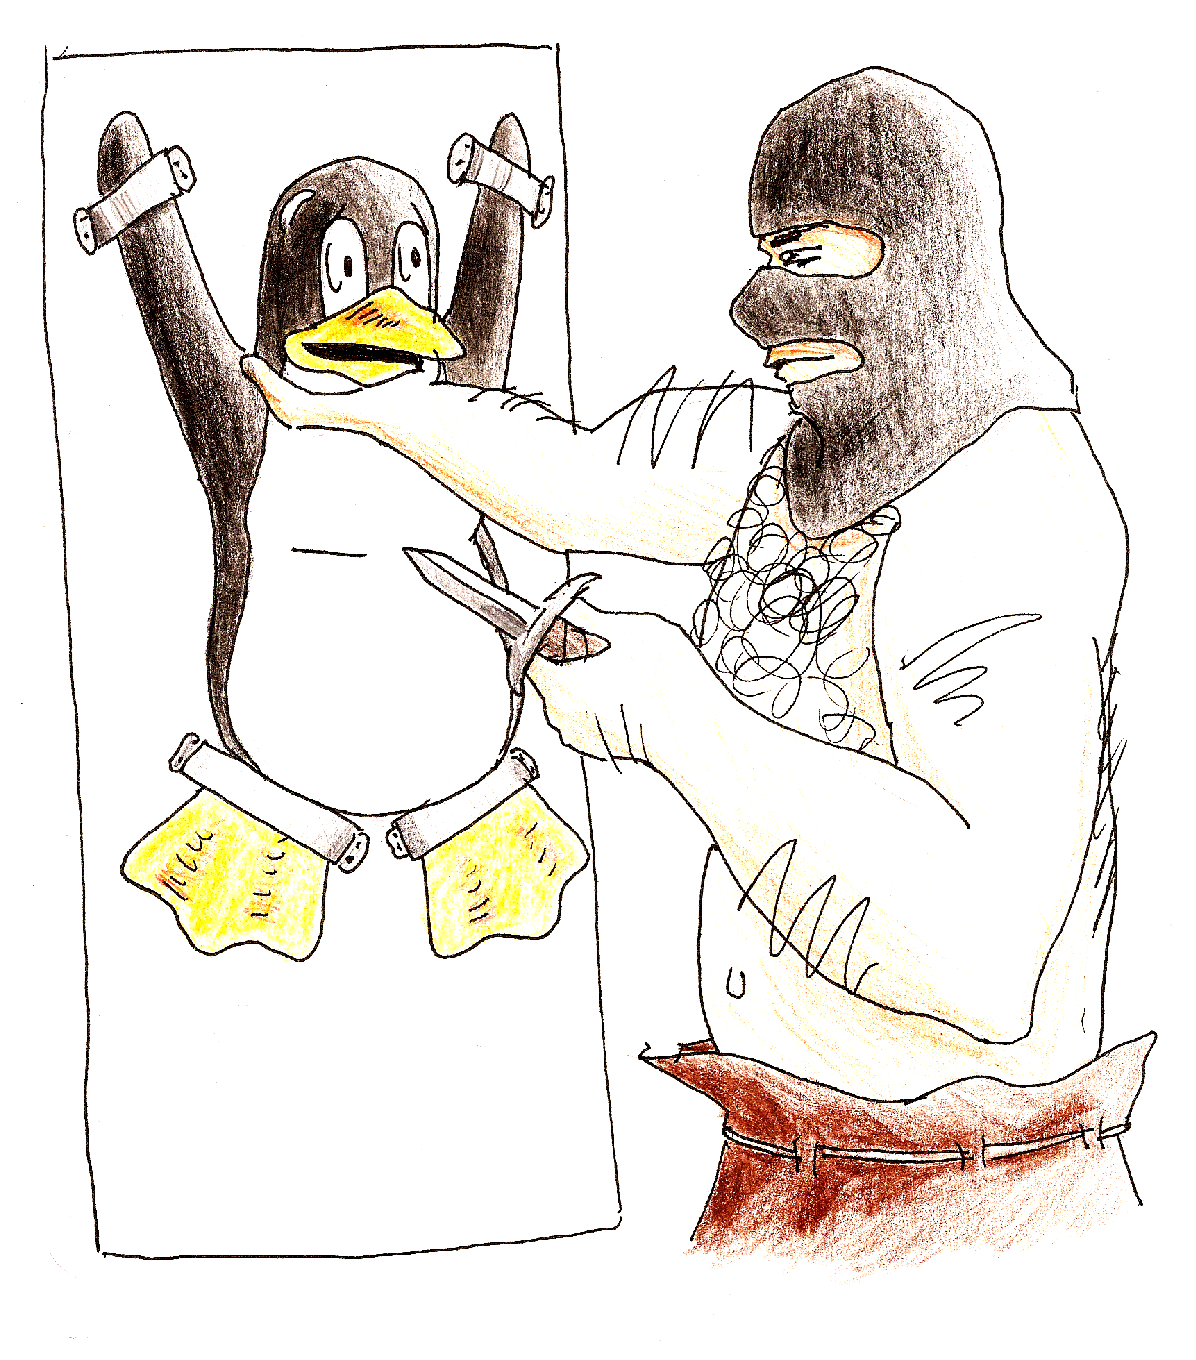
\includegraphics{cartoons/TortureTux}}
\caption{Validation and the Geneva Convention}
\ContributedBy{Figure}{fig:debugging:Validation and the Geneva Convention}{Melissa Broussard}
\end{figure}

\begin{figure}[tb]
\centering
\resizebox{2in}{!}{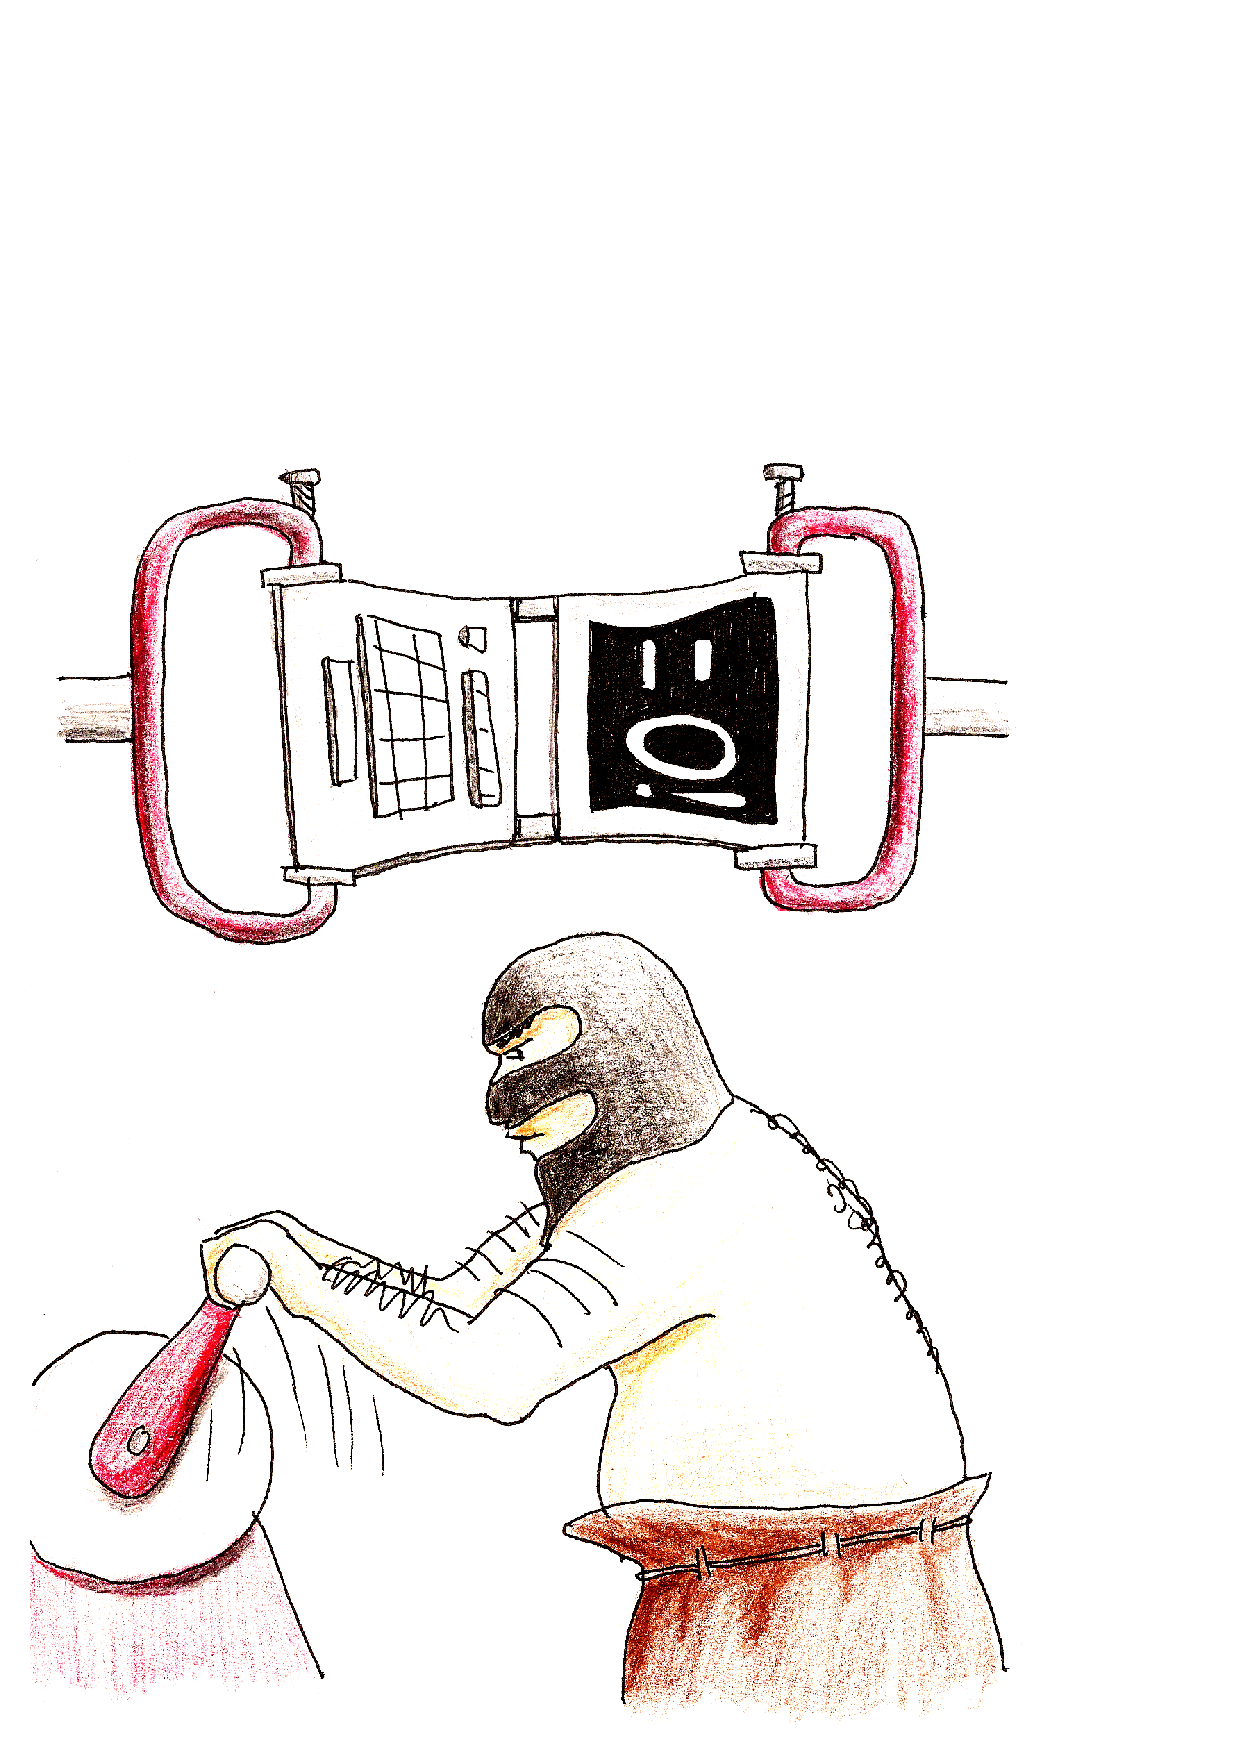
\includegraphics{cartoons/TortureLaptop}}
\caption{Rationalizing Validation}
\ContributedBy{Figure}{fig:debugging:Rationalizing Validation}{Melissa Broussard}
\end{figure}

어떤 사람들은 격렬한 검증을
Figure~\ref{fig:debugging:Validation and the Geneva Convention}
에 보인 것처럼 고문의 형태로 생각할 수도 있겠습니다.\footnote{
	우리 사이의 냉소는 이 사람들이 검증이 그들이 고쳐야 하게 될 버그를
	찾을지 두려워할지도 모르겠다는 질문을 낼지도 모르겠습니다.}
그런 사람들은 Tux 만화와는 별개로,
Figure~\ref{fig:debugging:Rationalizing Validation} 에 보인 것처럼 그들이
정말로 애니메이션화 될 수 없는 객체를 고문하고 있음을 상기하는게 좋을 수도
있습니다.
그렇지 않은 사람들은 자신의 코드를 고문하는데 실패하면 그 코드가 자신을 고문할
수 있음을 알아 두십시오!

그러나, 이는 프로젝트의 생애 중 구체적으로 언제 검증을 시작해야 하는지 질문을
던지는데, 다음 섹션에서 이 주제를 다룹니다.

\iffalse

Some people might see vigorous validation as a form of torture, as
depicted in
Figure~\ref{fig:debugging:Validation and the Geneva Convention}.\footnote{
	The cynics among us might question whether these people are
	afraid that validation will find bugs that they will then be
	required to fix.}
Such people might do well to remind themselves that, Tux cartoons aside,
they are really torturing an inanimate object, as shown in
Figure~\ref{fig:debugging:Rationalizing Validation}.
Rest assured that those who fail to torture their code are doomed to be
tortured by it!

However, this leaves open the question of exactly when during the project
lifetime validation should start, a topic taken up by the next section.

\fi

\subsection{When Should Validation Start?}
\label{sec:debugging:When Should Validation Start?}

검증은 정확히 그 프로젝트가 시작될 때 시작되어야 합니다.

이를 자세히 보기 위해, 버그를 추적하는 것은 작은 것보다 큰 프로그램에서 훨씬 더
어려움을 생각하세요.
따라서, 버그를 추적하는데 필요한 시간과 노력을 최소화 하기 위해, 여러분은
코드의 작은 단위를 테스트 해야 합니다.
여러분이 이 방법으로 모든 버그를 찾지는 못하겠지만, 상당한 부분을 찾을 것이며,
그게 버그를 찾고 그걸 고치기에 훨씬 쉬울 겁니다.
이 단계에서의 테스트는 또한 여러분에게 여러분의 전반적 설계에 있는 큰 결함을
알려줘서 설계로 인해 망가진 코드를 짜는데 낭비하는 시간을 줄이게 도와줄 겁니다.

하지만 여러분의 설계를 검증하기 전에 왜 코드를 기다립니까?\footnote{
	고전적인 ``일단 코드를 짜야만 한다, 그러면 생각할 동기를 갖는다'' 라는
	말에도 불구하구요.}
바라건대 Chapter~\ref{chp:Hardware and its Habits}
와~\ref{chp:Tools of the Trade} 를 읽는 것이 안타깝게 흔한 설계 결함을 막는데
필요한 정보를 여러분에게 주었을 겁니다만, 여러분의 설계를 어떤 동료와
이야기하거나 단순히 그걸 써보는 것만으로도 추가적인 결함을 없애는 걸 도와줄
겁니다.

\iffalse

Validation should start exactly when the project starts.

To see this, consider that tracking down a bug is much harder in a large
program than in a small one.
Therefore, to minimize the time and effort required to track down bugs,
you should test small units of code.
Although you won't find all the bugs this way, you will find a substantial
fraction, and it will be much easier to find and fix the ones you do find.
Testing at this level can also alert you to larger flaws in your overall
design, minimizing the time you waste writing code that is broken
by design.

But why wait until you have code before validating your design?\footnote{
	The old saying ``First we must code, then we have incentive to
	think'' notwithstanding.}
Hopefully reading Chapters~\ref{chp:Hardware and its Habits}
and~\ref{chp:Tools of the Trade} provided you with the information
required to avoid some regrettably common design flaws,
but discussing your design with a colleague or even simply writing it
down can help flush out additional flaws.

\fi

하지만, 여러분이 설계가 있을 때까지 검증을 대기하는 것은 너무 오래 기다리는
것인 경우가 너무 많습니다.
여러분의 자연적인 수준의 긍정성이 여러분으로 하여금 여러분이 요구사항을 완전히
이해하기도 전에 설계를 시작하게 하지는 않았을까요?
이 질문에 대한 대답은 거의 항상 ``그렇다'' 입니다.
결함 있는 요구사항을 막는 한가지 좋은 방법은 여러분의 사용자를 아는 겁니다.
그들을 정말 잘 대접하려면, 여러분은 그들과 함께 살아봐야 합니다.

\iffalse

However, it is all too often the case that waiting to start validation
until you have a design is waiting too long.
Mightn't your natural level of optimism caused you to start the design
before you fully understood the requirements?
The answer to this question will almost always be ``yes''.
One good way to avoid flawed requirements is to get to know your users.
To really serve them well, you will have to live among them.

\fi

\QuickQuiz{
	제가 코딩을 시작하기도 전부터 이 검증 일을 하라고 말하는 거예요???
	그건 시작도 안하기에 아주 좋은 방법처럼 들리는데요!!!

	\iffalse

	You are asking me to do all this validation BS before
	I even start coding???
	That sounds like a great way to never get started!!!

	\fi

}\QuickQuizAnswer{
	그게 여러분의 프로젝트라면, 예를 들어 취미라면, 하고 싶은대로 하세요.
	여러분이 낭비하는 시간은 여러분 스스로의 것일 것이고, 그걸 위해
	여러분이 답변을 해야 할 질문을 던지는 사람도 없습니다.
	그리고 시간이 완전히 낭비되지 않을 기회도 있습니다.
	예를 들어, 여러분이 첫번째 종류의 프로젝트를 한다면, 그 요구사항은 어떤
	면에서는 어쨌건 알려지지 않았을 겁니다.
	이 경우, 최선의 방법은 여러개의 대략적 해결책들을 빠르게 프로토타이핑
	하고 그것들을 시도해 본 후, 뭐가 가장 잘 동작하는지 보는 겁니다.

	다른 한편, 여러분이 존재하는 시스템들과 상당히 비슷한 시스템을 만들도록
	돈을 받고 있다면, 여러분은 여러분의 사용자, 고용자, 그리고 미래의
	자신에게 일찍 그리고 자주 검증할 일을 빚지는 겁니다.

	\iffalse

	If it is your project, for example, a hobby, do what you like.
	Any time you waste will be your own, and you have no one else
	to answer to for it.
	And there is a good chance that the time will not be completely
	wasted.
	For example, if you are embarking on a first-of-a-kind project,
	the requirements are in some sense unknowable anyway.
	In this case, the best approach might be to quickly prototype
	a number of rough solutions, try them out, and see what works
	best.

	On the other hand, if you are being paid to produce a system that
	is broadly similar to existing systems, you owe it to your users,
	your employer, and your future self to validate early and often.

	\fi

}\QuickQuizEnd

첫번째 종류 프로젝트는 종종 급속 프로토타이핑이나 애자일과 같은 다른 방법론을
사용합니다.
여기서 이른 프로토타이핑의 주요 목표는 올바른 구현을 만드는게 아니라 그
프로젝트의 요구사항을 배우는 겁니다.
하지만 이는 여러분이 검증을 하지 않음을 의미하지 않습니다; 그건 여러분이 그걸
다르게 접근함을 의미합니다.

그런 방법 중 하나는 다윈주의 관점을 취하는데, 검증 도구가 그 문제를 해결하는데
맞지 않는 코드를 제거하게 합니다.
이 관점에서, 적극적 검증 도구는 여러분의 소프트웨어의 상요가능성을 위해
필수적입니다.
그러나, 이 방법을 그 논리적 결론을 위해 취하는 것은 상당히 겸손한 것인데, 이는
우리 개발자들이 우리의 주의깊게 만든 변경이 다윈주의 관점에서는 무작위적
기형이라는 것을 인정해야 하게 하기 때문입니다.
다른 한편으로, 이 결론은 수정의 7퍼센트는 최소 하나의 버그를 만든다는 오랜
경험으로~\cite{RexBlack2012SQA} 지지됩니다.

여러분의 검증 도구는 얼마나 적극적이어야 할까요?
그것이 찾는 버그가 여러분의 소프트웨어 설계의 토대를 위협하는게 아니라면, 그건
아직 충분히 적극적이지 않습니다.
어쨌건, 여러분의 설계는 여러분의 코드가 그런만큼 버그에 취약하며, 여러분이
여러분의 설계 내의 버그를 빨리 찾아서 고칠수록 그 설계 버그를 코딩하는데
낭비하는 시간을 줄일 수 있습니다.

\iffalse

First-of-a-kind projects often use different methodologies such as
rapid prototyping or agile.
Here, the main goal of early prototypes are not to create correct
implementations, but rather to learn the project's requirements.
But this does not mean that you omit validation; it instead means that
you approach it differently.

One such approach takes a Darwinian view, with the validation suite
eliminating code that is not fit to solve the problem at hand.
From this viewpoint, a vigorous validation suite is essential to the
fitness of your software.
However, taking this approach to its logical conclusion is quite humbling,
as it requires us developers to admit that our carefully crafted changes
to the codebase are, from a Darwinian standpoint, random mutations.
On the other hand, this conclusion is supported by long experience
indicating that seven percent of fixes introduce at least one
bug~\cite{RexBlack2012SQA}.

How vigorous should your validation suite be?
If the bugs it finds aren't threatening the very foundations of your
software design, then it is not yet vigorous enough.
After all, your design is just as prone to bugs as is your code, and
the earlier you find and fix the bugs in your design, the less time
you will waste coding those design bugs.

\fi

\QuickQuiz{
	소프트웨어의 정확성을 정말로 테스트 할 수 있다고 말하는 거예요???
	그게 불가능하다는 건 모두가 안다구요!!!

	\iffalse

	Are you actually suggesting that it is possible to test
	correctness into software???
	Everyone knows that is impossible!!!

	\fi

}\QuickQuizAnswer{
	이 글은 ``테스트'' 보다는 ``검증'' 이라는 단어를 사용함에 주의해
	주세요.
	``검증'' 은 테스팅에 더해 formal 한 방법을 포함하는데, 이에 대해 더
	자세한 내용을 위해선
	Chapter~\ref{chp:Formal Verification} 를 읽어 주세요.

	하지만 모두가 알아야 할 내용을 이야기 하는 동안은, 다윈의 진화는
	정확도에 대한 것이 아니라 생존에 대한 것임을 기억합시다.
	소프트웨어에서도 마찬가지입니다.
	개발자로서 저의 목표는 제 소프트웨어가 이론적 관점에서 매력적이게
	하는게 아니라 사용자가 무엇을 던져대든 생존하는 것입니다.

	정확성이라는 방향도 올바른 사용처가 있지만, 그것의 기본적 한계는 그
	정확도가 판정되는 기술서 역시 버그를 가진다는 것입니다.
	이는 해당 코드가 의도된 버그들을 가지고 있는지 증명하는 전통적 정확성
	증명 이상도 이하도 아님을 의미합니다!

	\iffalse

	Please note that the text used the word ``validation'' rather
	than the word ``testing''.
	The word ``validation'' includes formal methods as well as
	testing, for more on which please see
	Chapter~\ref{chp:Formal Verification}.

	But as long as we are bringing up things that everyone should
	know, let's remind ourselves that Darwinian evolution is
	not about correctness, but rather about survival.
	As is software.
	My goal as a developer is not that my software be attractive
	from a theoretical viewpoint, but rather that it survive
	whatever its users throw at it.

	Although the notion of correctness does have its uses, its
	fundamental limitation is that the specification against which
	correctness is judged will also have bugs.
	This means nothing more nor less than that traditional correctness
	proofs prove that the code in question contains the intended
	set of bugs!

	\fi

	정확성의 대안적 정의는 그 대신 문제가 되는 특성의 부재에 집중하는데,
	예를 들어 소프트웨어가 use-after-free 버그, \co{NULL} 포인터 역참조,
	array-out-of-bounds 참조 등이 없음을 증명하는 것입니다.
	실수하지 않고 그런 종류의 버그를 찾아서 제거하는건 매우 유용합니다.
	그러나 그런 종류의 버그의 부재는 어떤 특정 목표에 적합한지를 보이는
	데에는 어떤 일도 하지 않는다는 사실은 여전합니다.

	따라서, 사용처 기반 검증이 여전히 중요하게 남아있습니다.

	별개로, 여러부느이 소프트웨어의 정확성을 검증하는 것 역시 중요한데,
	특히 검증기와 명세서의 검증의 필요성을 놓고 보면 더욱 그렇습니다.

	\iffalse

	Alternative definitions of correctness instead focus on the
	lack of problematic properties, for example, proving that the
	software has no use-after-free bugs, no \co{NULL} pointer
	dereferences, no array-out-of-bounds references, and so on.
	Make no mistake, finding and eliminating such classes of bugs
	can be highly useful.
	But the fact remains that the lack of certain classes of bugs
	does nothing to demonstrate fitness for any specific purpose.

	Therefore, usage-driven validation remains critically important.

	Besides, it is also impossible to verify correctness into your
	software, especially given the problematic need to verify both
	the verifier and the specification.

	\fi

}\QuickQuizEnd

이 조언은 첫번째 종류의 프로젝트에 적용됨을 다시 반복할 가치가 있겠습니다.
만약 여러분이 그대신 잘 알려진 영역의 프로젝트를 한다면 이전의 경험으로부터
배우기를 거부하는 건 상당히 바보스러운 일이 될 겁니다.
하지만 여러분은 여전히 그 프로젝트의 시작 단계부터 검증을 시작해야 합니다만,
다른 사람들의 힘들게 얻어진 요구사항과 함정들에 안내를 받기 바랍니다.

똑같이 중요한 질문은 ``언제 검증이 멈춰야 하는가?'' 입니다.
최고의 답은 ``마지막 변경으로부터 얼마간 시간이 지난후'' 입니다.
모든 변경은 버그를 만들 잠재적 가능성이 있으며, 따라서 모든 변경이 검증되어야
합니다.
더 나아가, 검증 개발은 프로젝트의 생애 전체에 걸쳐 지속되어야 합니다.
어쨌건, 앞의 다윈주의 특성은 버그가 여러분의 검증 도구에 적응할 것을
암시합니다.
따라서, 여러분이 자신의 검증 도구를 계속해서 개선하지 않으면, 여러분의
프로젝트는 자연적으로 검증 도구에 면역이 있는 버그 무리를 쌓을 겁니다.

\iffalse

It is worth reiterating that this advice applies to first-of-a-kind
projects.
If you are instead doing a project in a well-explored area, you would
be quite foolish to refuse to learn from previous experience.
But you should still start validating right at the beginning of the
project, but hopefully guided by others' hard-won knowledge of both
requirements and pitfalls.

An equally important question is ``When should validation stop?''
The best answer is ``Some time after the last change.''
Every change has the potential to create a bug, and thus every
change must be validated.
Furthermore, validation development should continue through the
full lifetime of the project.
After all, the Darwinian perspective above implies that bugs are
adapting to your validation suite.
Therefore, unless you continually improve your validation suite, your
project will naturally accumulate hordes of validation-suite-immune bugs.

\fi

하지만 삶은 트레이드오프이고, 검증 도구에 투자되는 모든 시간은 프로젝트 자체를
개선하는데에는 직접적으로 투자될 수 없습니다.
이런 종류의 선택은 결코 쉽지 않으며, 검증에 지나치게 투자하는 것은 부족하게
투자하는 것만큼이나 문제가 됩니다.
하지만 이는 삶이 쉽지 않음을 알리는 또하나의 것일 뿐입니다.

이제 우리는 프로젝트의 시작 시점에 (더 빨리 할 수 없다면!) 검증을 시작해야 하며
검증과 검증 개발 모두 프로젝트의 생애 동안 지속되어야 함에 동의했으니 다음
섹션들은 그 가치가 증명된 여러 검증 기법들과 방법들을 다룹니다.

\iffalse

But life is a tradeoff, and every bit of time invested in validation
suites as a bit of time that cannot be invested in directly improving
the project itself.
These sorts of choices are never easy, and it can be just as damaging
to overinvest in validation as it can be to underinvest.
But this is just one more indication that life is not easy.

Now that we have established that you should start validation when
you start the project (if not earlier!), and that both validation and
validation development should continue throughout the lifetime of that
project, the following sections cover a number of validation techniques
and methods that have proven their worth.

\fi

\subsection{The Open Source Way}
\label{sec:debugging:The Open Source Way}

오픈소스 프로그래밍 방법론은 상당히 효과적이고 상당한 코드 리뷰와 테스트를
포함하는 것으로 증명되었습니다.

저는 개인적으로 오픈소스 커뮤니티의 상당한 코드 리뷰의 효과에 대해 증언할 수
있습니다.
리눅스 커널을 위한 제 첫번째 패치들은 한 노드의 메모리에 매핑해 둔 파일에 다른
노드가 쓰기를 할 수 있는 분산 파일시스템에 관련되어 있었습니다.
이 경우, 쓰기 오퍼레이션 동안 파일시스템의 일관성을 유지하기 위해 영향 받는
페이지를 그것의 메모리 매핑으로부터 무효화 시킬 필요가 있습니다.
저는 한 패치에서 첫번째 시도를 했으며, 오픈소스 격언인 ``빨리 보내고 자주
보내라'' 에 따라, 그 패치를 보냈습니다.
그리고 나서 저는 제가 그걸 어떻게 테스트 할지 생각했습니다.

\iffalse

The open-source programming methodology has proven quite effective, and
includes a regimen of intense code review and testing.

I can personally attest to the effectiveness of the open-source community's
intense code review.
One of my first patches to the Linux kernel involved a distributed
filesystem where one node might write to a given file that another node
has mapped into memory.
In this case, it is necessary to invalidate the affected pages from
the mapping in order to allow the filesystem to maintain coherence
during the write operation.
I coded up a first attempt at a patch, and, in keeping with the open-source
maxim ``post early, post often'', I posted the patch.
I then considered how I was going to test it.

\fi

하지만 저는 심지어 제가 전반적인 테스트 전략을 결정하기도 전에 제 패치에 대한
일부 버그를 지적하는 답장을 받았습니다.
저는 그 버그를 고치고 패치를 다시 보낸 후 저의 테스트 전략을 생각하기로
돌아왔습니다.
하지만, 제가 어떤 테스트 코드를 작성할 기회를 갖기 전에 저는 대시 보낸 패치에
대해 더 많은 버그를 지적하는 답장을 받았습니다.
이 과정은 그 자체로 여러번 반복되었으며, 저는 제가 이 패치를 정말로 테스트할
기회가 있긴 할지 확신할 수 없었습니다.

이 경험은 유명한 오픈소스 격언을 상기시켰습니다:
충분한 눈알이 있다면 모든 버그는 간단해진다~\cite{EricSRaymond99b}.

그러나, 여러분이 어떤 코드나 패치를 보내기 전에 약간의 질문을 던쳐볼 가치가
있습니다:

\iffalse

But before I could even decide on an overall test strategy, I got a
reply to my posting pointing out a few bugs.
I fixed the bugs and reposted the patch, and returned to thinking
out my test strategy.
However, before I had a chance to write any test code, I received
a reply to my reposted patch, pointing out more bugs.
This process repeated itself many times, and I am not sure that I
ever got a chance to actually test the patch.

This experience brought home the truth of the open-source saying:
Given enough eyeballs, all bugs are shallow~\cite{EricSRaymond99b}.

However, when you post some code or a given patch, it is worth
asking a few questions:

\fi

\begin{enumerate}
\item	그 수많은 눈알 중 얼마나 많은 눈알이 정말로 여러분의 코드를 볼까요?
\item	그 중 얼만큼이 여러분의 버그를 정말 찾기 충분할 정도로 경험 많고
	현명할까요?
\item	그것들은 구체적으로 언제 코드를 보기 시작할까요?

\iffalse

\item	How many of those eyeballs are actually going to look at your code?
\item	How many will be experienced and clever enough to actually find
	your bugs?
\item	Exactly when are they going to look?

\fi

\end{enumerate}

저는 운이 좋았습니다:  제 패치로 제공된 기능을 원한 사람이 누군가 있었는데, 그
사람은 분산 파일시스템에 오랜 경험이 있었고, 거의 곧바로 제 패치를 들여다
보았습니다.
아무도 제 패치를 들여다보지 않았다면, 리뷰도 없었을 것이고 따라서 그 버그들 중
어떤 것도 발견되지 않았을 겁니다.
제 패치를 들여다 본 살마들이 분산 파일시스템에 대한 경험이 없었다면, 그들이 그
모드 버그를 찾았을 가능성은 낮습니다.
그들이 몇달 또는 심지어 몇년간 코드를 보기를 미뤘다면, 전 그 패치가 어떻게
동작할 것으로 여겨졌는지 잊어서 그걸 고치기를 훨씬 어렵게 했을 가능성이
높습니다.

그러나, 우린 오픈소스 개발의 두번째 주의인 상당한 테스트를 잊지 말아야 합니다.
예를 들어, 엄청나게 많은 사람들이 리눅스 커널을 테스트 합니다.
어떤 사람들은 패치들을 제출되자마자, 아마 여러분의 것을 포함해, 테스트합니다.
또다른 사람들은 -next 트리를 테스트 하는데, 이는 도움이 되지만 여러분이 그
패치를 작성한 시점으로부터 그것들이 -next 트리에 들어가기까지는 몇주에서
몇달까지도 지연이 있을 수 있기 때문에 그 패치는 여러분의 마음 속에서 그렇게
싱싱하지는 않을 겁니다.
또다른 어떤 사람들은 메인테이너의 트리들을 테스트 하는데, 종종 비슷한 시간
지연이 있곤 합니다.

\iffalse

I was lucky:  There was someone out there who wanted the functionality
provided by my patch, who had long experience with distributed filesystems,
and who looked at my patch almost immediately.
If no one had looked at my patch, there would have been no review, and
therefore none of those bugs would have been located.
If the people looking at my patch had lacked experience with distributed
filesystems, it is unlikely that they would have found all the bugs.
Had they waited months or even years to look, I likely would have forgotten
how the patch was supposed to work, making it much more difficult to
fix them.

However, we must not forget the second tenet of the open-source development,
namely intensive testing.
For example, a great many people test the Linux kernel.
Some test patches as they are submitted, perhaps even yours.
Others test the -next tree, which is helpful, but there is likely to be
several weeks or even months delay between the time that you write the
patch and the time that it appears in the -next tree, by which time the
patch will not be quite as fresh in your mind.
Still others test maintainer trees, which often have a similar time delay.

\fi

약간의 사람들은 코드가 메인라인 또는 마스터 소스 트리에 (리눅스 커널의 경우
Linus 의 트리) 들어가기 전까지 테스트 하지 않습니다.
여러분의 메인테이너가 여러분의 패치를 테스트 되기 전까지 받아들이지 않는다면,
이는 여러분에게 데드락 상황을 일으킵니다: 여러분의 패치는 테스트 되기 전까지
받아들여지지 않는데 그것은 받아들여지기 전까지 테스트 되지 않을 겁니다.
그러나, 많은 사람들과 단체가 코드가 리눅스 배포판에 들어가기 전까지는 테스트
하지 않음을 놓고 보면 메인라인 코드를 테스트 하는 사람들은 여전히 상대적으로
적극적입니다.

그리고 어떤 사람이 여러분의 패치를 테스트 한다고 해도, 그들이 여러분의 버그를
찾는데 필요한 하드웨어와 소프트웨어 구성과 워크로드를 수행할지는 보장되지
않습니다.

\iffalse

Quite a few people don't test code until it is committed to mainline,
or the master source tree (Linus's tree in the case of the Linux kernel).
If your maintainer won't accept your patch until it has been tested,
this presents you with a deadlock situation: your patch won't be accepted
until it is tested, but it won't be tested until it is accepted.
Nevertheless, people who test mainline code are still relatively
aggressive, given that many people and organizations do not test code
until it has been pulled into a Linux distro.

And even if someone does test your patch, there is no guarantee that they
will be running the hardware and software configuration and workload
required to locate your bugs.

\fi

따라서, 오픈소스 프로젝트를 위한 코드를 작성할 때라 해도 여러분은 여러분 자신의
테스트 도구를 개발하고 수행할 준비를 해야 합니다.
테스트 개발은 제대로 가치를 평가받지 못했지만 가치있는 기술이므로 사용 가능한
존재하는 테스트 도구들의 모든 이점을 취하십시오.
테스트 개발의 중요성 탓에 우린 그에 대한 더 많은 이야기를 그 주제 전용의 책에
남겨야 하겠습니다.
따라서 다음 섹션들은 여러분이 이미 좋은 테스트 도구를 가지고 있다는 가정 하에
여러분의 코드의 버그를 찾는 방법에 대해 이야기 합니다.

\iffalse

Therefore, even when writing code for an open-source project, you need to
be prepared to develop and run your own test suite.
Test development is an underappreciated and very valuable skill, so be
sure to take full advantage of any existing test suites available to
you.
Important as test development is, we must leave further discussion of it
to books dedicated to that topic.
The following sections therefore discuss locating bugs in your code given that
you already have a good test suite.

\fi

\section{Tracing}
\label{sec:debugging:Tracing}
%
\epigraph{The machine knows what is wrong.  Make it tell you.}{\emph{Unknown}}

모든게 실패하면, \co{printk()} 를 추가하세요!
또는, 여러분이 사용자 모드 C 언어 어플리케이션을 작업하고 있다면, \co{printf()}
를요.

이유는 간단합니다: 어떻게 수행이 코드의 특정 포인트에 이르렀는지 모르겠다면,
뭐가 일어났는지 알기 위해 그 코드의 앞부분에 print 문을 뿌려두세요.
(사용자 어플리케이션을 위해) gdb 또는 (리눅스 커널 디버깅을 위해) kgdb 를
사용해서 비슷한 효과를 더 편리하고 유연하게 얻을 수 있습니다.
훨씬 더 정교한 도구들이 존재하는데, 최근의 것들은 실패 지점으로부터 시간을
되돌리는 기능도 제공합니다.

이런 간단한 테스트 도구들은 모두 가치있는데, 대부분의 시스템이 64K 이상의
메모리와 4\,MHz 보다 빠른 CPU 를 갖는 지금은 더욱 그렇습니다.
이런 도구들을 위한 많은 서적이 있으므로, 이 챕터는 약간만 더 이야기 하겠습니다.

\iffalse

When all else fails, add a \co{printk()}!
Or a \co{printf()}, if you are working with user-mode C-language applications.

The rationale is simple: If you cannot figure out how execution reached
a given point in the code, sprinkle print statements earlier in the
code to work out what happened.
You can get a similar effect, and with more convenience and flexibility,
by using a debugger such as gdb (for user applications) or kgdb
(for debugging Linux kernels).
Much more sophisticated tools exist, with some of the more recent
offering the ability to rewind backwards in time from the point
of failure.

These brute-force testing tools are all valuable, especially now
that typical systems have more than 64K of memory and CPUs running
faster than 4\,MHz.
Much has been
written about these tools, so this chapter will add only a little more.

\fi

그러나, 이런 도구들은 모두 여러분의 fastpath 에서 뭐가 잘못되고 있는지 보려고
할 때 심각한 단점을 보이는데, 이 도구들은 종종 지나친 오버헤드를 갖는다는
것입니다.
이런 목적을 위한 특수한 추적 도구가 있는데, 실행 시간 데이터 수집의 오버헤드를
최소화 하기 위해 데이터 소유권 기법을
(Chapter~\ref{chp:Data Ownership} 를 보세요)
사용합니다.
리눅스 커널에서의 한가지 예는 ``trace
events''~\cite{StevenRostedt2010perfTraceEventP1,StevenRostedt2010perfTraceEventP2,StevenRostedt2010perfTraceEventP3,StevenRostedt2010perfHP+DeathlyMacros}
로, 극단적으로 낮은 오버헤드를 가지고 데이터를 수집할 수 있게 하는 CPU 별
버퍼를 사용합니다.
심지어 그렇다고 해도 추적 기능을 켜는 것은 때로는 버그를 숨기기 충분할 정도로
타이밍을 바꿀 수 있어서
Section~\ref{sec:debugging:Probability and Heisenbugs} 과
특히 Section~\ref{sec:debugging:Hunting Heisenbugs} 에서 이야기한
\emph{heisenbug} 를 초래할 수 있습니다.
커널에서, BPF 는 커널 내의 데이터를 줄일 수 있어서, 커널에서 userspace 로의
정보 교환 오버헤드를 줄일 수 있습니다~\cite{BrendanGregg2019BPFperftools}.
Userspace 코드에서는 여러분을 도울 수 있는 도구가 굉장히 많습니다.
Brendan Gregg 의 블로그가 시작하기에 좋을 겁니다.\footnote{
	\url{http://www.brendangregg.com/blog/}}

\iffalse

However, these tools all have a serious shortcoming when you need a
fastpath to tell you what is going wrong, namely, these tools often have
excessive overheads.
There are special tracing technologies for this purpose, which typically
leverage data ownership techniques
(see Chapter~\ref{chp:Data Ownership})
to minimize the overhead of runtime data collection.
One example within the Linux kernel is
``trace events''~\cite{StevenRostedt2010perfTraceEventP1,StevenRostedt2010perfTraceEventP2,StevenRostedt2010perfTraceEventP3,StevenRostedt2010perfHP+DeathlyMacros},
which uses per-CPU buffers to allow data to be collected with
extremely low overhead.
Even so, enabling tracing can sometimes change timing enough to
hide bugs, resulting in \emph{heisenbugs}, which are discussed in
Section~\ref{sec:debugging:Probability and Heisenbugs}
and especially Section~\ref{sec:debugging:Hunting Heisenbugs}.
In the kernel, BPF can do data reduction in the kernel, reducing
the overhead of transmitting the needed information from the kernel
to userspace~\cite{BrendanGregg2019BPFperftools}.
In userspace code, there is a huge number of tools that can help you.
One good starting point is Brendan Gregg's blog.\footnote{
	\url{http://www.brendangregg.com/blog/}}

\fi

여러분이 heisenbug 를 막는다 하더라도, 다른 문제들이 여러분을 기다립니다.
예를 들어, 기계는 정말 모든 걸 알고 있다 하더라도, 그것이 아는 것은 거의 항상
여러분의 머리가 다룰 수 있는것보다 많습니다.
이런 이유로, 높은 품질의 테스트 도구들은 일반적으로 큰 결과를 분석하는 고도화된
스크립트를 갖춥니다.
하지만 알아두세요---스크립트는 여러분이 그것에게 말해달라는 것만 말합니다.
제 rcutorture 스크립트는 그런 점에서 한 예입니다: 그 스크립트의 초기 버전은 RCU
grace period 가 무한정 멈춰있는 테스트에 대해 만족을 했습니다.
이는 물론 RCU grace period 멈춤을 탐지하기 위한 수정을 초래했지만, 그
스크립트가 제가 그것들에게 찾으라고 한 문제들만을 찾을 것이라는 사실은 변하지
않습니다.
하지만 여러분이 탄탄한 설계를 갖지 않는다면 여러분은 여러분의 스크립트가 무엇을
검사해야 하는지 모를 수 있음을 명심하세요!

특히 \co{printk()} 호출과 관련한 추적의 또다른 문제는 그 오버헤드가
제품단계에서의 사용을 금지시킬 수 있다는 것입니다.
그런 경우엔 단정문이 도움이 됩니다.

\iffalse

Even if you avoid heisenbugs, other pitfalls await you.
For example, although the machine really does know all,
what it knows is almost always way more than your head can hold.
For this reason, high-quality test suites normally come with sophisticated
scripts to analyze the voluminous output.
But beware---scripts will only notice what you tell them to.
My \co{rcutorture} scripts are a case in point: Early versions of those
scripts were quite satisfied with a test run in which RCU grace periods
stalled indefinitely.
This of course resulted in the scripts being modified to detect RCU
grace-period stalls, but this does not change the fact that the scripts
will only detect problems that I make them detect.
But note well that unless you have a solid design, you won't know what
your script should check for!

Another problem with tracing and especially with \co{printk()} calls
is that their overhead can rule out production use.
In such cases, assertions can be helpful.

\fi

\section{Assertions}
\label{sec:debugging:Assertions}
%
\epigraph{No man really becomes a fool until he stops asking questions.}
	 {\emph{Charles P. Steinmetz}}

Assertions are usually implemented in the following manner:

\begin{VerbatimN}
if (something_bad_is_happening())
	complain();
\end{VerbatimN}

이 패턴은 종종 C 전처리기 매크로나 언어 내재 기능 안에 들어가게 되는데 예를
들면 리눅스 커널에서는 \co{WARN_ON(something_bad_is_happening())} 으로
표현됩니다.
물론, \co{something_bad_is_happening()} 이 종종 사실이라면, 결과 출력물은 다른
문제들을 숨길수도 있는 보고서가 될 것이므로,
\co{WARN_ON_ONCE(something_bad_is_happening())} 가 더 적절할 겁니다.

\iffalse

This pattern is often encapsulated into C-preprocessor macros or
language intrinsics, for example, in the Linux kernel, this might
be represented as \co{WARN_ON(something_bad_is_happening())}.
Of course, if \co{something_bad_is_happening()} quite frequently,
the resulting output might obscure reports of other problems,
in which case
\co{WARN_ON_ONCE(something_bad_is_happening())} might be more appropriate.

\fi

\QuickQuiz{
	\co{WARN_ON_ONCE()} 를 어떻게 구현할 수 있나요?

	\iffalse

	How can you implement \co{WARN_ON_ONCE()}?

	\fi

}\QuickQuizAnswer{
	여러분이 \co{WARN_ON_ONCE()} 가 가끔은 두번 이상 경고를 하는게
	괜찮다면, 간단하게 0 으로 초기화 되는 static 변수를 두세요.
	그 조건이 일어났을 때, 그 변수를 검사하고 그게 0 이 아니면 리턴하세요.
	그렇지 않다면, 그것을 1 로 바꾸고 메세지를 출력하고 리턴하세요.

	그 메세지가 정말로 한번 넘게 발생하지 않아야 한다면 위의 ``1 로
	바꾸고'' 대신 어토믹 교환 오퍼레이션을 사용할 수 있습니다.
	그 어토믹 교환 오퍼레이션이 0을 리턴할 때에만 메세지를 출력하세요.

	\iffalse

	If you don't mind \co{WARN_ON_ONCE()} sometimes warning more
	than once, simply maintain a static variable that is initialized
	to zero.
	If the condition triggers, check the variable, and
	if it is non-zero, return.
	Otherwise, set it to one, print the message, and return.

	If you really need the message to never appear more than once,
	you can use an atomic exchange operation in place of ``set it
	to one'' above.
	Print the message only if the atomic exchange operation returns
	zero.

	\fi

}\QuickQuizEnd

병렬 코드에서 일어날 수도 있는 한가지 나쁜 무언가는 특정 락을 잡은 상태에서
호출될 것으로 예상되는 함수가 그 락을 잡지 않은채 호출되는 것입니다.
그런 함수는 가끔 ``호출자는 \co{foo_lock} 을 잡고서만 이 함수를 호출해야 함''
같은 무언가를 그 함수의 머리부분 주석에 가지고 있습니다만, 그런 주석은 누군가가
그걸 정말로 읽지 않는다면 좋은 일을 하지 않습니다.
수행가능한 문장이 훨씬 많은 가치를 제공합니다.
그래서 리눅스 커널의 lockdep
기능은~\cite{JonathanCorbet2006lockdep,StevenRostedt2011locdepCryptic}  특정
락이 잡혀져 있는지 검사하는 \co{lockdep_assert_held()} 함수를 제공합니다.
물론, lockdep 은 상당한 오버헤드를 일으키며, 따라서 제품에서는 도움이 되지 않을
수도 있습니다.

\iffalse

In parallel code, one bad something that might happen is that
a function expecting to be called under a particular lock might be called
without that lock being held.
Such functions sometimes have header comments stating something like
``The caller must hold \co{foo_lock} when calling this function'', but
such a comment does no good unless someone actually reads it.
An executable statement carries far more weight.
The Linux kernel's lockdep
facility~\cite{JonathanCorbet2006lockdep,StevenRostedt2011locdepCryptic}
therefore provides a \co{lockdep_assert_held()} function that checks
whether the specified lock is held.
Of course, lockdep incurs significant overhead, and thus might not be
helpful in production.

\fi

병렬 코드에서의 특히나 나쁜 무언가는 데이터로의 예상되지 못한 동시의
접근입니다.
Kernel Concurrency Sanitizer (KCSAN)~\cite{JonathanCorbet2019KCSAN} 은
\co{READ_ONCE()} 와 \co{WRITE_ONCE()} 같은 존재하는 표시를 어떤 액세스가 경고
메세지를 낼 가치가 있는지 아는데 사용합니다.
KCSAN 은 상당한 false-positive 비율을 갖는데, C 를 어셈블리어에 추가적 문법을
가진 것으로 생각하는 개발자의 관점에서는 특히나 그렇습니다.
따라서 KCSAN 은 알려진 데이터 경쟁을 포기하기 위해 \co{data_race()} 기능을
제공하며, 데이터 경쟁을 명시적으로 검사하기 위해 \co{ASSERT_EXCLUSIVE_ACCESS()}
와 \co{ASSERT_EXCLUSIVE_WRITER()} 또한
제공합니다~\cite{MarcoElver2020FearDataRaceDetector1,MarcoElver2020FearDataRaceDetector2}.

그러니 검사가 필요한 곳에서 뭘 할 수 있느냐는 알겠는데, 실행시간 검사
오버헤드가 허용될 수 없는 경우에는 어떡하죠?
한가지 방법은 정적 분석으로, 다음 섹션에서 다룹니다.

\iffalse

An especially bad parallel-code something is unexpected concurrent
access to data.
The Kernel Concurrency Sanitizer (KCSAN)~\cite{JonathanCorbet2019KCSAN}
uses existing markings such as \co{READ_ONCE()} and \co{WRITE_ONCE()}
to determine which concurrent accesses deserve warning messages.
KCSAN has a significant false-positive rate, especially from the
viewpoint of developers thinking in terms of C as assembly language
with additional syntax.
KCSAN therefore provides a \co{data_race()} construct to forgive
known-benign data races, and also the \co{ASSERT_EXCLUSIVE_ACCESS()}
and \co{ASSERT_EXCLUSIVE_WRITER()} assertions to explicitly check
for data races~\cite{MarcoElver2020FearDataRaceDetector1,MarcoElver2020FearDataRaceDetector2}.

So what can be done in cases where checking is necessary, but where the
overhead of runtime checking cannot be tolerated?
One approach is static analysis, which is discussed in the next section.

\fi

\section{Static Analysis}
\label{sec:debugging:Static Analysis}
%
\epigraph{A lot of automation isn't a replacement of
	  humans but of mind-numbing behavior.}
	 {\emph{Summarized from Stewart Butterfield}}

정적 분석은 한 프로그램이 다른 프로그램을 입력으로 받고 해당 프로그램에 있는
에러와 취약점을 보고하는 하나의 검증 기법입니다.
흥미롭게도, 거의 모든 프로그램이 컴파일러나 인터프리터를 통해 정적 분석 됩니다.
이 도구들은 완벽과는 거리가 멀지만 에러를 찾아내는 기술은 지난 수십년간 상당히
개선되었는데, 부분적으로는 분석을 진행하는데 64K 바이트보다 훨씬 큰 메모리를
사용할 수 있게 되었기 때문입니다.

원래의 UNIX \co{lint} 도구는~\cite{StephenJohnson1977lint} 상당히 유용했는데,
그것의 기능들 중 상당히 많은 것들이 C 컴파일러에 들어오긴 했습니다.
그러나 오늘날 사용되고 있는 link 같은 도구들이 있습니다.
Sparse 정적 분석기는~\cite{JonathanCorbet2004sparse} 다음의 것들을 퐇마한
리눅스 커널의 고수준 문제들을 찾아냅니다.

\iffalse

Static analysis is a validation technique where one program takes a second
program as input, reporting errors and vulnerabilities located in this
second program.
Interestingly enough, almost all programs are statically analyzed
by their compilers or interpreters.
These tools are far from perfect, but their ability to locate
errors has improved immensely over the past few decades, in part because
they now have much more than 64K bytes of memory in which to carry out their
analyses.

The original UNIX \co{lint} tool~\cite{StephenJohnson1977lint} was
quite useful, though much of its functionality has since been incorporated
into C compilers.
There are nevertheless lint-like tools in use to this day.
The sparse static analyzer~\cite{JonathanCorbet2004sparse}
finds higher-level issues in the Linux kernel, including:

\fi

\begin{enumerate}
\item	User-space 구조체로의 포인터의 잘못된 사용.
\item	너무 긴 상수로부터의 값 할당.
\item	빈 \co{switch} 문.
\item	맞지 않는 락 획득과 해제 기능들.
\item	잘못된 per-CPU 기능의 사용.
\item	RCU 포인터가 아닌 것에의 RCU 기능 사용과 그 반대.

\iffalse

\item	Misuse of pointers to user-space structures.
\item	Assignments from too-long constants.
\item	Empty \co{switch} statements.
\item	Mismatched lock acquisition and release primitives.
\item	Misuse of per-CPU primitives.
\item	Use of RCU primitives on non-RCU pointers and vice versa.

\fi

\end{enumerate}

컴파일러가 자신의 정적 분석 기능을 계속해서 늘려갈 것으로 보이지만, 이 sparse
정적 분석기는 컴파일러 바깥에서의 정적 분석의 장점, 특히 어플리케이션 특수
버그의 탐색을 선보입니다.
\Crefrange{sec:formal:SAT Solvers}{sec:formal:Stateless Model Checkers}
는 더 정교한 형태의 정적 분석을 설명합니다.

\iffalse

Although it is likely that compilers will continue to increase their
static-analysis capabilities, the sparse static analyzer demonstrates
the benefits of static analysis outside of the compiler, particularly
for finding application-specific bugs.
\Crefrange{sec:formal:SAT Solvers}{sec:formal:Stateless Model Checkers}
describe more sophisticated forms of static analysis.

\fi

\section{Code Review}
\label{sec:debugging:Code Review}
%
\epigraph{If a man speaks of my virtues, he steals from me;
	  if he speaks of my vices, then he is my teacher.}
	 {\emph{Chinese proverb}}

코드 리뷰는 인간이 분석을 하는 정적 분석의 특수한 형태입니다.
이 섹션은 검사 (inspection), 수행 따라가기 (walkthroughs), 그리고 자가 검진
(self-inspection) 을 다룹니다.

\iffalse

Code review is a special case of static analysis with human beings doing
the analysis.
This section covers inspection, walkthroughs, and self-inspection.

\fi

\subsection{Inspection}
\label{sec:debugging:Inspection}

전통적으로 정식 코드 검사는 정식으로 정의된 역할을 가지고 대면 회의에서
수행됩니다: 운영자, 개발자, 그리고 한명 혹은 두명의 참여자들.
개발자는 코드를 읽어나가며 그게 무엇을 하고 왜 동작하는지 설명합니다.
한명 혹은 두명의 참여자들은 질문을 던지고 문제를 제기하여, 저자의 잘못된 가정을
드러내길 바라며, 운영자의 역할은 발생하는 충돌을 처리하고 기록을 하는 것입니다.
이 과정은 버그를 찾는데 굉장히 효과적인데, 특히 모든 참여자가 해당 코드에
친숙하면 그렇습니다.

그러나, 이 대면 정식 진행은 세계의 리눅스 커널 공동체에서는 잘 동작하지 않을 수
있습니다.
그대신, 각 개인들은 분리된 채로 코드를 리뷰하고 이메일이나 IRC 를 통해 의견을
제공합니다.
기록 남기기는 이메일 기록이나 IRC 로그를 통해 제공되며, 운영자는 간혹 발생하는
의견 대립 시에 자발적으로 서비스를 제공합니다.
이 프로세스는 합리적 수준으로 잘 동작하는데, 모든 참여자가 해당 코드에 친숙할
때 특히 그렇습니다.
실제로, 전통적인 정식 분석 대비 리눅스 커널 공동체 방식의 장점 중 하나는 코드에
친숙하지 \emph{않은}, 따라서 저자의 잘못된 가정에 의해 눈이 가려지지 않고
코드를 테스트 할수도 있는 사람들의 기여 확률이 높다는 것입니다.

\iffalse

Traditionally, formal code inspections take place in face-to-face meetings
with formally defined roles: moderator, developer, and one or two other
participants.
The developer reads through the code, explaining what it is doing and
why it works.
The one or two other participants ask questions and raise issues,
hopefully exposing the author's invalid assumptions, while the moderator's
job is to resolve any resulting conflicts and take notes.
This process can be extremely effective at locating bugs, particularly
if all of the participants are familiar with the code at hand.

However, this face-to-face formal procedure does not necessarily
work well in the global Linux kernel community.
Instead, individuals review code separately and provide comments via
email or IRC\@.
The note-taking is provided by email archives or IRC logs, and moderators
volunteer their services as required by the occasional flamewar.
This process also works reasonably well, particularly if all of the
participants are familiar with the code at hand.
In fact, one advantage of the Linux kernel community approach over
traditional formal inspections is the greater probability of contributions
from people \emph{not} familiar with the code, who might not be blinded
by the author's invalid assumptions, and who might also test the code.

\fi

\QuickQuiz{
	숨겨져 있는 리눅스 커널 해커들의 어떤 잘못된 가정을 당신은 이야기 하는
	건가요???

	\iffalse

	Just what invalid assumptions are you accusing Linux kernel
	hackers of harboring???

	\fi

}\QuickQuizAnswer{
	이 질문에 대한 완벽한 답을 원하는 사람들은 ``Fixes:'' 문자를 가지고
	있는 커밋들을 리눅스 커널 \co{git} 저장소에서 검색해 보세요.
	그런 것들이 2020년에는 수천개가 있는데, 아래의 잘못된 가정을 위한
	수정들을 포함합니다:

	\iffalse

	Those wishing a complete answer to this question are encouraged
	to search the Linux kernel \co{git} repository for commits
	containing the string \co{Fixes:}.
	There were many thousands of them just in the year 2020, including
	fixes for the following invalid assumptions:

	\fi

	\begin{enumerate}
	\item	0이 아닌 분모에 대한 검사가 divide-by-zero 에러를 막는다.
		(힌트: 테스트는 64비트 오퍼레이터를 사용하는데 나누기는 32비트
		오퍼레이터를 사용한다고 생각해 보세요.)
	\item	Userspace 는 커널과 통신하는데 사용되는 버전 관리된 데이터
		구조를 0으로 초기화 한다고 신뢰될 수 있다.
		(힌트: 가끔 userspace 는 그 데이터 구조가 얼마나 큰지 모를 때가
		있습니다.)
	\item	오래되어 유효하지않은 TCP duplicate selective acknowledgement
		(D-SACK) 패킷은 완전히 무시될 수 있다.
		(힌트: 이 패킷은 다른 정보도 담고 있을수도 있습니다.)
	\item	모든 CPU 는 little-endian 을 사용한다.
	\item	데이터 구조가 더이상 필요하지 않아지면 그 메모리는 즉시
		해제된다.
	\item	모든 기기는 대기 모드인 상태에서 초기화 될 수 있다.
	\item	개발자들은 올바른 16진수 산수를 일관적으로 할거라 신뢰될 수
		있다.

	\iffalse

	\item	Testing for a non-zero denominator will prevent
		divide-by-zero errors.
		(Hint: Suppose that the test uses 64-bit arithmetic
		but that the division uses 32-bit arithmetic.)
	\item	Userspace can be trusted to zero out versioned data
		structures used to communicate with the kernel.
		(Hint: Sometimes userspace has no idea how large the
		data structure is.)
	\item	Outdated TCP duplicate selective acknowledgement (D-SACK)
		packets can be completely ignored.
		(Hint: These packets might also contain other information.)
	\item	All CPUs are little-endian.
	\item	Once a data structure is no longer needed, all of its
		memory may be immediately freed.
	\item	All devices can be initialized while in standby mode.
	\item	Developers can be trusted to consistently do correct
		hexidecimal arithmetic.

	\fi

	\end{enumerate}

	이 커밋들을 더 자세히 들여다보는 분들은 잘못된 가정은 예외가 아니라
	규칙이라는 결론을 내릴 겁니다.

	\iffalse

	Those who look at these commits in greater detail will conclude
	that invalid assumptions are the rule, not the exception.

	\fi

}\QuickQuizEnd

리눅스 커널 공동체의 리뷰 프로세스는 개선의 여지가 분명 있을 것입니다:

\iffalse

It is quite likely that the Linux kernel community's review process
is ripe for improvement:

\fi

\begin{enumerate}
\item	가끔은 효과적인 리뷰를 하기에 필요한 시간과 전문성을 가진 사람이
	부족합니다.
\item	모든 리뷰 토론이 기록된다고는 하지만, 통찰이 잊혀지고 사람들이 토론을
	찾아내는데 실패함으로써 ``소실'' 되고는 합니다.
\item	의견 대립은 때로는 해결하기가 어려운데 대립하는 사람들이 다른 목표,
	경험, 단어집을 사용할 때 특히 그렇습니다.

\iffalse

\item	There is sometimes a shortage of people with the time and
	expertise required to carry out an effective review.
\item	Even though all review discussions are archived, they are
	often ``lost'' in the sense that insights are forgotten and
	people fail to look up the discussions.
	This can result in re-insertion of the same old bugs.
\item	It is sometimes difficult to resolve flamewars when they do
	break out, especially when the combatants have disjoint
	goals, experience, and vocabulary.

\fi

\end{enumerate}

아마도 필요한 개선들 중 일부는 continuous-integration 형태의 테스팅을 통해
제공될 것입니다만, 테스팅보다 리뷰를 통해 더 쉽게 발견되는 버그들이 많습니다.
따라서, 리뷰를 할 때에는 커밋 로그, 버그 레포트, 그리고 LWN 기사 등의 관련된
문서들을 볼 가치가 있습니다.
이 문서들은 여러분이 필요한 전문성을 빠르게 얻을 수 있게 도울 겁니다.

\iffalse

Perhaps some of the needed improvements will be provided by
continuous-integration-style testing, but there are many bugs more
easily found by review than by testing.
When reviewing, therefore, it is worthwhile to look at relevant documentation
in commit logs, bug reports, and LWN articles.
This documentation can help you quickly build up the required expertise.

\fi

\subsection{Walkthroughs}
\label{sec:debugging:Walkthroughs}

전통적인 코드 흐름 따라가기는 정식 검사와 비슷하지만 특정 테스트 케이스로
수행되는 코드에 대해 ``컴퓨터 역할하기'' 그룹이 참여되는 점이 다릅니다.
일반적인 코드 흐름 따라가기 팀은 운영자, 비서 (발견된 버그를 기록), 테스트
전문가 (테스트 케이스를 생성) 그리고 한명 혹은 두명의 참여자로 구성됩니다.
이는 굉장히 효과적일 수 있지만, 역시 굉장히 시간을 소모합니다.

제가 정식 코드 흐름 따라가기에 참여해본 지도 수십년이 되었으며, 오늘날의 코드
흐름 따라가기는 한단계씩 넘어가기 기능을 사용하는 debugger 를 사용할 거라
생각합니다.
다음과 같이 특히 가학적인 진행을 생각해 볼 수 있겠습니다:

\iffalse

A traditional code walkthrough is similar to a formal inspection,
except that the group
``plays computer'' with the code, driven by specific test cases.
A typical walkthrough team has a moderator, a secretary (who records
bugs found), a testing expert (who generates the test cases) and
perhaps one to two others.
These can be extremely effective, albeit also extremely time-consuming.

It has been some decades since I have participated in a formal
walkthrough, and I suspect that a present-day walkthrough would
use single-stepping debuggers.
One could imagine a particularly sadistic procedure as follows:

\fi

\begin{enumerate}
\item	테스터가 테스트 케이스를 보입니다.
\item	운영자가 이 테스트 케이스를 입력으로 해서 이 코드를 debugger 에서
	시작합니다.
\item	각 코드 구문이 문장이 수행되기 전에 개발자는 해당 구문의 결과와 그
	결과가 왜 올바른지 설명해야 합니다.
\item	그 결과물이 개발자의 예상과 다르다면 잠재적 버그로 구분됩니다.
\item	병렬 코드에서는 ``동시성의 상어'' 가 어떤 코드가 이 코드와 동시에
	수행될 수도 있는지, 그 동시성이 왜 문제가 되지 않는지 묻습니다.

\iffalse

\item	The tester presents the test case.
\item	The moderator starts the code under a debugger, using the
	specified test case as input.
\item	Before each statement is executed, the developer is required
	to predict the outcome of the statement and explain why
	this outcome is correct.
\item	If the outcome differs from that predicted by the developer,
	this is taken as a potential bug.
\item	In parallel code, a ``concurrency shark'' asks what code
	might execute concurrently with this code, and why such
	concurrency is harmless.

\fi

\end{enumerate}

분명 가학적입니다.
효과적일까요?
아마도요.
참여자들이 요구사항, 소프트웨어 도구, 데이터 구조, 그리고 알고리즘에 대해 잘
이해하고 있다면 코드 흐름 따라가기는 굉장히 효과적일 수 있습니다.
그렇지 않다면, 코드 흐름 따라가기는 종종 시간낭비가 됩니다.

\iffalse

Sadistic, certainly.
Effective?
Maybe.
If the participants have a good understanding of the requirements,
software tools, data structures, and algorithms, then walkthroughs
can be extremely effective.
If not, walkthroughs are often a waste of time.

\fi

\subsection{Self-Inspection}
\label{sec:debugging:Self-Inspection}

개발자들이 보통 스스로의 코드를 검사하는데 완전 효과적이지는 않지만, 합리적인
대안이 존재하지 않는 경우가 많습니다.
예를 들어, 개발자는 그 코드를 볼 권한을 가진 유일한 사람일 수 있거나, 다른
권한을 가진 개발자들은 너무 바쁘거나, 문제의 코드가 너무 이상해서 프로토타입을
보이기 전까진 어떤 다른 개발자들도 진지하게 보려 하지 않을 수 있습니다.
이런 경우, 다음 수순이 도움이 될 수 있는데, 복잡한 병렬 코드의 경우 특히
그렇습니다:

\iffalse

Although developers are usually not all that effective at inspecting
their own code, there are a number of situations where there is no
reasonable alternative.
For example, the developer might be the only person authorized to look
at the code, other qualified developers might all be too busy, or
the code in question might be sufficiently bizarre that the developer
is unable to convince anyone else to take it seriously until after
demonstrating a prototype.
In these cases, the following procedure can be quite helpful,
especially for complex parallel code:

\fi

\begin{enumerate}
\item	요구사항, 데이터 구조 다이어그램, 그리고 설계상 선택들의 이유를 가진
	설계 문서를 작성합니다.
\item	전문가에게 자문을 구하고 필요에 따라 설계 문서를 업데이트 합니다.
\item	종이에 펜을 가지고 코드를 작성하고, 나타나는 에러를 고칩니다.
	이미 존재하는 거의 똑같은 코드를 참고하려는 유혹에 저항하고, 그 대신
	그걸 복사합니다.
\item	각 단계마다, 여러분의 가정을 소리내 읽어보고 질문해 보며, 그걸 확인하기
	위해 단정문과 제한 테스트를 삽입합니다.
\item	에러가 있었다면, 깨끗한 종이에 코드를 복사하고 나오는 에러를 고칩니다.
	마지막 두개의 복사본이 동일할 때까지 반복합니다.
\item	분명치 않은 모든 코드에 대해 정확성 증명을 작성합니다.
\item	소스코드 제어 시스템을 사용합니다.
	일찍 커밋합니다; 자주 커밋합니다.
\item	코드 조각을 바닥부터 테스트 합니다.
\item	모든 코드가 합쳐지면 (하지만 가능하면 그 전부터) 전체 기능과 스트레스
	테스트를 합니다.
\item	코드가 모든 테스트를 통과하면, 코드 단계 문서화를 하는데, 앞서 이야기한
	설계 문서의 확장판이 될 겁니다.
	필요에 따라 코드와 테스트 코드를 모두 고칩니다.

\iffalse

\item	Write design document with requirements, diagrams for data structures,
	and rationale for design choices.
\item	Consult with experts, updating the design document as needed.
\item	Write the code in pen on paper, correcting errors as you go.
	Resist the temptation to refer to pre-existing nearly identical code
	sequences, instead, copy them.
\item	At each step, articulate and question your assumptions,
	inserting assertions or constructing tests to check them.
\item	If there were errors, copy the code in pen on fresh paper, correcting
	errors as you go.
	Repeat until the last two copies are identical.
\item	Produce proofs of correctness for any non-obvious code.
\item	Use a source-code control system.
	Commit early; commit often.
\item	Test the code fragments from the bottom up.
\item	When all the code is integrated (but preferably before),
	do full-up functional and stress testing.
\item	Once the code passes all tests, write code-level documentation,
	perhaps as an extension to the design document discussed above.
	Fix both the code and the test code as needed.

\fi

\end{enumerate}

제가 이 절차를 새 RCU 코드에 적용할 때, 보통은 오직 약간의 버그만이 마지막에
남습니다.
약간의 두드러진 (그리고 당혹스러운) 예외와
함께~\cite{PaulEMcKenney2011RCU3.0trainwreck}, 저는 보통 이 버그들을 다른
사람들보다 먼저 찾아내곤 합니다.
그러나, 리눅스 커널 사용자의 수와 다양성이 증가함에 따라 이는 더욱 어려워지고
있습니다.

\iffalse

When I follow this procedure for new RCU code, there are normally only
a few bugs left at the end.
With a few prominent (and embarrassing)
exceptions~\cite{PaulEMcKenney2011RCU3.0trainwreck},
I usually manage to locate these bugs before others do.
That said, this is getting more difficult over time as the number and
variety of Linux-kernel users increases.

\fi

\QuickQuizSeries{%
\QuickQuizB{
	왜 존재하는 코드를 종이에 펜으로 복사하죠???
	그건 필사 과정의 에러 가능성을 높일 뿐 아닌가요?

	\iffalse

	Why would anyone bother copying existing code in pen on paper???
	Doesn't that just increase the probability of transcription errors?

	\fi

}\QuickQuizAnswerB{
	필사 과정의 에러를 걱정한다면, \co{diff} 라는 이름의 정말 멋진 도구를
	여러분께 처음으로 소개할 수 있게 해주십시오.
	또한, 복사를 진행하는건 상당히 가치있습니다:
	\begin{enumerate}
	\item	여러분이 많은 코드를 복사한다면, 여러분은 추상화 기회의 이점을
		얻지 못할 수 있습니다.
		코드를 복사하는 행위는 추상화를 위한 상당한 동기를 부여합니다.
	\item	코드를 복사하는 것은 여러분에게 이 코드가 새 환경에서 정말
		동작할 지 생각할 기회를 줍니다.
		어떤 분명치 않은 제약, 예를 들어 인터럽트를 불능화 해야하거나
		어떤 락을 쥐어야 한다거나 하는게 있을까 같은 질문.
	\item	코드를 복사하는 것은 또한 그 일이 되게 하기 위한 어떤 나은
		방법이 있는지 생각할 시간을 줍니다.
	\end{enumerate}
	그러니까, 그래요, 코드를 복사하세요!

	\iffalse


	If you are worried about transcription errors, please allow me
	to be the first to introduce you to a really cool tool named
	\co{diff}.
	In addition, carrying out the copying can be quite valuable:
	\begin{enumerate}
	\item	If you are copying a lot of code, you are probably failing
		to take advantage of an opportunity for abstraction.
		The act of copying code can provide great motivation
		for abstraction.
	\item	Copying the code gives you an opportunity to think about
		whether the code really works in its new setting.
		Is there some non-obvious constraint, such as the need
		to disable interrupts or to hold some lock?
	\item	Copying the code also gives you time to consider whether
		there is some better way to get the job done.
	\end{enumerate}
	So, yes, copy the code!

	\fi

}\QuickQuizEndB
%
\QuickQuizM{
	이 과정은 웃기도록 지나친 엔지니어링이예요!
	이 방법으로 작성되는 합리적 양의 소프트웨어를 기대할 수 있습니까???

	\iffalse

	This procedure is ridiculously over-engineered!
	How can you expect to get a reasonable amount of software
	written doing it this way???

	\fi

}\QuickQuizAnswerM{
	실제로, 손으로 코드를 복사하길 반복하는 것은 노동집약적이고 느립니다.
	그러나, 상당한 스트레스 테스트와 정확성 증명과 결합되면 이 방법은 또한
	궁극의 성능과 안정성을 필요로 하며 디버깅이 어려운 복잡한 병렬 코드에
	굉장히 효과적입니다.
	리눅스 커널 RCU 구현이 그 경우입니다.

	다른 한편, 여러분이 간단한 싱글쓰레드 셸 스크립트를 작성한다면, 다른
	방법이 나을 겁니다.
	예를 들어, 대화형 셸에 각 커맨드를 한번에 하나씩 그게 여러분이 원하는
	걸 함을 분명히 하기 위한 테스트 데이터들과 함께 수행해보고, 여러분의
	스크립트에 성공적인 커맨드를 복사해 붙여넣으세요.
	마지막으로, 전체 스크립트를 테스트 하세요.

	\iffalse

	Indeed, repeatedly copying code by hand is laborious and slow.
	However, when combined with heavy-duty stress testing and
	proofs of correctness, this approach is also extremely effective
	for complex parallel code where ultimate performance and
	reliability are required and where debugging is difficult.
	The Linux-kernel RCU implementation is a case in point.

	On the other hand, if you are writing a simple single-threaded
	shell script, then you would be best-served by a different
	methodology.
	For example, enter each command one at a time into an interactive
	shell with a test data set to make sure that it does what you
	want, then copy-and-paste the successful commands into your
	script.
	Finally, test the script as a whole.

	\fi

	돕고자 하는 동료나 친구가 있다면, 많은 정식적 설계와 코드 리뷰
	프로세스들 만큼이나 짝 프로그래밍이 매우 잘 동작할 수 있습니다.

	그리고 여러분이 코드를 취미로 작성하고 있다면, 그땐 뭐든 좋을대로
	하세요.

	요약하자면, 다른 종류의 소프트웨어는 다른 개발 방법론을 필요로 합니다.

	\iffalse

	If you have a friend or colleague who is willing to help out,
	pair programming can work very well, as can any number of
	formal design- and code-review processes.

	And if you are writing code as a hobby, then do whatever you like.

	In short, different types of software need different development
	methodologies.

	\fi

}\QuickQuizEndM
%
\QuickQuizE{
	종이 위에 펜으로 복사하기 후에 결과 코드를 타이핑하는 와중에 버그를
	발견하면 어떡하나요?

	\iffalse

	What do you do if, after all the pen-on-paper copying, you find
	a bug while typing in the resulting code?

	\fi

}\QuickQuizAnswerE{
	그에 대한 답은 종종 그렇듯 ``종속적입니다''.
	그 버그가 간단한 오타라면 그 오타를 고치고 타이핑을 계속하세요.
	그러나, 그 버그가 디자인 결함을 알린다면, 펜과 종이로 돌아가세요.

	\iffalse

	The answer, as is often the case, is ``it depends''.
	If the bug is a simple typo, fix that typo and continue typing.
	However, if the bug indicates a design flaw, go back to pen
	and paper.

	\fi

}\QuickQuizEndE
}

앞의 절차는 새 코드에 잘 동작합니다만, 여러분이 이미 작성한 코드를 검사해야
한다면 어떻게 할까요?
물론 여러분은 앞의 절차를 여러분이 작성한 특수한 경우의 기존 코드에 적용할 수
있습니다만~\cite{Brooks79}, 다음 방법이 덜 절망적인 환경에서는 도움이 될 수
있습니다:

\iffalse

The above procedure works well for new code, but what if you need to
inspect code that you have already written?
You can of course apply the above procedure for old code in the special
case where you wrote one to throw away~\cite{Brooks79},
but the following approach can also be helpful in less desperate
circumstances:

\fi

\begin{enumerate}
\item	여러분이 좋아하는 문서화 도구를 (\LaTeX{}, HTML, OPenOffice, 또는
	단순한 ASCII) 사용하여 문제의 코드의 고수준 설계를 설명하세요.
	데이터 구조와 그것들이 어떻게 업데이트 되는지 설명하기 위해 많은
	다이어그램을 사용하세요.
\item	코드의 복사본을 만들고, 모든 코멘트를 제거하세요.
\item	코드가 무엇을 하는지 문장마다 문서화 하세요.
\item	버그를 발견하면 고치세요.

\iffalse

\item	Using your favorite documentation tool (\LaTeX{}, HTML,
	OpenOffice, or straight ASCII), describe the high-level
	design of the code in question.
	Use lots of diagrams to illustrate the data structures
	and how these structures are updated.
\item	Make a copy of the code, stripping away all comments.
\item	Document what the code does statement by statement.
\item	Fix bugs as you find them.

\fi

\end{enumerate}

코드의 자세한 내용을 설명하는 것은 버그를 찾는 훌륭한
방법이므로~\cite{GlenfordJMyers1979} 이는 잘 동작합니다.
이 두번째 절차는 다른 사람의 코드를 이해하는데도 좋은 방법인데, 첫번째
단계만으로도 종종 충분하긴 합니다.

다른사람에 의한 리뷰와 검사가 아마도 더 효율적이고 효과적이긴 하겠으나, 앞의
절차는 어떤 이유가 되었든 다른 사람들을 관여시킬 수 없는 경우에 상당히 도움이
됩니다.

이 지점에서, 여러분은 이 따분한 서류작업 없이 어떻게 병렬 코드를 작성할 수
있을지 궁금할 수도 있겠습니다.
여기 이를 위해 시간이 증명한 방법들이 있습니다:

\iffalse

This works because describing the code in detail is an excellent way to spot
bugs~\cite{GlenfordJMyers1979}.
This second procedure is also a good way to get your head around
someone else's code, although the first step often suffices.

Although review and inspection by others is probably more efficient and
effective, the above procedures can be quite helpful in cases where
for whatever reason it is not feasible to involve others.

At this point, you might be wondering how to write parallel code without
having to do all this boring paperwork.
Here are some time-tested ways of accomplishing this:

\fi

\begin{enumerate}
\item	병렬 라이브러리 함수를 사용해 확장될 수 있는 순차적 프로그램을
	작성하세요.
\item	Map-reduce, BOINC, 또는 웹 어플리케이션 서버와 같은 병렬 프레임웍을
	위한 순차적 플러그인을 만드세요.
\item	여러분의 문제를 완전히 조각내고 통신 없이 병렬로 동작하는 복수의 순차적
	프로그램을 구현하세요.
\item	도구가 문제를 자동으로 분해하고 병렬화 할 수 있는 어플리케이션 영역들
	(예를 들어 선형대수) 중 하나만 붙잡으세요.
\item	병렬 프로그래밍 도구의 극단적인 규육적 사용을 해서, 만들어지는 코드가
	정확함이 쉽게 보이게 하세요.
	하지만 주의하세요: 더 나은 성능과 확장성을 위해 규칙을 ``그냥 약간만''
	부수고 싶은 유혹을 항상 느낄 겁니다.
	규칙을 부수는 건 종종 일반적인 망가짐을 초래합니다.
	즉, 여러분이 이 섹션에서 설명된 서류작업을 주의깊게 하지 않았다면요.

\iffalse

\item	Write a sequential program that scales through use of
	available parallel library functions.
\item	Write sequential plug-ins for a parallel framework,
	such as map-reduce, BOINC, or a web-application server.
\item	Fully partition your problems, then implement sequential
	program(s) that run in parallel without communication.
\item	Stick to one of the application areas (such as linear algebra)
	where tools can automatically decompose and parallelize
	the problem.
\item	Make extremely disciplined use of parallel-programming
	primitives, so that the resulting code is easily seen to be correct.
	But beware: It is always tempting to break the rules
	``just a little bit'' to gain better performance or
	scalability.
	Breaking the rules often results in general breakage.
	That is, unless you carefully do the paperwork described in this
	section.

\fi

\end{enumerate}

하지만 슬픈 사실은 여러분이 이 서류작업을 했거나 앞의 서류작업을 회피하기 위한
방법들을 더 또는 덜 했든, 버그는 존재한다는 것입니다.
그외의 것이 없다면 더 많은 사용자와 더 큰 사용자의 다양성은 더 빨리 더 많은
버그를 노출시킬 것인데, 그 사용자들이 원래의 개발자는 고려하지 않은 일을 할 때
특히 그렇습니다.
다음 섹션은 병렬 소프트웨어를 검증할 때 너무나도 흔하게 발생하는 확률적 버그를
어떻게 다룰지 이야기합니다.

\iffalse

But the sad fact is that even if you do the paperwork or use one of
the above ways to more-or-less safely avoid paperwork,
there will be bugs.
If nothing else, more users and a greater variety of users will expose
more bugs more quickly, especially if those users are doing things
that the original developers did not consider.
The next section describes how to handle the probabilistic bugs that
occur all too commonly when validating parallel software.

\fi

\QuickQuiz{
	잠깐만요!
	대체 왜 소프트웨어의 추상화된 부분이 가끔만 실패하죠???

	\iffalse

	Wait!
	Why on earth would an abstract piece of software fail only
	sometimes???

	\fi

}\QuickQuizAnswer{
	복잡도와 동시성은 무작위와 구분할 수 없는 결과를 내놓기
	때문입니다~\cite{PeterOkech2009InherentRandomness}.
	예를 들어, 리눅스 커널 RCU 의 어떤 버그는 그 버그가 발견되기 위해 다음
	상황을 필요로 했습니다:
	\begin{enumerate}
	\item	커널은 HPC 나 리얼타임을 위해 빌드되어서 한 CPU 의 RCU 일은
		다른 CPU 에게 넘겨질 수 있습니다.
	\item	일을 떠넘긴 CPU 는 많은 양의 RCU 일감을 만들어낸 직후
		오프라인이 됩니다.
	\item	바로 이 시점에서 특수한 \co{rcu_barrier()} API 가 호출됩니다.
	\item	앞서 오프라인된 CPU 의 RCU 일거리는 \co{rcu_barrier()} 가
		리턴한 후에도 여전히 수행되는 중입니다.
	\item	이 남아있는 RCU 일거리는 \co{rcu_barrier()} 를 수행하는 코드와
		연관되어 있습니다.
	\end{enumerate}
	따라서 이 버그를 찾는 데에는 상당한 운과 테스트 기술이 필요했습니다.
	그러나 테스트 기술은 그 버그가 알려졌을 때에만 효과적인데 물론 이
	경우는 그렇지 않았습니다.
	따라서, 이 버그를 찾는 것은 확률적 프로세스로 모델링 되었습니다.

	\iffalse

	Because complexity and concurrency can produce results that
	are indistinguishable from
	randomness~\cite{PeterOkech2009InherentRandomness}.
	For example, a bug in Linux-kernel RCU required the following
	to hold before that bug would manifest:
	\begin{enumerate}
	\item	The kernel was built for HPC or real-time use, so that
		a given CPU's RCU work could be offloaded to some other
		CPU\@.
	\item	An offloaded CPU went offline just after generating a
		large quantity of RCU work.
	\item	A special \co{rcu_barrier()} API was invoked just at
		this time.
	\item	The RCU work from the newly offlined CPU was still being
		processed after \co{rcu_barrier()} returned.
	\item	One of these remaining RCU work items was related to
		the code invoking the \co{rcu_barrier()}.
	\end{enumerate}
	Making this bug manifest therefore required considerable luck
	or great testing skill.
	But the testing skill could be effective only if the bug was
	known, which of course it was not.
	Therefore, the manifesting of this bug was very well modeled
	as a probabilistic process.

	\fi

}\QuickQuizEnd

\section{Probability and Heisenbugs}
\label{sec:debugging:Probability and Heisenbugs}
%
\epigraph{With both heisenbugs and impressionist art, the closer you
	  get, the less you see.}
	 {\emph{Unknown}}

여러분의 병렬 프로그램은 가끔 실패했습니다.
하지만 여러분은 앞의 섹션에서 배운 기법을 사용해 문제를 찾아내고 고쳤습니다!
축하합니다!!!

\iffalse

So your parallel program fails sometimes.
But you used techniques from the earlier sections to locate
the problem and now have a fix in place!
Congratulations!!!

\fi

\begin{figure}[tb]
\centering
\resizebox{3in}{!}{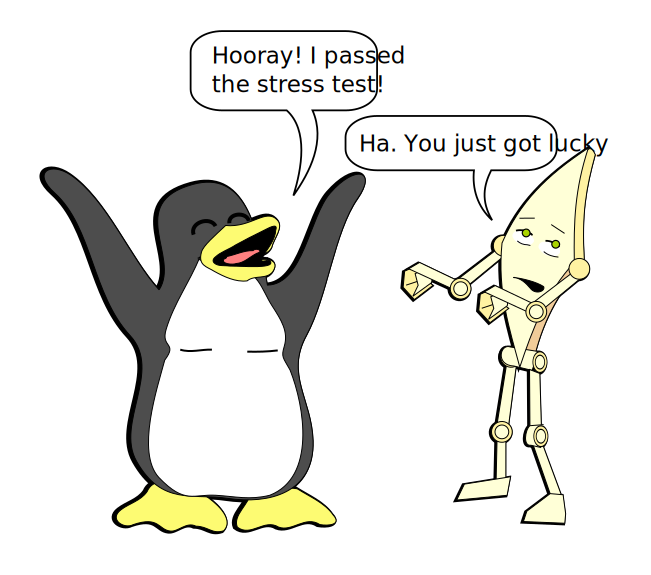
\includegraphics{cartoons/r-2014-Passed-the-stress-test}}
\caption{Passed on Merits?  Or Dumb Luck?}
\ContributedBy{Figure}{fig:cpu:Passed-the-stress-test}{Melissa Broussard}
\end{figure}

이제 질문은 버그가 발생하는 확률을 줄였거나, 관련된 버그들 중 하나만 고친
거이거나, 관계없는 무능한 변경을 만든게 아니고 여러분이 그 버그를 정말로
고쳤음을 확신하기 위해 얼마나 많은 테스트를 해야 하는지입니다.
짧게 말해서,
Figure~\ref{fig:cpu:Passed-the-stress-test} 의 영원한 질문에 대한 답은
무엇일까요?

불행히도, 솔직한 답은 완벽한 확신을 위해선 무한한 양의 테스트가 필요하다는
것입니다.

\iffalse

Now the question is just how much testing is required in order to be
certain that
you actually fixed the bug, as opposed to just reducing the probability
of it occurring on the one hand, having fixed only one of several
related bugs on the other hand, or made some ineffectual unrelated
change on yet a third hand.
In short, what is the answer to the eternal question posed by
Figure~\ref{fig:cpu:Passed-the-stress-test}?

Unfortunately, the honest answer is that an infinite amount of testing
is required to attain absolute certainty.

\fi

\QuickQuiz{
	여러분이 폐기할 수 있는 무척 많은 시스템을 가지고 있다고 해봅시다.
	예를 들어, 현재의 클라우드 가격대에서, 여러분은 낮은 가격으로 많은 CPU
	를 구매할 수 있습니다.
	모든 실용적 목적의 충분한 확실성을 위해 이 방법을 사용하는 건 어때요?

	\iffalse

	Suppose that you had a very large number of systems at your
	disposal.
	For example, at current cloud prices, you can purchase a
	huge amount of CPU time at low cost.
	Why not use this approach to get close enough to certainty
	for all practical purposes?

	\fi

}\QuickQuizAnswer{
	이 방법도 여러분의 검증 무기고에 가치있는 추가가 될 겁니다.
	하지만 ``모든 실용적 목적'' 을 불가능하게 하는 한계도 있습니다:
	\begin{enumerate}
	\item	어떤 버그는 극단적으로 낮은 발생확률을 가지지만 고쳐질 필요가
		없습니다.
		예를 들어, 리눅스 커널의 RCU 구현이 평균 백만년에 한번 발생하는
		버그를 가지고 있다고 해봅시다.
		백만년의 CPU 시간은 가장 싼 클라우드 플랫폼에서라 해도 굉장히
		비싸지만 2017년 기준 200억 개가 넘는 리눅스 인스턴스가 있으니
		하루에 50번도 넘는 실패가 발생할 거라 예상할 수 있습니다.
	\item	그 버그는 여러분의 특정 클라우드 컴퓨팅 테스트 환경에서는 발생
		확률이 0일 수도 있는데, 이는 여러분이 테스트에 얼마나 많은 기계
		시간을 사용하든 그걸 보지 못할 것을 의미합니다.
		한가지만 예를 들어보면, preemption 가능한 커널에서만 나타나는
		RCU 버그들이 있으며, preemption 불가능한 커널에서만 발생하는
		RCU 버그들도 있습니다.
	\end{enumerate}

	\iffalse

	This approach might well be a valuable addition to your
	validation arsenal.
	But it does have limitations that rule out ``for all practical
	purposes'':
	\begin{enumerate}
	\item	Some bugs have extremely low probabilities of occurrence,
		but nevertheless need to be fixed.
		For example, suppose that the Linux kernel's RCU
		implementation had a bug that is triggered only once
		per million years of machine time on average.
		A million years of CPU time is hugely expensive even on
		the cheapest cloud platforms, but we could expect
		this bug to result in more than 50 failures per day
		on the more than 20~billion Linux instances in the
		world as of 2017.
	\item	The bug might well have zero probability of occurrence
		on your particular cloud-computing test setup, which
		means that you won't see it no matter how much machine
		time you burn testing it.
		For but one example, there are RCU bugs that appear
		only in preemptible kernels, and also other RCU bugs
		that appear only in non-preemptible kernels.
	\end{enumerate}

	\fi

	물론, 여러분의 코드는 충분히 작아서
	Chapter~\ref{chp:Formal Verification} 에서 이야기하는 정형적 검증이
	도움이 될 겁니다.
	하지만 주의하세요: 여러분의 코드의 정형적 검증은 여러분의 가정,
	요구사항에 대한 오해, 여러분이 사용하는 소프트웨어 또는 하드웨어 기능에
	대한 오해, 혹은 여러분이 증명해야 할 것을 찾지 못한 오류에 대해서는
	오류를 찾지 못할겁니다.

	\iffalse

	Of course, if your code is small enough, formal validation
	may be helpful, as discussed in
	Chapter~\ref{chp:Formal Verification}.
	But beware: formal validation of your code will not find
	errors in your assumptions, misunderstanding of the
	requirements, misunderstanding of the software or hardware
	primitives you use, or errors that you did not think to construct
	a proof for.

	\fi

}\QuickQuizEnd

하지만 높은 확률을 선호해서 절대적 확실성을 포기하려 한다고 생각해 봅시다.
그럼 우린 강력한 통계 도구를 이 문제에 적용할 수 있습니다.
그러나, 이 섹션은 간단한 통계 도구들에 집중합니다.
이 도구들은 굉장히 도움이 되지만 이 섹션을 읽는게 통계 수업을 대체할 수는
없음을 알아두세요.\footnote{
	전 통계 수업을 강력히 추천합니다.
	제가 들었던 일부 통계 수업은 제가 수업 듣느라 쓴 시간보다 훨씬 많은
	가치를 제공했습니다.}

우리의 간단한 통계 도구를 시작하기 위해, 우린 개별 테스트를 할지 연속적
테스트를 할지 정해야 합니다.
개별 테스트는 잘 정의된 개별 테스트 수행들을 갖습니다.
예를 들어, 리눅스 커널 패치의 부팅 테스트는 개별 테스트의 한 예입니다:
커널은 부팅되거나 안되거나입니다.
여러분이 한시간동안 커널 부팅 테스트를 할 수 있더라도, 테스트를 수행하는데
사용한 시간보다 커널을 부팅하려 시도한 횟수와 부팅이 성공한 횟수에 더 관심있을
겁니다.
기능 테스트는 개별 테스트인 경향이 있습니다.

\iffalse

But suppose that we are willing to give up absolute certainty in favor
of high probability.
Then we can bring powerful statistical tools to bear on this problem.
However, this section will focus on simple statistical tools.
These tools are extremely helpful, but please note that reading this
section is not a substitute for statistics classes.\footnote{
	Which I most highly recommend.
	The few statistics courses I have taken have provided value
	far beyond that of the time I spent on them.}

For our start with simple statistical tools, we need to decide whether
we are doing discrete or continuous testing.
Discrete testing features well-defined individual test runs.
For example, a boot-up test of a Linux kernel patch is an example
of a discrete test:
The kernel either comes up or it does not.
Although you might spend an hour boot-testing your kernel, the number of
times you attempted to boot the kernel and the number of times the
boot-up succeeded would often be of more interest than the length
of time you spent testing.
Functional tests tend to be discrete.

\fi

반면에, 만약 제 패치가 RCU 에 관련되어 있다면, 저는 RCU 를 테스트하는 기묘한
커널 모듈인 \co{rcutorture} 를 아마 수행할겁니다.
개별 테스트의 성공적인 종료 시에 로그인 프롬프트 시그널을 보이는 커널 부팅과
달리, \co{rcutorture} 는 커널이 크래쉬 하거나 여러분이 멈추라고 하기 전까지 RCU
를 고문하길 계속할 겁니다.
\co{rcutorture} 테스트 시간은 여러분이 그걸 몇번이나 시작하고 종료했는지보다
관심있는 대상이 됩니다.
따라서, \co{rcutorture} 는 많은 스트레스 테스트를 포함하는 카테고리인 연속
테스트의 한 예입니다.

개별 테스트를 위한 통계는 더 간단하고 연속 테스트들보다 친숙하며, 개별 테스트를
위한 통계는 연속 테스트들을 위한 서비스에 사용될 수도 있는데, 정확도가 약간
떨어지긴 합니다.
따라서 개별 테스트부터 이야기를 시작해 봅시다.

\iffalse

On the other hand, if my patch involved RCU, I would probably run
\co{rcutorture}, which is a kernel module that, strangely enough, tests RCU\@.
Unlike booting the kernel, where the appearance of a login prompt
signals the successful end of a discrete test, \co{rcutorture} will happily
continue torturing RCU until either the kernel crashes or until you
tell it to stop.
The duration of the \co{rcutorture} test is usually of more
interest than the number of times you started and stopped it.
Therefore, \co{rcutorture} is an example of a continuous test, a category
that includes many stress tests.

Statistics for discrete tests are simpler and more familiar than those
for continuous tests, and furthermore the statistics for discrete tests
can often be pressed into service for continuous tests, though with some
loss of accuracy.
We therefore start with discrete tests.

\fi

\subsection{Statistics for Discrete Testing}
\label{sec:debugging:Statistics for Discrete Testing}

어떤 버그가 한번 수행시 10\,\% 발생확률을 가지며 우리가 다섯번 수행한다고
해봅시다.
그 중 최소 한번의 수행은 실패할 확률을 어떻게 계산할까요?
여기 한가지 방법이 있습니다:

\iffalse

Suppose a bug has a 10\,\% chance of occurring in a given run and that
we do five runs.
How do we compute the probability of at least one run failing?
Here is one way:

\fi

\begin{enumerate}
\item	특정 수행이 성공할 확률, 90\,\% 를 계산합니다.
\item	다섯번의 수행이 모두 성공할 확률, 0.9 를 다섯번 곱한 값, 약 59\,\% 를
	계산합니다.
\item	모든 다섯번의 수행이 성공하거나 최소 한번은 실패하거나 이므로 예상된
	성공 확률은 59\,\% 를 100\,\% 에서 빼서 41\,\% 의 실패 확률을
	도출합니다.

\iffalse

\item	Compute the probability of a given run succeeding, which is 90\,\%.
\item	Compute the probability of all five runs succeeding, which
	is 0.9 raised to the fifth power, or about 59\,\%.
\item	Because either all five runs succeed, or at least one fails,
	subtract the 59\,\% expected success rate from 100\,\%, yielding
	a 41\,\% expected failure rate.

\fi

\end{enumerate}

수식을 선호하는 사람들을 위해, 한번 실패할 확률을 $f$ 라 합시다.
한번 성공할 확률은 그러면 $1-f$ 이며 모든 $n$ 테스트가 성공할 확률은 $S_n$
입니다:

\iffalse

For those preferring formulas, call the probability of a single failure $f$.
The probability of a single success is then $1-f$ and the probability
that all of $n$ tests will succeed is $S_n$:

\fi

\begin{equation}
	S_n = \left(1-f\right)^n
\end{equation}

실패할 확률은 $1-S_n$, 또는:

\iffalse

The probability of failure is $1-S_n$, or:

\fi

\begin{equation}
	F_n = 1-\left(1-f\right)^n
\label{eq:debugging:Binomial Failure Rate}
\end{equation}

\QuickQuiz{
	뭐라구요???
	앞의 10\,\% 실패율의 다섯번의 테스트 예를 이 식에 대입해보면 59,050\,\%
	를 얻게 되는데 이건 말이 안되잖아요!!!

	\iffalse

	Say what???
	When I plug the earlier five-test 10\,\%-failure-rate example into
	the formula, I get 59,050\,\% and that just doesn't make sense!!!

	\fi

}\QuickQuizAnswer{
	그 말이 맞습니다, 말이 안되죠.

	확률은 0과 1 사이의 수여서 확률을 구하기 위해선 퍼센트 값을 100 으로
	나눠야 함을 기억하세요.
	따라서 10\,\% 는 0.1 의 확률이며, 0.4095, 반올림해 41\,\% 의 확률을
	얻게 되는데 앞의 결과와 잘 들어맞습니다.

	\iffalse

	You are right, that makes no sense at all.

	Remember that a probability is a number between zero and one,
	so that you need to divide a percentage by 100 to get a
	probability.
	So 10\,\% is a probability of 0.1, which gets a probability
	of 0.4095, which rounds to 41\,\%, which quite sensibly
	matches the earlier result.

	\fi

}\QuickQuizEnd

어떤 테스트가 10\,\% 회 실패했다고 가정해 봅시다.
여러분의 수정이 정말 도움이 되었음을 99\,\% 확신하려면 얼마나 많이 테스트를
반복해야 할까요?

이 질문을 묻는 다른 방법은 ``실패 확률이 99\,\% 까지 오르게 하려면 몇번이나
테스트를 수행해야 할까요?'' 입니다.
어쨌건, 한번이라도 실패를 보게 될 확률이 99\,\% 이기 충분할 정도로 테스트를
반복한다면, 그리고 거기서 실패를 보지 못했다면, 이 ``성공'' 이 행운 덕일 뿐일
확률은 1\,\% 뿐입니다.
그리고
Equation~\ref{eq:debugging:Binomial Failure Rate} 에 $f=0.1$ 을 넣고 $n$ 을
변화시켜보면, 테스트 수행당 10\,\% 실패 확률을 갖는 상황에서 최소 한번은 실패할
확률은 43회 수행에서 98.92\,\%, 44회 수행에서 99.03\,\% 가 됩니다.
그러니 우리의 수정사항을 포함한 테스트 수행이 44회 반복해서 실패하지 않는다면
우리의 수정사항이 정말로 도움이 되었을 확률이 99\,\% 가 됩니다.

하지만 반복적으로
Equation~\ref{eq:debugging:Binomial Failure Rate} 에 수를 넣는 건 지루할 수
있으니, $n$ 을 풀어봅시다:

\iffalse

So suppose that a given test has been failing 10\,\% of the time.
How many times do you have to run the test to be 99\,\% sure that
your supposed fix actually helped?

Another way to ask this question is ``How many times would we need
to run the test to cause the probability of failure to rise above 99\,\%?''
After all, if we were to run the test enough times that the probability
of seeing at least one failure becomes 99\,\%, if there are no failures,
there is only 1\,\% probability of this ``success'' being due to dumb luck.
And if we plug $f=0.1$ into
Equation~\ref{eq:debugging:Binomial Failure Rate} and vary $n$,
we find that 43 runs gives us a 98.92\,\% chance of at least one test failing
given the original 10\,\% per-test failure rate,
while 44 runs gives us a 99.03\,\% chance of at least one test failing.
So if we run the test on our fix 44 times and see no failures, there
is a 99\,\% probability that our fix really did help.

But repeatedly plugging numbers into
Equation~\ref{eq:debugging:Binomial Failure Rate}
can get tedious, so let's solve for $n$:

\fi

\begin{eqnarray}
	F_n = 1-\left(1-f\right)^n \\
	1 - F_n = \left(1-f\right)^n \\
	\log \left(1 - F_n\right) = n \; \log \left(1 - f\right)
\end{eqnarray}

마지막으로 필요한 테스트 횟수는 다음과 같이 됩니다:

\iffalse

Finally the number of tests required is given by:

\fi

\begin{equation}
	n = \frac{\log\left(1 - F_n\right)}{\log\left(1 - f\right)}
\label{eq:debugging:Binomial Number of Tests Required}
\end{equation}

Equation~\ref{eq:debugging:Binomial Number of Tests Required}
에 $f=0.1$ 과 $F_n=0.99$ 를 대입하면 43.7 이 나오는데, 우리의 수정사항이 정말
개선을 만들었음에 99\,\% 자신하려면 44번의 연속된 테스트 성공이 있어야 함을
의미합니다.
이는 앞의 방법으로 얻어진 수와 일치하므로, 안심해도 되겠습니다.

\iffalse

Plugging $f=0.1$ and $F_n=0.99$ into
Equation~\ref{eq:debugging:Binomial Number of Tests Required}
gives 43.7, meaning that we need 44 consecutive successful test
runs to be 99\,\% certain that our fix was a real improvement.
This matches the number obtained by the previous method, which
is reassuring.

\fi

\QuickQuiz{
	Equation~\ref{eq:debugging:Binomial Number of Tests Required} 에서,
	로그의 밑은 10인가요, 2인가요, 아니면 $\euler$ 인가요?

	\iffalse

	In Equation~\ref{eq:debugging:Binomial Number of Tests Required},
	are the logarithms base-10, base-2, or base-$\euler$?

	\fi

}\QuickQuizAnswer{
	상관없습니다.
	이 결과는 로그값 사이의 비율이므로 어떤 밑을 사용하더라도 같은 답을
	얻게 됩니다.
	유일한 제약은 여러분이 분자와 분모에 모두 같은 밑을 사용해야 한다는
	겁니다.

	\iffalse

	It does not matter.
	You will get the same answer no matter what base of logarithms
	you use because the result is a pure ratio of logarithms.
	The only constraint is that you use the same base for both
	the numerator and the denominator.

	\fi

}\QuickQuizEnd

\begin{figure}[tb]
\centering
\resizebox{2.5in}{!}{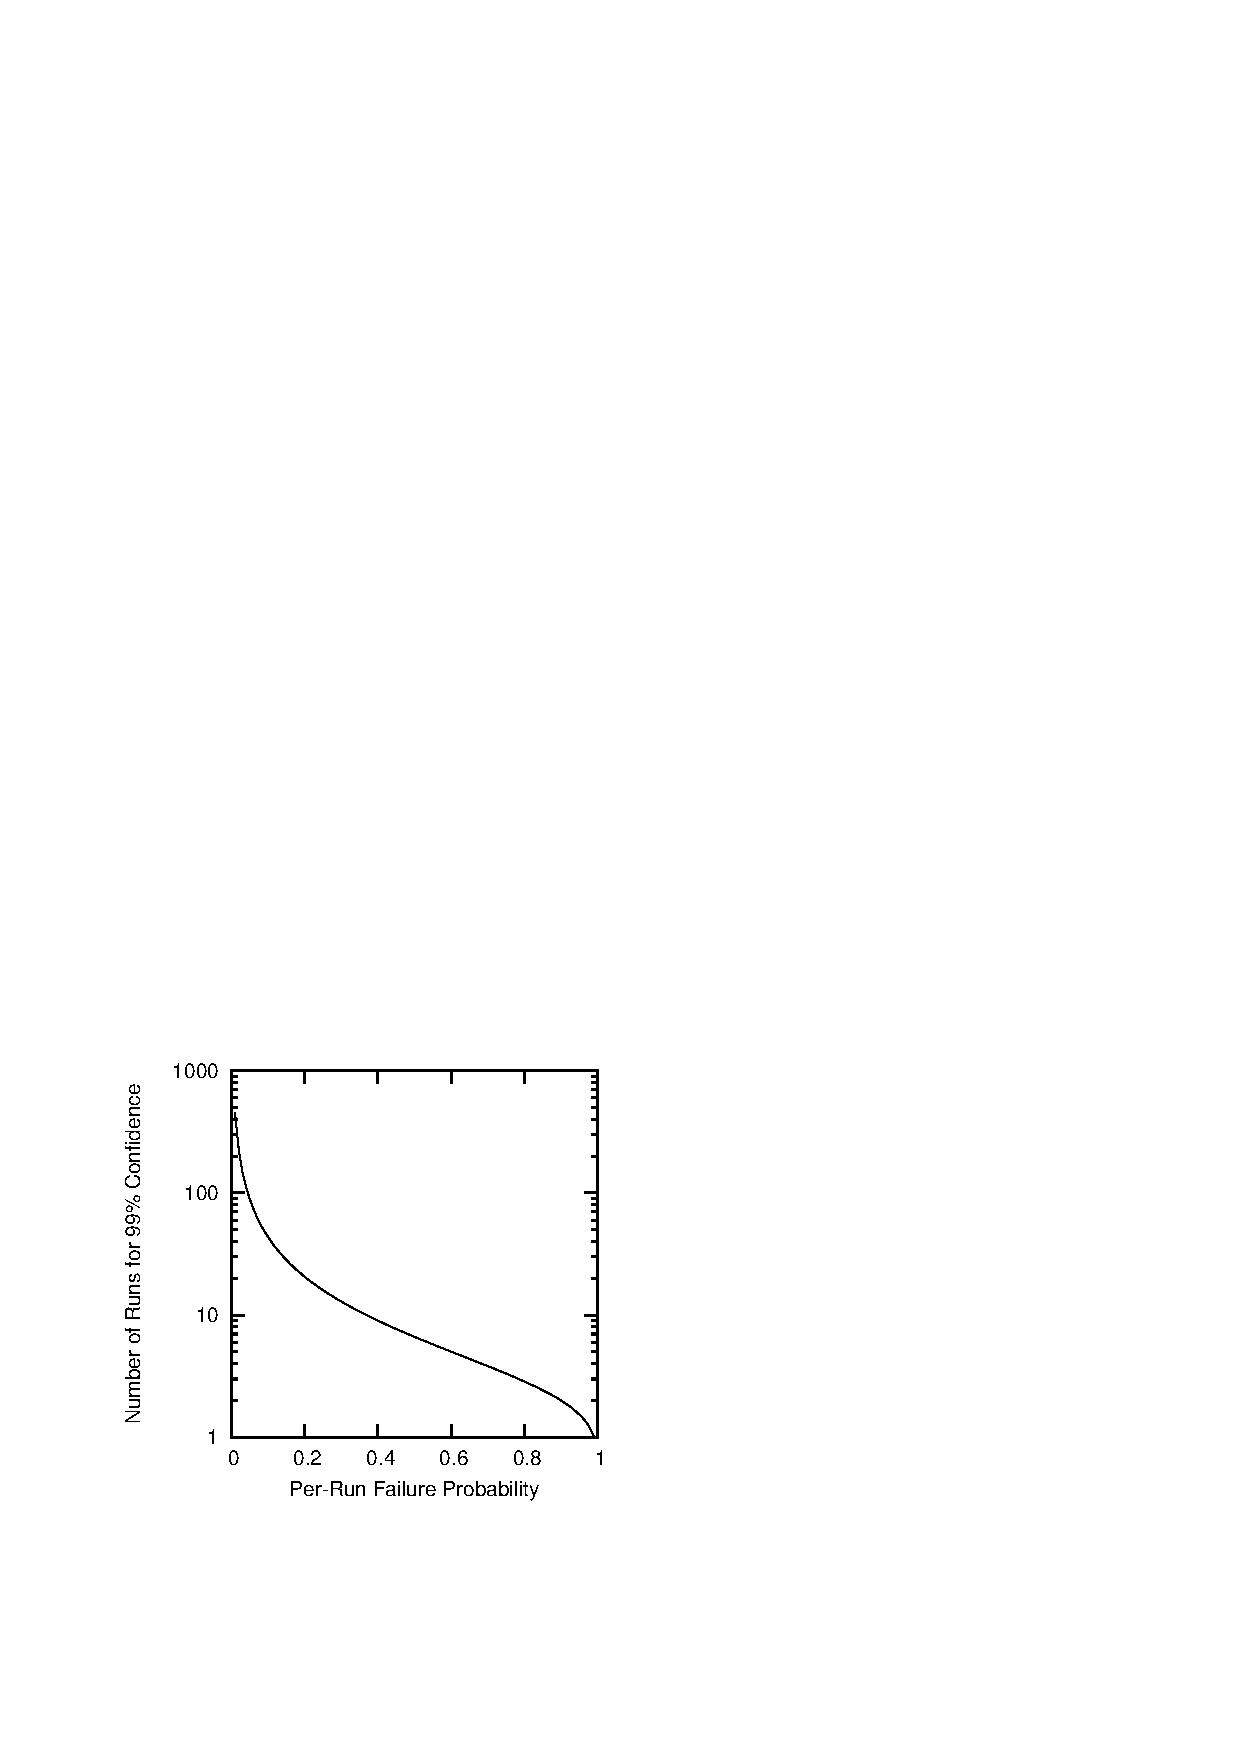
\includegraphics{CodeSamples/debugging/BinomialNRuns}}
\caption{Number of Tests Required for 99 Percent Confidence Given Failure Rate}
\label{fig:debugging:Number of Tests Required for 99 Percent Confidence Given Failure Rate}
\end{figure}

Figure~\ref{fig:debugging:Number of Tests Required for 99 Percent Confidence Given Failure Rate}
가 이 함수의 그림을 보입니다.
놀랍지 않게도, 덜 빈번하게 각 테스트가 실패할수록, 버그가 고쳐졌다고 99\,\%
확신하는데 필요한 테스트 수행 횟수가 늘어납니다.
이 버그가 1\,\% 의 테스트에서만 실패한다면, 458 회의 테스트가 필요합니다.
실패 확률이 줄어들수록, 필요한 테스트 횟수는 늘어나서, 실패 확률이 0이 되면
무한대가 됩니다.

이 이야기의 교훈은 여러분이 드물게 발생하는 버그를 찾았을 때, 여러분이 조심스레
만들어져 훨씬 높은 실패 확률을 갖는 테스트를 사용할 때 여러분의 테스트 업무가
훨씬 쉬워질 것이라는 겁니다.
예를 들어, 여러분의 테스트가 실패 확률을 1\,\% 에서 30\,\% 로 늘린다면 99\,\%
확신을 위한 테스트 횟수는 458 에서 13 으로 떨어집니다.

\iffalse

Figure~\ref{fig:debugging:Number of Tests Required for 99 Percent Confidence Given Failure Rate}
shows a plot of this function.
Not surprisingly, the less frequently each test run fails, the more
test runs are required to be 99\,\% confident that the bug has been
fixed.
If the bug caused the test to fail only 1\,\% of the time, then a
mind-boggling 458 test runs are required.
As the failure probability decreases, the number of test runs required
increases, going to infinity as the failure probability goes to zero.

The moral of this story is that when you have found a rarely occurring
bug, your testing job will be much easier if you can come up with
a carefully targeted test with a much higher failure rate.
For example, if your targeted test raised the failure rate from 1\,\%
to 30\,\%, then the number of runs required for 99\,\% confidence
would drop from 458 to a more tractable 13.

\fi

하지만 이 13회 테스트 수행은 여러분의 수정이 ``어떤 개선'' 을 만들었다는 99\,\%
자신감만을 줍니다.
여러분의 수정 사항이 실패 확률을 열배 줄였다는 자신감을 99\,\% 얻고자 한다고
해봅시다.
얼마나 많은 테스트 성공 횟수가 필요할까요?

30\,\% 실패 확률에서 열배 개선이면 3\,\% 실패 확률일 겁니다.
이를
Equation~\ref{eq:debugging:Binomial Number of Tests Required} 에 대입하면:

\iffalse

But these thirteen test runs would only give you 99\,\% confidence that
your fix had produced ``some improvement''.
Suppose you instead want to have 99\,\% confidence that your fix reduced
the failure rate by an order of magnitude.
How many failure-free test runs are required?

An order of magnitude improvement from a 30\,\% failure rate would be
a 3\,\% failure rate.
Plugging these numbers into
Equation~\ref{eq:debugging:Binomial Number of Tests Required} yields:

\fi

\begin{equation}
	n = \frac{\log\left(1 - 0.99\right)}{\log\left(1 - 0.03\right)} = 151.2
\end{equation}

따라서 열배 개선은 대략 열배 더 많은 테스트를 필요로 합니다.
확정성은 불가능하며, 높은 확률은 매우 비쌉니다.
이것이 테스트가 더 빠르게 수행되고 실패가 잘 발생하게 하는게 고도로 안정화된
소프트웨어를 개발하는데 필수의 기술인지에 대한 이유입니다.
이 기술들은
Section~\ref{sec:debugging:Hunting Heisenbugs} 에서 다루어집니다.

\iffalse

So our order of magnitude improvement requires roughly an order of
magnitude more testing.
Certainty is impossible, and high probabilities are quite expensive.
This is why making tests run more quickly and making failures more
probable are essential skills in the development of highly reliable
software.
These skills will be covered in
Section~\ref{sec:debugging:Hunting Heisenbugs}.

\fi

\subsection{Statistics Abuse for Discrete Testing}
\label{sec:debugging:Statistics Abuse for Discrete Testing}

하지만 열시간마다 약 세번 실패하는 반복적 테스트가 있고, 그 실패를 유발했다고
여겨지는 버그를 고쳤다고 해봅시다.
여러분이 실패 확률을 줄였음에 99\,\% 자신하기 위해선 이 테스트를 실패 없이
얼마나 오래 수행해야 할까요?

통계에 상당한 폭력을 가하지 않고, 우린 한시간 수행을 30\,\% 실패 확률을 갖는
개별 테스트로 재정의 할 수 있습니다.
그러면 앞의 섹션에서의 결과가 그 테스트가 13시간동안 실패 없이 수행된다면
우리의 수정사항이 이 프로그램의 안정성을 정말 개선했다는 99\,\% 자신을 가질 수
있다고 합니다.

독실한 확률가는 이 방법을 허락하지 않을 것이지만, 슬픈 사실은 이런 종류의 확률
남용에 의한 오류들은 여러분의 실패 확률 예측 상의 오류에 비하면 무척 작다는
겁니다.
그러나, 다음 섹션은 더 엄격한 방법을 알아봅니다.

\iffalse

But suppose that you have a continuous test that fails about three
times every ten hours, and that you fix the bug that you believe was
causing the failure.
How long do you have to run this test without failure to be 99\,\% certain
that you reduced the probability of failure?

Without doing excessive violence to statistics, we could simply
redefine a one-hour run to be a discrete test that has a 30\,\%
probability of failure.
Then the results of in the previous section tell us that if the test
runs for 13 hours without failure, there is a 99\,\% probability that
our fix actually improved the program's reliability.

A dogmatic statistician might not approve of this approach, but the sad
fact is that the errors introduced by this sort of statistical abuse are
usually quite small compared to the errors in your failure-rate estimates.
Nevertheless, the next section takes a more rigorous approach.

\fi

\subsection{Statistics for Continuous Testing}
\label{sec:debuggingStatistics for Continuous Testing}

실패 확률의 기본 공식은 Poisson 분포입니다:

\iffalse

The fundamental formula for failure probabilities is the Poisson
distribution:

\fi

\begin{equation}
	F_m = \frac{\lambda^m}{m!} \euler^{-\lambda}
\label{eq:debugging:Poisson Probability}
\end{equation}

여기서 $F_m$ 은 테스트에서 $m$ 회 실패할 확률이며 $\lambda$ 는 단위 시간당
예상되는 실패율입니다.
모든 고급 확률 교재에서는 상당한 도출이 있겠는데, 예를들어 Feller 의 고전인
``An Introduction to Probability Theory and Its Applications''~\cite{Feller58}
이 있겠으며, 더 직관적인 도출은 이 책의 첫번째
판본에서~\cite[Equations 11.8--11.26]{McKenney2014ParallelProgramming-e1}
찾아볼 수 있을 겁니다.

Section~\ref{sec:debugging:Statistics Abuse for Discrete Testing}
의 예를 Possion 분포를 사용해 다시 작업해 봅시다.
이 예는 시간당 30\,\% 실패율을 갖는 테스트를 사용하며 질문은 수정이 실패 확률을
줄였음을 99\,\% 확신하기 위해 얼마나 오래 에러 없이 테스트를 돌려야
하는지임을 다시 말씀드립니다.
이 경우, $m$ 은 0이며, 따라서 Equation~\ref{eq:debugging:Poisson Probability}
은 다음과 같이 요약됩니다:

\iffalse

Here $F_m$ is the probability of $m$ failures in the test and
$\lambda$ is the expected failure rate per unit time.
A rigorous derivation may be found in any advanced probability
textbook, for example, Feller's classic ``An Introduction to Probability
Theory and Its Applications''~\cite{Feller58}, while a more
intuitive derivation may be found in the first edition of
this book~\cite[Equations 11.8--11.26]{McKenney2014ParallelProgramming-e1}.

Let's try reworking the example from
Section~\ref{sec:debugging:Statistics Abuse for Discrete Testing}
using the Poisson distribution.
Recall that this example involved a test with a 30\,\% failure rate per
hour, and that the question was how long the test would need to run
error-free
on a alleged fix to be 99\,\% certain that the fix actually reduced the
failure rate.
In this case, $m$ is zero, so that
Equation~\ref{eq:debugging:Poisson Probability} reduces to:

\fi

\begin{equation}
	F_0 =  \euler^{-\lambda}
\end{equation}

이를 푸는데는 $F_0$ 를 0.01 로 하고 $\lambda$ 를 구할 것이 필요해지는데, 다음과
같습니다:

\iffalse

Solving this requires setting $F_0$
to 0.01 and solving for $\lambda$, resulting in:

\fi

\begin{equation}
	\lambda = - \ln 0.01 = 4.6
\end{equation}

시간당 $0.3$ 실패를 가지므로, 필요한 시간은 $4.6/0.3 = 14.3$ 로,
Section~\ref{sec:debugging:Statistics Abuse for Discrete Testing} 에서의
방법으로 계산된 13 시간의 10\,\% 입니다.
보통 여러분의 실패 확률이 10\,\% 근처임을 모를 것을 놓고 생각하면,
Section~\ref{sec:debugging:Statistics Abuse for Discrete Testing}
에서 이야기된 더 간단한 방법이 거의 항상 충분히 좋을 겁니다.

더 일반적으로는, 만약 우리가 단위 시간당 $n$ 회 실패를 한다면, 그리고 어떤
수정사항이 이 실패 확률을 줄였음을 $P$\,\% 확신하려면 다음 공식을 사용할 수
있습니다:

\iffalse

Because we get $0.3$ failures per hour, the number of hours required
is $4.6/0.3 = 14.3$, which is within 10\,\% of the 13 hours
calculated using the method in
Section~\ref{sec:debugging:Statistics Abuse for Discrete Testing}.
Given that you normally won't know your failure rate to anywhere near
10\,\%, the simpler method described in
Section~\ref{sec:debugging:Statistics Abuse for Discrete Testing}
is almost always good and sufficient.

More generally, if we have $n$ failures per unit time, and we want to
be $P$\,\% certain that a fix reduced the failure rate, we can use the
following formula:

\fi

\begin{equation}
	T = - \frac{1}{n} \ln \frac{100 - P}{100}
\label{eq:debugging:Error-Free Test Duration}
\end{equation}

\QuickQuiz{
	어떤 버그가 어떤 테스트를 시간당 평균 세번 실패를 하게 한다고 해봅시다.
	어떤 수정사항이 그 실패 확률을 충분히 줄였음을 99.9\,\% 확신하기 위해선
	얼마나 오래 에러 없는 테스트 수행을 해야 할까요?

	\iffalse

	Suppose that a bug causes a test failure three times per hour
	on average.
	How long must the test run error-free to provide 99.9\,\%
	confidence that the fix significantly reduced the probability
	of failure?

	\fi

}\QuickQuizAnswer{
	Equation~\ref{eq:debugging:Error-Free Test Duration} 에 $n$ 을 $3$
	으로, $P$ 를 $99.9$ 로 하면 다음과 같이 됩니다:

	\iffalse

	We set $n$ to $3$ and $P$ to $99.9$ in
	Equation~\ref{eq:debugging:Error-Free Test Duration}, resulting in:

	\fi

	\begin{equation}
		T = - \frac{1}{3} \ln \frac{100 - 99.9}{100} = 2.3
	\end{equation}

	테스트가 실패 없이 2.3 시간을 수행된다면 우린 이 수정사항이 실패 확률을
	줄였음을 99.9\,\% 확신할 수 있습니다.

	\iffalse

	If the test runs without failure for 2.3 hours, we can be 99.9\,\%
	certain that the fix reduced the probability of failure.

	\fi

}\QuickQuizEnd

이전과 같이, 버그가 덜 빈번히 발생하고 필요한 확신의 수준이 높을수록 에러 없는
테스트 수행은 더 길게 필요해집니다.

어떤 테스트가 시간당 한번 정도 실패하지만 어떤 버그 수정 후, 24시간의
테스트에서 두번만 실패한다고 해봅시다.
이 버그로 이끄는 실패가 무작위적으로 발생한다고 가정하면, 두번째 수행에서의
적은 수의 실패가 무작위적 선택에 의한 것일 확률이 얼마나 될까요?
달리 말하자면, 그 수정이 버그에 영향을 줬음에 우린 얼마나 자신할 수 있을까요?
이 확률은
Equation~\ref{eq:debugging:Poisson Probability} 을 다음과 가이 더해서 계산할 수
있을 겁니다:

\iffalse

As before, the less frequently the bug occurs and the greater the
required level of confidence, the longer the required error-free test run.

Suppose that a given test fails about once every hour, but after a bug
fix, a 24-hour test run fails only twice.
Assuming that the failure leading to the bug is a random occurrence,
what is the probability that the small number of
failures in the second run was due to random chance?
In other words, how confident should we be that the fix actually
had some effect on the bug?
This probability may be calculated by summing
Equation~\ref{eq:debugging:Poisson Probability} as follows:

\fi

\begin{equation}
	F_0 + F_1 + \dots + F_{m - 1} + F_m =
		\sum_{i=0}^m \frac{\lambda^i}{i!} \euler^{-\lambda}
\end{equation}

이는 다음과 같이 요약될 수 있는 Poisson 누적 분포 함수입니다:

\iffalse

This is the Poisson cumulative distribution function, which can be
written more compactly as:

\fi

\begin{equation}
	F_{i \le m} = \sum_{i=0}^m \frac{\lambda^i}{i!} \euler^{-\lambda}
\label{eq:debugging:Possion CDF}
\end{equation}

여기서 $m$ 은 긴 시간의 테스트 수행 (이 경우, 두시간) 에서의 오류 횟수이며
$\lambda$ 는 긴 테스트 수행에서 (이 경우 ,24시간) 예상되는 오류의 수입니다.
$m=2$ 와 $\lambda=24$ 를 이 식에 대입하면 두번 이하 실패 확률은 $1.2 \times
10^{-8}$ 이 되는데, 달리 말하면 이 수정이 버그에 어떤 영향을 주었다는 높은
수준의 자신을 가질 수 있습니다.\footnote{
	물론, 이는 여러분이 남은 두번의 실패를 초래한 버그(들)을 찾아서 고쳐야
	한다는데에 대한 변명이 되지 않습니다!}

\iffalse

Here $m$ is the actual number of errors in the long test run
(in this case, two) and $\lambda$ is expected number of errors
in the long test run (in this case, 24).
Plugging $m=2$ and $\lambda=24$ into this expression gives the probability
of two or fewer failures as about
$1.2 \times 10^{-8}$, in other words, we have a high level of confidence
that the fix actually had some relationship to the bug.\footnote{
	Of course, this result in no way excuses you from finding and
	fixing the bug(s) resulting in the remaining two failures!}

\fi

\QuickQuizSeries{%
\QuickQuizB{
	이 모든 factorial 과 exponential 을 더하는 건 고통입니다.
	더 쉬운 방법은 없나요?

	\iffalse

	Doing the summation of all the factorials and exponentials
	is a real pain.
	Isn't there an easier way?

	\fi

}\QuickQuizAnswerB{
	한가지 방법은 ``maxima'' 라는 오픈소스 기호 조작 프로그램을 사용하는
	겁니다.
	많은 리눅스 배포판의 일부인 이 프로그램을 설치하면 여러분은 그걸
	실행하고
	\co{load(distrib);} 에 이어 여러
	\co{bfloat(cdf_poisson(m,l));} 커맨드를 사용할 수 있는데, \co{m} 은
	원하는 $m$ 값으로 교체하고 (실제 테스트에서의 실제 실패 횟수) \co{l} 은
	원하는 $\lambda$ (실제 테스트에서 예상되는 실패 횟수) 로 설정해야
	합니다.

	특히, \co{bfloat(cdf_poisson(2,24));} 커맨드는
	\co{1.181617112359357b-8} 가 되는데,
	Equation~\ref{eq:debugging:Possion CDF} 에서의 값과 일치합니다.

	\iffalse

	One approach is to use the open-source symbolic manipulation
	program named ``maxima''.
	Once you have installed this program, which is a part of many
	Linux distributions, you can run it and give the
	\co{load(distrib);} command followed by any number of
	\co{bfloat(cdf_poisson(m,l));} commands, where the \co{m} is
	replaced by the desired value of $m$ (the actual number of failures in
	actual test) and the \co{l} is replaced by the desired value of
	$\lambda$ (the expected number of failures in the actual test).

	In particular, the \co{bfloat(cdf_poisson(2,24));} command
	results in \co{1.181617112359357b-8}, which matches the value
	given by Equation~\ref{eq:debugging:Possion CDF}.

	\fi

\begin{table}[tb]
\renewcommand*{\arraystretch}{1.25}
\rowcolors{3}{}{lightgray}
\small
\centering
\begin{tabular}{rrrr}
	\toprule
		& \multicolumn{3}{c}{Improvement} \\
		\cmidrule(l){2-4}
	Certainty (\%)
		& Any
			& 10x
				& 100x \\
	\cmidrule{1-1} \cmidrule(l){2-4}
	90.0	& 2.3	& 23.0	& 230.0  \\
	95.0	& 3.0	& 30.0	& 300.0  \\
	99.0	& 4.6	& 46.1	& 460.5  \\
	99.9	& 6.9	& 69.1	& 690.7  \\
	\bottomrule
\end{tabular}
\caption{Human-Friendly Poisson-Function Display}
\label{tab:debugging:Human-Friendly Poisson-Function Display}
\end{table}

	다른 방법은 이 실제 세계를 인정하는 것으로, 349.2x 안정성 개선의
	76.8\,\% 확신을 주기 위해 두번 이하의 오류를 테스트 기간을 계산하는게
	전혀 유용하지 않다는 것입니다.
	대신, 인간은 특정 값에 집중하려 하는데, 예를 들어 10x 개선의 95\,\%
	확신입니다.
	사람들은 또한 오류가 없는 테스트 수행을 훨씬 선호하는데 그게 여러분에게
	필요한 테스트 시간을 줄이므로 여러분도 그럴겁니다.
	따라서,
	\cref{tab:debugging:Human-Friendly Poisson-Function Display}
	의 값들이 충분한 겨우가 많을 겁니다.
	간단히 원하는 확신도와 개선 정도를 찾아보면 그 결과 숫자가 한번의
	오류가 나타나기 위해 예상되는 시간을 위한 에러 없는 테스트 시간을 보일
	겁니다.
	따라서 여러분의 수정 전 테스트가 시간당 한번의 실패를 겪었다면, 10x
	개선의 95\,\% 확신을 갖기 위해 여러분은 30시간의 오류 없는 테스트
	수행을 해야 합니다.

	대안적으로, 여러분은
	Section~\ref{sec:debugging:Statistics Abuse for Discrete Testing}
	에 소개된 대략적이고 준비된 방법을 사용할 수 있습니다.

	\iffalse

	Another approach is to recognize that in this real world,
	it is not all that useful to compute (say) the duration of a test
	having two or fewer errors that would give a 76.8\,\% confidence
	of a 349.2x improvement in reliability.
	Instead, human beings tend to focus on specific values, for
	example, a 95\,\% confidence of a 10x improvement.
	People also greatly prefer error-free test runs, and so should
	you because doing so reduces your required test durations.
	Therefore, it is quite possible that the values in
	\cref{tab:debugging:Human-Friendly Poisson-Function Display}
	will suffice.
	Simply look up the desired confidence and degree of improvement,
	and the resulting number will give you the required
	error-free test duration in terms of the expected time for
	a single error to appear.
	So if your pre-fix testing suffered one failure per hour, and the
	powers that be require a 95\,\% confidence of a 10x improvement,
	you need a 30-hour error-free run.

	Alternatively, you can use the rough-and-ready method described in
	Section~\ref{sec:debugging:Statistics Abuse for Discrete Testing}.

	\fi

}\QuickQuizEndB
%
\QuickQuizE{
	하지만 기다려요!!!
	\emph{약간의} 실패가 있음을 생각하면 (0번 실패할 확률을 포함해),
	Equation~\ref{eq:debugging:Possion CDF} 은 $m$ 이 무한으로 감에 따라
	$1$ 의 값이 되지 않나요?

	\iffalse

	But wait!!!
	Given that there has to be \emph{some} number of failures
	(including the possibility of zero failures), shouldn't
	Equation~\ref{eq:debugging:Possion CDF}
	approach the value $1$ as $m$ goes to infinity?

	\fi

}\QuickQuizAnswerE{
	맞습니다.
	그리고 그렇습니다.

	이걸 자세히 보기 위해, 
	 $\euler^{-\lambda}$ 는 $i$ 에 의존하지 않는데 이는 다음과 같이 합으로
	 나올 수 있음에 주목하시기 바랍니다:

	 \iffalse

	Indeed it should.
	And it does.

	To see this, note that $\euler^{-\lambda}$ does not depend on $i$,
	which means that it can be pulled out of the summation as follows:

	\fi

	\begin{equation}
		\euler^{-\lambda} \sum_{i=0}^\infty \frac{\lambda^i}{i!}
	\end{equation}

	남아있는 합은 $\euler^\lambda$ 의 Taylor 시리즈여서 다음이 도출됩니다:

	\iffalse

	The remaining summation is exactly the Taylor series for
	$\euler^\lambda$, yielding:

	\fi

	\begin{equation}
		\euler^{-\lambda} \euler^\lambda
	\end{equation}

	이 두 exponential 은 상흥하는 것이며, 따라서 취소될 수 있어서
	필요한대로 정확히 $1$ 이 됩니다.

	\iffalse

	The two exponentials are reciprocals, and therefore cancel,
	resulting in exactly $1$, as required.

	\fi

}\QuickQuizEndE
}

Poisson 분포는 테스트 결과를 분석하기 위한 강력한 도구입니다만 이 마지막
예에서는 여전히 24시간 테스트 수행에서의 두번의 실패가 남아있었음이 사실입니다.
그런 낮은 실패 확률은 매우 긴 테스트 수행을 초래합니다.
다음 섹션은 이 상황을 개선하는 반직관적인 방법들을 이야기 합니다.

\iffalse

The Poisson distribution is a powerful tool for analyzing test results,
but the fact is that in this last example there were still two remaining
test failures in a 24-hour test run.
Such a low failure rate results in very long test runs.
The next section discusses counter-intuitive ways of improving this situation.

\fi

\subsection{Hunting Heisenbugs}
\label{sec:debugging:Hunting Heisenbugs}

이 생각은 또한 heisenbug 의 설명을 돕습니다:
추적과 단정을 더하는 것은 버그가 나타나는 확률을 쉽게 줄이는데, 극단적으로
가벼운 추적과 단정 메커니즘이 치명적으로 중요한 이유이다.

``Heisenbug'' 라는 용어는 특정 입자의 특정 시간에서의 위치와 속도를 정확하게
알아내는 것은 불가능하다고 이야기하는 \pplsur{Weiner}{Heisenberg} 의
\IX{Uncertainty Principle} (불확정성 원리)~\cite{WeinerHeisenberg1927Uncertain}
에 영감을 받아 만들어졌습니다.
어떤 입자의 위치를 정확하게 측정하려는 모든 시도는 그것의 속도의 불확정성을
증가시키며 그 반대 역시 마찬가지입니다.
비슷하게, heisenbug 를 추적하려는 시도는 그 증상이 크게 바뀌거나 심지어 완전히
사라지게도 만듭니다.\footnote{
	``Heisenbug'' 라는 용어는 잘못된 호칭인데, 대부분의 heisenbug 는 고전
	물리학의 \emph{observer effect} 로 설명되기 때문입니다.
	그러나, 그 이름은 유행하지 못했습니다.}

\iffalse

This line of thought also helps explain heisenbugs:
adding tracing and assertions can easily reduce the probability
of a bug appearing, which
is why extremely lightweight tracing and assertion mechanism are
so critically important.

The term ``heisenbug'' was inspired by the \pplsur{Weiner}{Heisenberg}
\IX{Uncertainty Principle} from quantum physics, which states that
it is impossible to
exactly quantify a given particle's position and velocity at any given
point in time~\cite{WeinerHeisenberg1927Uncertain}.
Any attempt to more accurately measure that particle's position will
result in increased uncertainty of its velocity and vice versa.
Similarly, attempts to track down
the heisenbug causes its symptoms to radically change or even disappear
completely.\footnote{
	The term ``heisenbug'' is a misnomer, as most heisenbugs are
	fully explained by the \emph{observer effect} from classical
	physics.
	Nevertheless, the name has stuck.}

\fi

만약 해당 물리학계가 이 문제의 이름에 영감을 주었다면, 해당 물리학계가 그
해법에도 영감을 주는게 공평합니다.
다행히도, 입자 물리학은 그 일을 하고 있습니다:
Heisenbug 를 무효화 시키기 위해 anti-heisenbug 를 만드는 게 어떻습니까?
또는, 아마 더 정확히는, heisenbug 의 heisen 특성을 무효화 시키기 위해?
특정 heisenbug 를 위한 anti-heisenbug 를 만드는 것은 과학보다는 예술의
영역인데, 다음 섹션들이 그걸 하기 위한 방법들을 설명합니다:

\iffalse

If the field of physics inspired the name of this problem, it is only
fair that the field of physics should inspire the solution.
Fortunately, particle physics is up to the task:
Why not create an anti-heisenbug to annihilate the heisenbug?
Or, perhaps more accurately, to annihilate the heisen-ness of
the heisenbug?
Although producing an anti-heisenbug for a given heisenbug is more an
art than a science, the following sections describe a number of ways to
do just that:

\fi

\begin{enumerate}
\item	경주가 일어나기 쉬운 영역에 지연을 추가합니다
	(\cref{sec:debugging:Add Delay}).
\item	워크로드의 강도를 증가시킵니다
	(\cref{sec:debugging:Increase Workload Intensity}).
\item	의심가는 서브시스템들을 고립시킵니다
	(\cref{sec:debugging:Isolate Suspicious Subsystems}).
\item	일반적이지 않은 이벤트를 시뮬레이션 합니다
	(\cref{sec:debugging:Simulate Unusual Events}).
\item	실패에 가까운 것들을 세어봅니다
	(\cref{sec:debugging:Count Near Misses}).

\iffalse

\item	Add delay to race-prone regions (\cref{sec:debugging:Add Delay}).
\item	Increase workload intensity
	(\cref{sec:debugging:Increase Workload Intensity}).
\item	Isolate suspicious subsystems
	(\cref{sec:debugging:Isolate Suspicious Subsystems}).
\item	Simulate unusual events (\cref{sec:debugging:Simulate Unusual Events}).
\item	Count near misses (\cref{sec:debugging:Count Near Misses}).

\fi

\end{enumerate}

이것들에 이어 고찰이 이어집니다
\cref{sec:debugging:Heisenbug Discussion}.

\iffalse

These are followed by discussion in
\cref{sec:debugging:Heisenbug Discussion}.

\fi

\subsubsection{Add Delay}
\label{sec:debugging:Add Delay}

Section~\ref{sec:count:Why Isn't Concurrent Counting Trivial?} 의 셈을 놓치기
쉬운 코드를 생각해 봅시다.
\co{printf()} 문을 더하는 것은 놓쳐진 셈을 크게 줄이거나 심지어 없앨 수도
있습니다.
그러나, 읽고-더하고-저장하기 순서를 읽고-더하고-지연하고-저장하기 순서로 바꾸는
것은 셈을 잃는 사고를 크게 증가시킬 겁니다 (해보세요!).
어떤 경주 조건에 (race condition) 관련된 버그를 찾았다면, 이런식으로 지연을
더하는 것으로 anti-heisenbug 를 만드는게 종종 가능합니다.

물론, 이는 일단 그 경주 조건을 어떻게 찾을 것인가 하는 질문을 남깁니다.
이는 약간 암흑예술에 가깝지만, 그걸 찾기 위해 여러분이 해볼 수 있는 것들이 좀
있습니다.

한가지 방법은 경주 조건은 종종 그 경주에 관여된 데이터 일부를 오염시키곤 한다는
겁니다.
따라서 모든 오염된 데이터의 동기화를 이중 검사하는 건 좋습니다.
당장 경주 조건을 찾아내지는 못하더라도 이 오염된 데이터로의 액세스 전후에
지연을 더하는 것은 실패 확률을 줄일 수도 있습니다.
이 지연들을 어떤 정리된 방법으로 (예: 바이너리 탐색) 더하고 뺌으로써 여러분은
이 경주 조건에 대해 뭔가를 배울지도 모릅니다.

\iffalse

Consider the count-lossy code in
Section~\ref{sec:count:Why Isn't Concurrent Counting Trivial?}.
Adding \co{printf()} statements will likely greatly reduce or even
eliminate the lost counts.
However, converting the load-add-store sequence to a load-add-delay-store
sequence will greatly increase the incidence of lost counts (try it!).
Once you spot a bug involving a race condition, it is frequently possible
to create an anti-heisenbug by adding delay in this manner.

Of course, this begs the question of how to find the race condition in
the first place.
This is a bit of a dark art, but there are a number of things you can
do to find them.

One approach is to recognize that race conditions often end up corrupting
some of the data involved in the race.
It is therefore good practice to double-check the synchronization of
any corrupted data.
Even if you cannot immediately recognize the race condition, adding
delay before and after accesses to the corrupted data might change
the failure rate.
By adding and removing the delays in an organized fashion (e.g., binary
search), you might learn more about the workings of the race condition.

\fi

\QuickQuiz{
	이 오염이 어떤 연관되지 않은 포인터에 영향을 끼쳐서 그게 이후 오염을
	일으킨다면 이 방법이 어떻게 도움이 되겠습니까?

	\iffalse

	How is this approach supposed to help if the corruption affected some
	unrelated pointer, which then caused the corruption???

	\fi

}\QuickQuizAnswer{
	실제로, 그럴 수 있습니다.
	많은 CPU 가 그 연관되지 않은 포인터를 찾을 수 있게 돕는 하드웨어 디버깅
	기능을 갖습니다.
	더 나아가, core dump 가 있다면 여러분은 그 오염된 메모리 영역을
	참조하는 포인터를 core dump 에서 찾을 수 있습니다.
	또한 여러분은 이 오염된 데이터 배치를 보고 그 배치에 맞는 타입의
	포인터를 검사해 볼 수 있습니다.

	여러분은 또한 한발 뒤로 물러서서 여러분의 프로그램의 강도를 높게 하는
	모듈을 테스트 할 수도 있는데, 이는 오염을 거기 책임 있는 모듈로
	국한시킬 확률이 높습니다.
	이게 오염을 사라지게 만든다면, 각 모듈에서 노출되는 함수들에 추가적인
	인자 검사를 더하는 걸 고려해 보세요.

	그러나, 이는 어려운 문제이며 그게 제가 ``약간 암흑 예술'' 이라는 말을
	사용한 이유입니다.

	\iffalse

	Indeed, that can happen.
	Many CPUs have hardware-debugging facilities that can help you
	locate that unrelated pointer.
	Furthermore, if you have a core dump, you can search the core
	dump for pointers referencing the corrupted region of memory.
	You can also look at the data layout of the corruption, and
	check pointers whose type matches that layout.

	You can also step back and test the modules making up your
	program more intensively, which will likely confine the corruption
	to the module responsible for it.
	If this makes the corruption vanish, consider adding additional
	argument checking to the functions exported from each module.

	Nevertheless, this is a hard problem, which is why I used the
	words ``a bit of a dark art''.

	\fi

}\QuickQuizEnd

또다른 중요한 방법은 소프트웨어와 하드웨어 구성을 다양하게 해보고 통계적으로
상당한 실패 확률의 차이를 보는 겁니다.
그러면 여러분은 실패 확률에 가장 큰 차이를 만드는 소프트웨어나 하드웨어 구성
변경에 영향 받는 코드를 집중해서 볼 수 있습니다.
그 코드를 예를 들면 고립시켜서 테스트 하는게 도움이 될 수도 있습니다.

소프트웨어 구성에 있어 중요한 지점은 변경의 역사로, \co{git bisect} 가 그리
유용한 이유입니다.
변경 역사를 bisect 하는 것은 heisenbug 의 정체에 대한 매우 가치있는 단서를 줄
수 있습니다.

\iffalse

Another important approach is to
vary the software and hardware configuration and look for statistically
significant differences in failure rate.
You can then look more intensively at the code implicated by the
software or hardware configuration changes that make the greatest
difference in failure rate.
It might be helpful to test that code in isolation, for example.

One important aspect of software configuration is the history of
changes, which is why \co{git bisect} is so useful.
Bisection of the change history can provide very valuable clues as
to the nature of the heisenbug.

\fi

\QuickQuiz{
	전 bisect 를 했지만 거대한 커밋을 찾는데 그쳤어요.
	이제 어떡하죠?

	\iffalse

	But I did the bisection, and ended up with a huge commit.
	What do I do now?

	\fi

}\QuickQuizAnswer{
	거대한 커밋?
	안됐군요!
	그러나 이는 여러분이 커밋을 작게 유지해야 하는 이유 중 하나이기도
	합니다.

	그리고 그게 여러분의 답입니다: 그 커밋을 깨물기 좋은 작은 크기로 쪼개고
	그 조각들을 bisect 하세요.
	제 경험상, 커밋을 쪼개는 것은 버그가 분명해지게 만들기에 종종
	충분합니다.

	\iffalse

	A huge commit?
	Shame on you!
	This is but one reason why you are supposed to keep the commits small.

	And that is your answer: Break up the commit into bite-sized
	pieces and bisect the pieces.
	In my experience, the act of breaking up the commit is often
	sufficient to make the bug painfully obvious.

	\fi

}\QuickQuizEnd

하지만 여러분이 의심스러운 코드 영역을 발견하면 그 실패 확률을 높이기 위해
지연을 추가할 수 있습니다.
앞서 봤듯이, 실패의 확률을 높이는 것은 연관된 수정사항에 대한 높은 확신을 얻기
쉽게 해줍니다.

그러나, 평범한 디버깅 기법을 가지고는 문제를 추적하기가 상당히 어려운 경우가
있습니다.
다음 섹션은 다른 대안들을 보입니다.

\iffalse

However you locate the suspicious section of code, you can then introduce
delays to attempt to increase the probability of failure.
As we have seen, increasing the probability of failure makes it much
easier to gain high confidence in the corresponding fix.

However, it is sometimes quite difficult to track down the problem using
normal debugging techniques.
The following sections present some other alternatives.

\fi

\subsubsection{Increase Workload Intensity}
\label{sec:debugging:Increase Workload Intensity}

특정 테스트 집합이 특정 서브시스템에 상대적으로 낮은 자극을 가해서 타이밍에의
작은 변화가 heisenbug 를 사라지게 하는 경우가 잦습니다.
이 경우를 위한 anti-heisenbug 를 만드는 한가지 방법은 워크로드의 강도를 높이는
것으로 버그의 확률을 높이는 좋은 기회를 갖습니다.
그 확률이 충분히 증가했다면, 그 버그가 사라지지 않게 하면서 추적과 같은 가벼운
검사기법을 활용할 수 있습니다.

워크로드의 강도를 어떻게 증가시킬 수 있을까요?
그건 프로그램에 의존적이지만 여기 시도해볼 만한 몇가지가 있습니다:

\iffalse

It is often the case that a given test suite places relatively
low stress on a given subsystem, so that a small change in timing
can cause a heisenbug to disappear.
One way to create an anti-heisenbug for this case is to increase
the workload intensity, which has a good chance of increasing the
bug's probability.
If the probability is increased sufficiently, it may be possible to
add lightweight diagnostics such as tracing without causing the
bug to vanish.

How can you increase the workload intensity?
This depends on the program, but here are some things to try:

\fi

\begin{enumerate}
\item	CPU 를 추가합니다.
\item	프로그램이 네트워킹을 사용한다면 더 많은 네트워크 어댑터와 더 빠른 원격
	시스템을 더합니다.
\item	그 프로그램이 문제가 일어날 때 상당한 I/O 를 한다면 (1) 더 많은
	저장장치를 더하거나, (2) 예를 들어 SSD 나 disk 를 대체하는 더 빠른
	저장장치를 사용하거나, (3) 대용량 저장소를 메인 메모리로 대체하기 위해
	RAM 기반 파일시스템을 사용합니다.
\item	문제의 크기를 바꿔보는데, 예를 들어 병렬 행렬 곱셈을 하고 있다면,
	행렬의 크기를 바꿔봅니다.
	더 큰 문제는 더 많은 복잡도를 더하지만 더 작은 문제는 종종 경쟁 수준을
	증가시킵니다.
	크기를 늘려야할지 줄여야할지 모르겠다면 그냥 다 해보세요.

\iffalse

\item	Add more CPUs.
\item	If the program uses networking, add more network adapters
	and more or faster remote systems.
\item	If the program is doing heavy I/O when the problem occurs,
	either (1) add more storage devices, (2) use faster storage
	devices, for example, substitute SSDs for disks,
	or (3) use a RAM-based filesystem to substitute main
	memory for mass storage.
\item	Change the size of the problem, for example, if doing a parallel
	matrix multiply, change the size of the matrix.
	Larger problems may introduce more complexity, but smaller
	problems often increase the level of contention.
	If you aren't sure whether you should go large or go small,
	just try both.

\fi

\end{enumerate}

그러나, 버그가 특정 서브시스템 내에 있고 프로그램의 구조가 그 서브시스템에
가해지는 자극의 양을 제한하는 경우가 종종 있습니다.
다음 섹션은 이 상황을 다뤄봅니다.

\iffalse

However, it is often the case that the bug is in a specific subsystem,
and the structure of the program limits the amount of stress that can
be applied to that subsystem.
The next section addresses this situation.

\fi

\subsubsection{Isolate Suspicious Subsystems}
\label{sec:debugging:Isolate Suspicious Subsystems}

의심가는 서브시스템에 많은 자극을 가하기가 어렵거나 불가능하게 프로그램이 짜여
있다면, 한가지 유용한 anti-heisenbug 는 그 서브시스템을 고립시켜 테스트하는
스트레스 테스트입니다.
리눅스 커널의 \co{rcutorture} 모듈은 정확히 이 방법을 RCU 에 적용합니다:
그러면 제품 환경에서 RCU 에 더 많은 자극을 가하는 것은 RCU 버그가 제품이 아닌
테스트 중에 발견될 확률을 높입니다.\footnote{
	슬프게도 확률을 1까지 높이지는 못하지만요.}

실제로, 병렬 프로그램을 만들때에는 컴포넌트들을 개별적으로 스트레스 테스트
하는게 현명합니다.
그런 컴포넌트 수준 스트레스 테스트는 시간낭비처럼 보일 수 있지만, 약간의
컴포넌트 수준 테스트가 시스템 레벨 디버깅 시간을 크게 아낄 수 있습니다.

\iffalse

If the program is structured such that it is difficult or impossible
to apply much stress to a subsystem that is under suspicion,
a useful anti-heisenbug is a stress test that tests that subsystem in
isolation.
The Linux kernel's \co{rcutorture} module takes exactly this approach with RCU:
Applying more stress to RCU than is feasible in a production environment
increases the probability that RCU bugs will be found during testing
rather than in production.\footnote{
	Though sadly not increased to probability one.}

In fact, when creating a parallel program, it is wise to stress-test
the components separately.
Creating such component-level stress tests can seem like a waste of time,
but a little bit of component-level testing can save a huge amount
of system-level debugging.

\fi

\subsubsection{Simulate Unusual Events}
\label{sec:debugging:Simulate Unusual Events}

Heisenbug 는 때로는 메모리 할당 실패, 조건적 락 획득 실패, CPU 핫플러그
오퍼레이션, 타임아웃, 패킷 손실, 기타 등등의 흔하지 않은 사건 때문에
일어납니다.
이런 종류의 heisenbug 를 위한 anti-heisenbug 를 만드는 한가지 방법은 가짜
실패를 만드는 것입니다.

예를 들어, \co{malloc()} 을 직접 호출하는 대신 무조건적으로 \co{NULL} 을
리턴할지, 아니면 정말로 \co{malloc()} 을 수행하고 그 결과 포인터를 리턴할지
결정하는데 무작위수를 사용하는 같은 wrapper 함수를 호출하는 겁니다.
가짜 실패를 만드는 것은 병렬 프로그램 뿐 아니라 순차적 프로그램에도 안정성을
높이는데 훌륭한 방법입니다.

\iffalse

Heisenbugs are sometimes due to unusual events, such as
memory-allocation failure, conditional-lock-acquisition failure,
CPU-hotplug operations, timeouts, packet losses, and so on.
One way to construct an anti-heisenbug for this class of heisenbug
is to introduce spurious failures.

For example, instead of invoking \co{malloc()} directly, invoke
a wrapper function that uses a random number to decide whether
to return \co{NULL} unconditionally on the one hand, or to actually
invoke \co{malloc()} and return the resulting pointer on the other.
Inducing spurious failures is an excellent way to bake robustness into
sequential programs as well as parallel programs.

\fi

\QuickQuiz{
	조건적 락킹 기능은 왜 이 가짜 실패 기능을 제공하지 않죠?

	\iffalse

	Why don't conditional-locking primitives provide this
	spurious-failure functionality?

	\fi

}\QuickQuizAnswer{
	조건적 락킹 기능이 그들에게 사실을 이야기한다는 가정 하의 락킹
	알고리즘들이 있습니다.
	예를 들어, 만약 조건적 락 실패가 어떤 다르 쓰레드가 이미 어떤 일을 하고
	있음을 신호한다면, 가짜 실패는 그 일이 결코 되지 않게 해서 거기 매달려
	있는 결과가 나올 겁니다.

	\iffalse

	There are locking algorithms that depend on conditional-locking
	primitives telling them the truth.
	For example, if conditional-lock failure signals that
	some other thread is already working on a given job,
	spurious failure might cause that job to never get done,
	possibly resulting in a hang.

	\fi

}\QuickQuizEnd

\subsubsection{Count Near Misses}
\label{sec:debugging:Count Near Misses}

버그는 많은 경우 그렇거나 아니거나여서 버그는 일어났거나 아니거나일 뿐 그
중간이 없습니다.
그러나, 버그가 실패를 초래하진 않았지만 나타났을 것 같은 \emph{거의 실수함} 을
정의하는 것이 가끔은 가능합니다.
예를 들어, 여러본의 코드가 어떤 로봇을 걷게 한다고 해봅시다.
이 로봇의 쓰러짐은 여러분의 프로그램에 버그가 있음으로 간주됩니다만, 비틀거리고
회복되는 것은 거의 실수함으로 간주될 수도 있을 겁니다.
로봇이 한시간에 한번만 쓰러지지만 몇분에 한번씩 비틀거린다면 여러분은 비틀거림
횟수를 쓰러짐 횟수에 더함으로써 디버깅을 빠르게 진행할 수 있을 겁니다.

동시성 프로그램에서, 시간 기록은 거의 놓침을 파악하는데 때때로 사용될 수
있습니다.
예를 들어 락킹 기능은 상당한 지연을 유발하므로 같은 락의 다른 획득으로 보호되는
한쌍의 오퍼레이션 사이에 너무 짧은 지연이 있다면 이 너무 짧은 지연은 거의
실수했음으로 세어질 수 있을 겁니다.\footnote{
	물론, 이 경우 여러분은 여러분의 환경에서 사용 가능한 \co{lock_held()}
	같은 기능을 사용하는게 나을수도 있을 겁니다.
	\co{lock_held()} 기능이 없다면, 하나 만드세요!}

\iffalse

Bugs are often all-or-nothing things, so that a bug either happens
or not, with nothing in between.
However, it is sometimes possible to define a \emph{near miss} where
the bug does not result in a failure, but has likely manifested.
For example, suppose your code is making a robot walk.
The robot's falling down constitutes a bug in your program, but
stumbling and recovering might constitute a near miss.
If the robot falls over only once per hour, but stumbles every few
minutes, you might be able to speed up your debugging progress by
counting the number of stumbles in addition to the number of falls.

In concurrent programs, timestamping can sometimes be used to detect
near misses.
For example, locking primitives incur significant delays, so if there is
a too-short delay between a pair of operations that are supposed
to be protected by different acquisitions of the same lock, this too-short
delay might be counted as a near miss.\footnote{
	Of course, in this case, you might be better off using
	whatever \co{lock_held()} primitive is available
	in your environment.
	If there isn't a \co{lock_held()} primitive, create one!}

\fi

\begin{figure}[tbp]
\centering
\resizebox{3in}{!}{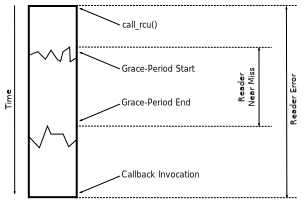
\includegraphics{debugging/RCUnearMiss}}
\caption{RCU Errors and Near Misses}
\label{fig:debugging:RCU Errors and Near Misses}
\end{figure}

예를 들어, 어떤 RCU 우선순위 부스팅의 낮은 확률 버그는 집중된 \co{rcutorture}
테스트에서 백시간마다 한번 가량 빌생했습니다.
이 버그의 확률이 상당히 줄었음을 99\,\% 확신하기 위해선 500 시간의 실패 없는
테스팅이 필요했으므로, 이 실패를 찾기 위한 \co{git bisect} 과정은 고통스럽게
느렸을 겁니다---또는 굉장히 커다란 테스트 환경이 필요했을 겁니다.
다행히도, 이 테스트 되는 RCU 오퍼레이션은 RCU grace period 대기만이 아니라
시작하기 위한 grace period 의 이전 대기, 그리고 이 RCU grace period 의 완료 후
RCU 콜백을 호출하기 위한 다음 대기를 포함했습니다.
\co{rcutorture} 에러와 거의 실수했음 사이의 이 차이가
Figure~\ref{fig:debugging:RCU Errors and Near Misses}
에 보여져 있습니다.
완벽한 오류의 요건을 갖추기 위해, 하나의 RCU read-side 크리티컬 섹션은 하나의
grace period 를 시작한 \co{call_rcu()} 로부터 앞의 grace period 의 남은 부분을
지나 \co{call_rcu()} 에 의해 시작된 grace period  전체를 지나 (구불거리는 선
사이의 영역으로 표시되었습니다), 이 grace period 의 종료로부터 콜백 호출 사이의
지연까지 지나도록 연장되어야 하는데, ``Error'' 화살표로 표시되어 있습니다.
그러나, RCU 의 정형적 정의는 RCU read-side 크리티컬 섹션이 단일 grace period 를
넘어 연장될 수 없게 하는데, ``Near Miss'' 화살표로 표시되어 있습니다.
이는 거의 실수함을 에러 조건으로 사용할 것을 추천하게 되지만, 언제 특정 grace
period 가 시작되고 끝났는지에 대해 구불거리는 선으로 표시된 것처럼 다른 CPU
들은 다른 의견을 가질 수 있으므로 문제가 됩니다.\footnote{
	실제 세계에서, idle CPU 는 많은 최근 grace period 를 완전히 인지하지
	못할 수 있으므로 이 선들은 훨씬 더 구불거릴 수 있습니다.}
따라서 이 거의 실수함을 오류로 사용하는 것은 false positive 를 초래할 수
있는데, 이는 자동화된 \co{rcutorture} 테스트에서는 지양되어야 합니다.

\iffalse

For example, a low-probability bug in RCU priority boosting occurred
roughly once every hundred hours of focused \co{rcutorture} testing.
Because it would take almost 500 hours of failure-free testing to be
99\,\% certain that the bug's probability had been significantly reduced,
the \co{git bisect} process
to find the failure would be painfully slow---or would require an extremely
large test farm.
Fortunately, the RCU operation being tested included not only a wait for
an RCU grace period, but also a previous wait for the grace period to start
and a subsequent wait for an RCU callback to be
invoked after completion of the RCU grace period.
This distinction between an \co{rcutorture} error and near miss is
shown in
Figure~\ref{fig:debugging:RCU Errors and Near Misses}.
To qualify as a full-fledged error, an RCU read-side critical section
must extend from the \co{call_rcu()} that initiated a grace period,
through the remainder of the previous grace period, through the
entirety of the grace period initiated by the \co{call_rcu()}
(denoted by the region between the jagged lines), and
through the delay from the end of that grace period to the callback
invocation, as indicated by the ``Error'' arrow.
However, the formal definition of RCU prohibits RCU read-side critical
sections from extending across a single grace period, as indicated by
the ``Near Miss'' arrow.
This suggests using near misses as the error condition, however, this
can be problematic because different CPUs can have different opinions
as to exactly where a given
grace period starts and ends, as indicated by the jagged lines.\footnote{
	In real life, these lines can be much more jagged because idle
	CPUs can be completely unaware of a great many recent grace
	periods.}
Using the near misses as the error condition could therefore result
in false positives, which need to be avoided in the automated
\co{rcutorture} testing.

\fi

운좋게도 \co{rcutorture} 는 grace period 의 거의 실수 버전에 민감한 일부 통계를
포함합니다.
앞서 이야기 했듯, 이 통계들은 RCU 의 상태 변수들로의 비동기적 액세스 덕에 false
positive 가 될 수 있지만, 이 false positive 는 IBM 메인프레임과 x86 같은 강한
순서 규칙 시스템에서는 굉장히 드물어서 천시간 테스팅 중 한번 정도 일어납니다.

이런 거의 실수함은 대략 한시간에 한번 일어나는데, 실제 실패보다 백배 이상 자주
일어나는 겁니다.
이런 거의 실수함을 사용하는 것은 이 버그의 근본 원인이 일주일도 안되어 파악될
수 있게 하였고 효과적이었음을 높은 수준으로 확신할 수 있는 수정사항을 하루도
안되어 만들 수 있게 했습니다.
대조적으로, 실제 오류만을 선호해 거의 실수함을 배제하는 것은 몇달의 디버깅과
검증 시간을 필요로 했을 겁니다.

거의 실수를 세는 것을 정리하자면, 일반적 접근법은 흔하지 않은 실패 세기를 그
실패와 연관되어 있을 것으로 여겨지며 더 흔한 거의 실수함으로 대체하는 것입니다.
이런 거의 실수함은 실제 실패의 heisenbug 에 대한 anti-heisenbug 로 여겨지는데,
거의 실수함은 더 흔하게 발생하고, 예를 들면 여러분이 디버깅을 위해 코드에
무언가를 추가하는 것 같은 코드 변경에 더 잘 버티기 때문입니다.

\iffalse

By sheer dumb luck, \co{rcutorture} happens to include some statistics that
are sensitive to the near-miss version of the grace period.
As noted above, these statistics are subject to false positives due to
their unsynchronized access to RCU's state variables,
but these false positives turn out to be extremely rare on strongly
ordered systems such as the IBM mainframe and x86, occurring less than
once per thousand hours of testing.

These near misses occurred roughly once per hour, about two orders of
magnitude more frequently than the actual errors.
Use of these near misses allowed the bug's root cause to be identified
in less than a week and a high degree of confidence in the fix to be
built in less than a day.
In contrast, excluding the near misses in favor of the real errors would
have required months of debug and validation time.

To sum up near-miss counting, the general approach is to replace counting
of infrequent failures with more-frequent near misses that are believed
to be correlated with those failures.
These near-misses can be considered an anti-heisenbug to the real failure's
heisenbug because the near-misses, being more frequent, are likely to
be more robust in the face of changes to your code, for example, the
changes you make to add debugging code.

\fi

\subsubsection{Heisenbug Discussion}
\label{sec:debugging:Heisenbug Discussion}

주의 깊은 독자는 이 섹션이
Section~\ref{sec:debugging:Statistics for Discrete Testing},
\ref{sec:debugging:Statistics Abuse for Discrete Testing},
그리고~\ref{sec:debuggingStatistics for Continuous Testing} 의 정교한 수학과
강력하게 대비될 만큼 흐릿하고 정성적이었음을 알아차렸을 수도 있을 겁니다.
여러분이 정교함과 수학을 사랑한다면, 이 섹션이 적용되는 상황이 앞의 섹션들이
적용되는 것들에 비해 훨씬 더 흔함에 실망할지도 모르겠습니다.

\iffalse

The alert reader might have noticed that this section was fuzzy and
qualitative, in stark contrast to the precise mathematics of
Sections~\ref{sec:debugging:Statistics for Discrete Testing},
\ref{sec:debugging:Statistics Abuse for Discrete Testing},
and~\ref{sec:debuggingStatistics for Continuous Testing}.
If you love precision and mathematics, you may be disappointed to
learn that the situations to which this section applies are far
more common than those to which the preceding sections apply.

\fi

사실, 더 흔한 경우는 여러분이 여러분의 코드에 버그가 있을 거라 믿는 이유가
있을지 몰라도 여러분은 어떤 그런 버그가 있는지, 무엇이 그것을 유발하는지, 그게
어떻게 발현되는지, 또는 어떤 조건이 그 발현의 확률에 영향을 주는지 모른다는
겁니다.
이 너무나도 흔한 경우에, 통계는 여러분을 돕지 못합니다.\footnote{
	여러분의 프로그램이 무엇을 할거라 기대되는지 여러분이 알고 있고
	여러분의 프로그램이 충분히 작다면 (여러분이 생각하는 경우는 아닐 확률이
	큽니다만),
	Chapter~\ref{chp:Formal Verification} 에서 설명되는
	정형적 검증 도구가 도움될 겁니다.}
즉, 통계는 여러분을 \emph{직접적으로} 돕지 못합니다.
그러나 통계는 \emph{만약} 여러분이 실수할 수 있음을 인정하는데 필요한 겸손을
가지고 있다면, 그 실수의 확률을 줄일 수 있다면 (예를 들어, 충분히 잠을 자는
식으로), 여러분이 과거에 만든 실수의 종류와 수가 미래에 만들 실수의 종류와 수를
말해준다면 큰 도움이 될 수 있습니다.
예를 들어, 저는 초기화 코드의 작지만 중요한, 그리고 대부분의 또는 심지어 전체
병렬 프로그램을 정확하게 하는 작지만 중요한 부분을 잊는 안타까운 경향을
갖습니다---초기화에서의 멍청한 누락을 제외하고요.
일단 제가 저는 이런 종류의 실수에 취약함을 인정하면, 저 스스로를 제 초기화
코드를 재차 확인하게끔 하는게 조금 더 쉬워졌습니다 (하지만 쉽지 않았습니다!).
이렇게 하는건 제가 시간 내에 많은 버그를 찾을 수 있게 해줬습니다.

\iffalse

In fact, the common case is that although you might have reason to believe
that your code has bugs, you have no idea what those bugs are, what
causes them, how likely they are to appear, or what conditions affect
their probability of appearance.
In this all-too-common case, statistics cannot help you.\footnote{
	Although if you know what your program is supposed to do and
	if your program is small enough (both less likely that you
	might think), then the formal-verification tools described in
	Chapter~\ref{chp:Formal Verification}
	can be helpful.}
That is to say, statistics cannot help you \emph{directly}.
But statistics can be of great indirect help---\emph{if} you have the
humility required to admit that you make mistakes, that you can reduce the
probability of these mistakes (for example, by getting enough sleep), and
that the number and type of mistakes you made in the past is indicative of
the number and type of mistakes that you are likely to make in the future.
For example, I have a deplorable tendency to forget to write a small
but critical portion of the initialization code, and frequently get most
or even all of a parallel program correct---except for a stupid
omission in initialization.
Once I was willing to admit to myself that I am prone to this type of
mistake, it was easier (but not easy!) to force myself to double-check
my initialization code.
Doing this allowed me to find numerous bugs ahead of time.

\fi

Taleb 의 명명법~\cite{NassimTaleb2007BlackSwan} 을 사용하자면, 백조는 우리가
재현할 수 있는 버그입니다.
우린 많은 수의 테스트를 수행하고 버그의 확률을 추정하는데 일반적인 통계를
사용하고, 제안된 수정사항에 대한 우리의 자신감을 추정하는데에 일반적 통계를 또
사용할 수 있습니다.
기대되지 않은 버그는 흑조입니다.
우린 그것에 대해 무엇도 모르고, 그게 일어나게 한 어떤 테스트도 없으며, 통계는
도움이 되지 않습니다.
우리의 행동, 특히 우리가 만드는 실수들의 수와 종류를 연구하는 것은, 흑조를
회색조로 만들 수 있습니다.
우린 그 버그가 정확히 무엇인지는 모를 수도 있지만 그것의 수와 어쩌면 그 종류에
대한 어떤 아이디어를 얻을 수도 있습니다.
일반적인 통계는 여전히 도움이 되지 않지만 (우리가 그 버그들 중 하나를 재현할 수
있기 전까지는요) 튼튼한 테스트 방법은\footnote{
	brutal 이라고도 이야기 되지요.}
큰 도움이 될 수 있습니다.
따라서 목표는 흑조를 회색으로 바꾸기 위해 경험과 좋은 검증 수법들을 사용하고,
집중된 테스트와 분석을 통해 회색조를 흰색으로 바꾸고, 이 백조를 고치기 위해
일반적 방법을 사용하는 것입니다.

\iffalse

Using Taleb's nomenclature~\cite{NassimTaleb2007BlackSwan},
a white swan is a bug that we can reproduce.
We can run a large number of tests, use ordinary statistics to
estimate the bug's probability, and use ordinary statistics again
to estimate our confidence in a proposed fix.
An unsuspected bug is a black swan.
We know nothing about it, we have no tests that have yet caused it
to happen, and statistics is of no help.
Studying our own behavior, especially the number and types of mistakes
we make, can turn black swans into grey swans.
We might not know exactly what the bugs are, but we have some idea of
their number and maybe also of their type.
Ordinary statistics is still of no help (at least not until we are
able to reproduce one of the bugs), but robust\footnote{
	That is to say brutal.}
testing methods can be of great help.
The goal, therefore, is to use experience and good validation practices
to turn the black swans grey, focused testing and analysis to turn the
grey swans white, and ordinary methods to fix the white swans.

\fi

그러나, 지금까지 우리는 병렬 프로그램의 기능에서의 버그에만 집중했습니다.
하지만, 성능이 병렬 프로그램에서의 첫번째 요구사항이므로 (아니라면, 왜 순차적
프로그램을 작성하지 않습니까?), 다음 섹션은 성능 버그에 대해 이야기 해봅니다.

\iffalse

That said, thus far, we have focused solely on bugs in the parallel program's
functionality.
However, because performance is a first-class requirement for a
parallel program (otherwise, why not write a sequential program?),
the next section discusses performance bugs.

\fi

\section{Performance Estimation}
\label{sec:debugging:Performance Estimation}
%
\epigraph{There are lies, damn lies, statistics, and benchmarks.}
	 {\emph{Unknown}}

Parallel programs usually have performance and scalability requirements,
after all, if performance is not an issue, why not use a sequential
program?
Ultimate performance and linear scalability might not be necessary, but
there is little use for a parallel program that runs slower than its
optimal sequential counterpart.
And there really are cases where every microsecond matters and every
nanosecond is needed.
Therefore, for parallel programs, insufficient performance is just as
much a bug as is incorrectness.

\QuickQuizSeries{%
\QuickQuizB{
	That is ridiculous!!!
	After all, isn't getting the correct answer later than one would like
	better than getting an incorrect answer???
}\QuickQuizAnswerB{
	This question fails to consider the option of choosing not to
	compute the answer at all, and in doing so, also fails to consider
	the costs of computing the answer.
	For example, consider short-term weather forecasting, for which
	accurate models exist, but which require large (and expensive)
	clustered supercomputers, at least if you want to actually run
	the model faster than the weather.

	And in this case, any performance bug that prevents the model from
	running faster than the actual weather prevents any forecasting.
	Given that the whole purpose of purchasing the large clustered
	supercomputers was to forecast weather, if you cannot run the
	model faster than the weather, you would be better off not running
	the model at all.

	More severe examples may be found in the area of safety-critical
	real-time computing.
}\QuickQuizEndB
%
\QuickQuizE{
	But if you are going to put in all the hard work of parallelizing
	an application, why not do it right?
	Why settle for anything less than optimal performance and
	linear scalability?
}\QuickQuizAnswerE{
	Although I do heartily salute your spirit and aspirations,
	you are forgetting that there may be high costs due to delays
	in the program's completion.
	For an extreme example, suppose that a 40\,\% performance shortfall
	from a single-threaded application is causing one person to die
	each day.
	Suppose further that in a day you could hack together a
	quick and dirty
	parallel program that ran 50\,\% faster on an eight-CPU system
	than the sequential version, but that an optimal parallel
	program would require four months of painstaking design, coding,
	debugging, and tuning.

	It is safe to say that more than 100 people would prefer the
	quick and dirty version.
}\QuickQuizEndE
}

Validating a parallel program must therfore include validating its
performance.
But validating performance means having a workload to run and performance
criteria with which to evaluate the program at hand.
These needs are often met by \emph{performance benchmarks}, which
are discussed in the next section.

\subsection{Benchmarking}
\label{sec:debugging:Benchmarking}

Frequent abuse aside, benchmarks are both useful and heavily used,
so it is not helpful to be too dismissive of them.
Benchmarks span the range from ad hoc test jigs to international
standards, but regardless of their level of formality, benchmarks
serve four major purposes:

\begin{enumerate}
\item	Providing a fair framework for comparing competing implementations.
\item	Focusing competitive energy on improving implementations in ways
	that matter to users.
\item	Serving as example uses of the implementations being benchmarked.
\item	Serving as a marketing tool to highlight your software
	against your competitors' offerings.
\end{enumerate}

Of course,  the only completely fair framework is the intended
application itself.
So why would anyone who cared about fairness in benchmarking
bother creating imperfect benchmarks rather than simply
using the application itself as the benchmark?

Running the actual application is in fact the best approach where it is practical.
Unfortunately, it is often impractical for the following reasons:

\begin{enumerate}
\item	The application might be proprietary, and you
	might not have the right to run the intended application.
\item	The application might require more hardware
	than you have access to.
\item	The application might use data that you cannot
	access, for example, due to privacy regulations.
\item	The application might take longer than is convenient to
	reproduce a performance or scalability problem.\footnote{
		Microbenchmarks can help, but
		please see \cref{sec:debugging:Microbenchmarking}.}
\end{enumerate}

Creating a benchmark that approximates
the application can help overcome these obstacles.
A carefully constructed benchmark can help promote performance,
scalability, energy efficiency, and much else besides.
However, be careful to avoid investing too much into the benchmarking
effort.
It is after all important to invest at least a little into the
application itself~\cite{Gray91}.

\subsection{Profiling}
\label{sec:debugging:Profiling}

In many cases, a fairly small portion of your software is responsible
for the majority of the performance and scalability shortfall.
However, developers are notoriously unable to identify the actual
bottlenecks by inspection.
For example, in the case of a kernel buffer allocator, all attention focused
on a search of a dense array which turned out to represent only
a few percent of the allocator's execution time.
An execution profile collected via a logic analyzer focused attention
on the cache misses that were actually responsible for the majority
of the problem~\cite{McKenney93}.

An old-school but quite effective method of tracking down performance
and scalability bugs is to run your program under a debugger,
then periodically interrupt it, recording the stacks of all threads
at each interruption.
The theory here is that if something is slowing down your program,
it has to be visible in your threads' executions.

That said, there are a number of tools
that will usually do a much better job of helping you to focus your
attention where it will do the most good.
Two popular choices are \co{gprof} and \co{perf}.
To use \co{perf} on a single-process program, prefix your command
with \co{perf record}, then after the command completes, type
\co{perf report}.
There is a lot of work on tools for performance debugging of multi-threaded
programs, which should make this important job easier.
Again, one good starting point is Brendan Gregg's blog.\footnote{
	\url{http://www.brendangregg.com/blog/}}

\subsection{Differential Profiling}
\label{sec:debugging:Differential Profiling}

Scalability problems will not necessarily be apparent unless you are running
on very large systems.
However, it is sometimes possible to detect impending scalability problems
even when running on much smaller systems.
One technique for doing this is called \emph{differential profiling}.

The idea is to run your workload under two different sets of conditions.
For example, you might run it on two CPUs, then run it again on four
CPUs.
You might instead vary the load placed on the system, the number of
network adapters, the number of mass-storage devices, and so on.
You then collect profiles of the two runs, and mathematically combine
corresponding profile measurements.
For example, if your main concern is scalability, you might take the
ratio of corresponding measurements, and then sort the ratios into
descending numerical order.
The prime scalability suspects will then be sorted to the top of the
list~\cite{McKenney95a,McKenney99b}.

Some tools such as \co{perf} have built-in differential-profiling
support.

\subsection{Microbenchmarking}
\label{sec:debugging:Microbenchmarking}

Microbenchmarking can be useful when deciding which algorithms or
data structures are worth incorporating into a larger body of software
for deeper evaluation.

One common approach to microbenchmarking is to measure the time,
run some number of iterations of the code
under test, then measure the time again.
The difference between the two times divided by the number of iterations
gives the measured time required to execute the code under test.

Unfortunately, this approach to measurement allows any number of errors
to creep in, including:

\begin{enumerate}
\item	The measurement will include some of the overhead of
	the time measurement.
	This source of error can be reduced to an arbitrarily small
	value by increasing the number of iterations.
\item	The first few iterations of the test might incur cache misses
	or (worse yet) page faults that might inflate the measured
	value.
	This source of error can also be reduced by increasing the
	number of iterations, or it can often be eliminated entirely
	by running a few warm-up iterations before starting the
	measurement period.
	Most systems have ways of detecting whether a given process
	incurred a page fault, and you should make use of this to
	reject runs whose performance has been thus impeded.
\item	Some types of interference, for example, random memory errors,
	are so rare that they can be dealt with by running a number
	of sets of iterations of the test.
	If the level of interference was statistically significant,
	any performance outliers could be rejected statistically.
\item	Any iteration of the test might be interfered with by other
	activity on the system.
	Sources of interference include other applications, system
	utilities and daemons, device interrupts, firmware interrupts
	(including system management interrupts, or SMIs),
	virtualization, memory errors, and much else besides.
	Assuming that these sources of interference occur randomly,
	their effect can be minimized by reducing the number of
	iterations.
\item	Thermal throttling can understate scalability because increasing
	CPU activity increases heat generation, and on systems without
	adequate cooling (most of them!), this can result in the CPU
	frequency decreasing as the number of CPUs increases.\footnote{
		Systems with adequate cooling tend to look like gaming systems.}
	Of course, if you are testing an application to evaluate its
	expected behavior when run in production, such thermal throttling
	is simply a fact of life.
	Otherwise, if you are interested in theoretical scalability,
	use a system with adequate cooling or reduce the CPU clock rate
	to a level that the cooling system can handle.
\end{enumerate}

The first and fourth sources of interference provide conflicting advice,
which is one sign that we are living in the real world.
The remainder of this section looks at ways of resolving this conflict.

\QuickQuiz{
	But what about other sources of error, for example, due to
	interactions between caches and memory layout?
}\QuickQuizAnswer{
	Changes in memory layout can indeed result in unrealistic
	decreases in execution time.
	For example, suppose that a given microbenchmark almost
	always overflows the L0 cache's associativity, but with just the right
	memory layout, it all fits.
	If this is a real concern, consider running your microbenchmark
	using huge pages (or within the kernel or on bare metal) in
	order to completely control the memory layout.

	But note that there are many different possible memory-layout
	bottlenecks.
	Benchmarks sensitive to memory bandwidth (such as those involving
	matrix arithmetic) should spread the running threads across the
	available cores and sockets to maximize memory parallelism.
	They should also spread the data across NUMA nodes, memory
	controllers, and DRAM chips to the extent possible.
	In contrast, benchmarks sensitive to memory latency (including
	most poorly scaling applications) should instead maximize
	locality, filling each core and socket in turn before adding
	another one.
}\QuickQuizEnd

The following sections discuss ways of dealing with these measurement
errors, with
Section~\ref{sec:debugging:Isolation}
covering isolation techniques that may be used to prevent some forms of
interference,
and with
Section~\ref{sec:debugging:Detecting Interference}
covering methods for detecting interference so as to reject measurement
data that might have been corrupted by that interference.

\subsection{Isolation}
\label{sec:debugging:Isolation}

The Linux kernel provides a number of ways to isolate a group of
CPUs from outside interference.

First, let's look at interference by other processes, threads, and tasks.
The POSIX \co{sched_setaffinity()} system call may be used to move
most tasks off of a given set of CPUs and to confine your tests to
that same group.
The Linux-specific user-level \co{taskset} command may be used for
the same purpose, though both \co{sched_setaffinity()} and
\co{taskset} require elevated permissions.
Linux-specific control groups (cgroups) may be used for this same purpose.
This approach can be quite effective at reducing interference, and
is sufficient in many cases.
However, it does have limitations, for example, it cannot do anything
about the per-CPU kernel threads that are often used for housekeeping
tasks.

One way to avoid interference from per-CPU kernel threads is to run
your test at a high real-time priority, for example, by using
the POSIX \co{sched_setscheduler()} system call.
However, note that if you do this, you are implicitly taking on
responsibility for avoiding infinite loops, because otherwise
your test can prevent part of the kernel from functioning.
This is an example of the Spiderman Principle: ``With great
power comes great responsibility.''
And although the default real-time throttling settings often address
such problems, they might do so by causing your real-time threads
to miss their deadlines.

These approaches can greatly reduce, and perhaps even eliminate,
interference from processes, threads, and tasks.
However, it does nothing to prevent interference from device
interrupts, at least in the absence of threaded interrupts.
Linux allows some control of threaded interrupts via the
\path{/proc/irq} directory, which contains numerical directories, one
per interrupt vector.
Each numerical directory contains \co{smp_affinity} and
\co{smp_affinity_list}.
Given sufficient permissions, you can write a value to these files
to restrict interrupts to the specified set of CPUs.
For example, either
``\co{echo 3 > /proc/irq/23/smp_affinity}''
or
``\co{echo 0-1 > /proc/irq/23/smp_affinity_list}''
would confine interrupts on vector~23 to CPUs~0 and~1,
at least given sufficient privileges.
You can use ``\co{cat /proc/interrupts}'' to obtain a list of the interrupt
vectors on your system, how many are handled by each CPU, and what
devices use each interrupt vector.

Running a similar command for all interrupt vectors on your system
would confine interrupts to CPUs~0 and~1, leaving the remaining CPUs
free of interference.
Or mostly free of interference, anyway.
It turns out that the scheduling-clock interrupt fires on each CPU
that is running in user mode.\footnote{
	Frederic Weisbecker leads up a \co{NO_HZ_FULL}
	adaptive-ticks project
	that allows scheduling-clock interrupts to be disabled
	on CPUs that have only one runnable task.
	As of 2021, this is largely complete.}
In addition you must take care to ensure that the set of CPUs that you
confine the interrupts to is capable of handling the load.

But this only handles processes and interrupts running in the same
operating-system instance as the test.
Suppose that you are running the test in a guest OS that is itself
running on a hypervisor, for example, Linux running KVM?
Although you can in theory apply the same techniques at the hypervisor
level that you can at the guest-OS level, it is quite common for
hypervisor-level operations to be restricted to authorized personnel.
In addition, none of these techniques work against firmware-level
interference.

\QuickQuiz{
	Wouldn't the techniques suggested to isolate the code under
	test also affect that code's performance, particularly if
	it is running within a larger application?
}\QuickQuizAnswer{
	Indeed it might, although in most microbenchmarking efforts
	you would extract the code under test from the enclosing
	application.
	Nevertheless, if for some reason you must keep the code under
	test within the application, you will very likely need to use
	the techniques discussed in
	Section~\ref{sec:debugging:Detecting Interference}.
}\QuickQuizEnd

Of course, if it is in fact the interference that is producing the
behavior of interest, you will instead need to promote interference,
in which case being unable to prevent it is not a problem.
But if you really do need interference-free measurements, then instead
of preventing the interference, you might need to detect the interference
as described in the next section.

\subsection{Detecting Interference}
\label{sec:debugging:Detecting Interference}

If you cannot prevent interference, perhaps you can detect it
and reject results from any affected test runs.
Section~\ref{sec:debugging:Detecting Interference Via Measurement}
describes methods of rejection involving additional measurements,
while Section~\ref{sec:debugging:Detecting Interference Via Statistics}
describes statistics-based rejection.

\subsubsection{Detecting Interference Via Measurement}
\label{sec:debugging:Detecting Interference Via Measurement}

%	Sources of interference include other applications, system
%	utilities and daemons, device interrupts, firmware interrupts
%	(including system management interrupts, or SMIs),
%	virtualization, memory errors, and much else besides.

Many systems, including Linux, provide means for determining after the
fact whether some forms of interference have occurred.
For example, process-based interference results in context switches,
which, on Linux-based systems, are visible in
\path{/proc/<PID>/sched} via the \co{nr_switches} field.
Similarly, interrupt-based interference can be detected via the
\path{/proc/interrupts} file.

\begin{listing}[tb]
\begin{fcvlabel}[ln:debugging:Using getrusage() to Detect Context Switches]
\begin{VerbatimL}
#include <sys/time.h>
#include <sys/resource.h>

/* Return 0 if test results should be rejected. */
int runtest(void)
{
	struct rusage ru1;
	struct rusage ru2;

	if (getrusage(RUSAGE_SELF, &ru1) != 0) {
		perror("getrusage");
		abort();
	}
	/* run test here. */
	if (getrusage(RUSAGE_SELF, &ru2 != 0) {
		perror("getrusage");
		abort();
	}
	return (ru1.ru_nvcsw == ru2.ru_nvcsw &&
	        ru1.runivcsw == ru2.runivcsw);
}
\end{VerbatimL}
\end{fcvlabel}
\caption{Using \tco{getrusage()} to Detect Context Switches}
\label{lst:debugging:Using getrusage() to Detect Context Switches}
\end{listing}

Opening and reading files is not the way to low overhead, and it is
possible to get the count of context switches for a given thread
by using the \co{getrusage()} system call, as shown in
Listing~\ref{lst:debugging:Using getrusage() to Detect Context Switches}.
This same system call can be used to detect minor page faults (\co{ru_minflt})
and major page faults (\co{ru_majflt}).

Unfortunately, detecting memory errors and firmware interference is quite
system-specific, as is the detection of interference due to virtualization.
Although avoidance is better than detection, and detection is better than
statistics, there are times when one must avail oneself of statistics,
a topic addressed in the next section.

\subsubsection{Detecting Interference Via Statistics}
\label{sec:debugging:Detecting Interference Via Statistics}

Any statistical analysis will be based on assumptions about the data,
and performance microbenchmarks often support the following assumptions:

\begin{enumerate}
\item	Smaller measurements are more likely to be accurate than
	larger measurements.
\item	The measurement uncertainty of good data is known.
\item	A reasonable fraction of the test runs will result in good data.
\end{enumerate}

The fact that smaller measurements are more likely to be accurate than
larger measurements suggests that sorting the measurements in increasing
order is likely to be productive.\footnote{
	To paraphrase the old saying, ``Sort first and ask questions later.''}
The fact that the measurement uncertainty is known allows us to accept
measurements within this uncertainty of each other:  If the effects of
interference are large compared to this uncertainty, this will ease
rejection of bad data.
Finally, the fact that some fraction (for example, one third) can be
assumed to be good allows us to blindly accept the first portion of the
sorted list, and this data can then be used to gain an estimate of the
natural variation of the measured data, over and above the assumed
measurement error.

The approach is to take the specified number of leading elements from the
beginning of the sorted list, and use these to estimate a typical
inter-element delta, which in turn may be multiplied by the number of
elements in the list to obtain an upper bound on permissible values.
The algorithm then repeatedly considers the next element of the list.
If it falls below the upper bound, and if the distance between
the next element and the previous element is not too much greater than
the average inter-element distance for the portion of the list accepted
thus far, then the next element is accepted and the process repeats.
Otherwise, the remainder of the list is rejected.

\begin{listing}[tb]
\input{CodeSamples/debugging/datablows@whole.fcv}
\caption{Statistical Elimination of Interference}
\label{lst:debugging:Statistical Elimination of Interference}
\end{listing}

Listing~\ref{lst:debugging:Statistical Elimination of Interference}
shows a simple \co{sh}/\co{awk} script implementing this notion.
Input consists of an x-value followed by an arbitrarily long list of y-values,
and output consists of one line for each input line, with fields as follows:

\begin{enumerate}
\item	The x-value.
\item	The average of the selected data.
\item	The minimum of the selected data.
\item	The maximum of the selected data.
\item	The number of selected data items.
\item	The number of input data items.
\end{enumerate}

This script takes three optional arguments as follows:

\begin{description}
\item	[\lopt{divisor}\nf{:}] Number of segments to divide the list
	into, for example, a divisor of four means that the first quarter of
	the data elements will be assumed to be good.
	This defaults to three.
\item	[\lopt{relerr}\nf{:}] Relative measurement error.  The script
	assumes that values that differ by less than this error are for all
	intents and purposes equal.
	This defaults to 0.01, which is equivalent to 1\,\%.
\item	[\lopt{trendbreak}\nf{:}] Ratio of inter-element spacing
	constituting a break in the trend of the data.
	For example, if the average spacing in the data accepted so far
	is 1.5, then if the trend-break ratio is 2.0, then if the next
	data value differs from the last one by more than 3.0, this
	constitutes a break in the trend.
	(Unless of course, the relative error is greater than 3.0, in
	which case the ``break'' will be ignored.)
\end{description}

\begin{fcvref}[ln:debugging:datablows:whole]
\Clnrefrange{param:b}{param:e} of
Listing~\ref{lst:debugging:Statistical Elimination of Interference}
set the default values for the parameters, and
\clnrefrange{parse:b}{parse:e} parse
any command-line overriding of these parameters.
\end{fcvref}
\begin{fcvref}[ln:debugging:datablows:whole:awk]
The \co{awk} invocation on line~\lnref{invoke} sets the values of the
\co{divisor}, \co{relerr}, and \co{trendbreak} variables to their
\co{sh} counterparts.
In the usual \co{awk} manner,
\clnrefrange{copy:b}{end} are executed on each input
line.
The loop spanning lines~\lnref{copy:b} and~\lnref{copy:e} copies
the input y-values to the
\co{d} array, which line~\lnref{asort} sorts into increasing order.
Line~\lnref{comp_i} computes the number of trustworthy y-values
by applying \co{divisor} and rounding up.

\Clnrefrange{delta}{comp_max:e} compute the \co{maxdelta}
lower bound on the upper bound of y-values.
To this end, line~\lnref{maxdelta} multiplies the difference in values over
the trusted region of data by the \co{divisor}, which projects the
difference in values across the trusted region across the entire
set of y-values.
However, this value might well be much smaller than the relative error,
so line~\lnref{maxdelta1} computes the absolute error (\co{d[i] * relerr})
and adds
that to the difference \co{delta} across the trusted portion of the data.
Lines~\lnref{comp_max:b} and~\lnref{comp_max:e} then compute the maximum of
these two values.

Each pass through the loop spanning \clnrefrange{add:b}{add:e}
attempts to add another
data value to the set of good data.
\Clnrefrange{chk_engh}{break} compute the trend-break delta,
with line~\lnref{chk_engh} disabling this
limit if we don't yet have enough values to compute a trend,
and with line~\lnref{mul_avr} multiplying \co{trendbreak} by the average
difference between pairs of data values in the good set.
If line~\lnref{chk_max} determines that the candidate data value would exceed the
lower bound on the upper bound (\co{maxdelta}) \emph{and}
that the difference between the candidate data value
and its predecessor exceeds the trend-break difference (\co{maxdiff}),
then line~\lnref{break} exits the loop: We have the full good set of data.

\Clnrefrange{comp_stat:b}{comp_stat:e} then compute and print
statistics.
\end{fcvref}

\QuickQuizSeries{%
\QuickQuizB{
	This approach is just plain weird!
	Why not use means and standard deviations, like we were taught
	in our statistics classes?
}\QuickQuizAnswerB{
	Because mean and standard deviation were not designed to do this job.
	To see this, try applying mean and standard deviation to the
	following data set, given a 1\,\% relative error in measurement:

	\begin{quote}
		49,548.4 49,549.4 49,550.2 49,550.9 49,550.9 49,551.0
		49,551.5 49,552.1 49,899.0 49,899.3 49,899.7 49,899.8
		49,900.1 49,900.4 52,244.9 53,333.3 53,333.3 53,706.3
		53,706.3 54,084.5
	\end{quote}

	The problem is that mean and standard deviation do not rest on
	any sort of measurement-error assumption, and they will therefore
	see the difference between the values near 49,500 and those near
	49,900 as being statistically significant, when in fact they are
	well within the bounds of estimated measurement error.

	Of course, it is possible to create a script similar to
	that in
	Listing~\ref{lst:debugging:Statistical Elimination of Interference}
	that uses standard deviation rather than absolute difference
	to get a similar effect,
	and this is left as an exercise for the interested reader.
	Be careful to avoid divide-by-zero errors arising from strings
	of identical data values!
}\QuickQuizEndB
%
\QuickQuizE{
	But what if all the y-values in the trusted group of data
	are exactly zero?
	Won't that cause the script to reject any non-zero value?
}\QuickQuizAnswerE{
	Indeed it will!
	But if your performance measurements often produce a value of
	exactly zero, perhaps you need to take a closer look at your
	performance-measurement code.

	Note that many approaches based on mean and standard deviation
	will have similar problems with this sort of dataset.
}\QuickQuizEndE
}

Although statistical interference detection can be quite useful, it should
be used only as a last resort.
It is far better to avoid interference in the first place
(Section~\ref{sec:debugging:Isolation}), or, failing that,
detecting interference via measurement
(Section~\ref{sec:debugging:Detecting Interference Via Measurement}).

\section{Summary}
\label{sec:debugging:Summary}
%
% \epigraph{To err is human---but it feels devine.}{\emph{Mae West}}
\epigraph{To err is human!  Stop being human!!!}{\emph{Ed Nofziger}}

\begin{figure}[tbp]
\centering
\resizebox{3in}{!}{\includegraphics{cartoons/UseTheRightCannon}}
\caption{Choose Validation Methods Wisely}
\ContributedBy{Figure}{fig:debugging:Choose Validation Methods Wisely}{Melissa Broussard}
\end{figure}

Although validation never will be an exact science, much can be gained
by taking an organized approach to it, as an organized approach will
help you choose the right validation tools for your job, avoiding
situations like the one fancifully depicted in
Figure~\ref{fig:debugging:Choose Validation Methods Wisely}.

A key choice is that of statistics.
Although the methods described in this chapter work very well most of
the time, they do have their limitations, courtesy of the Halting
Problem~\cite{AlanMTuring1937HaltingProblem,GeoffreyKPullum2000HaltingProblem}.
Fortunately for us, there is a huge number of special cases in which
we can not only work out whether a program will halt, but also
estimate how long it will run before halting, as discussed in
Section~\ref{sec:debugging:Performance Estimation}.
Furthermore, in cases where a given program might or might not work
correctly, we can often establish estimates for what fraction of the
time it will work correctly, as discussed in
Section~\ref{sec:debugging:Probability and Heisenbugs}.

Nevertheless, unthinking reliance on these estimates is brave to the
point of foolhardiness.
After all, we are summarizing a huge mass of complexity in code and
data structures down to a single solitary number.
Even though we can get away with such bravery a surprisingly large
fraction of the time, abstracting all that code and data away will
occasionally cause severe problems.

One possible problem is variability, where repeated runs give wildly
different results.
This problem is often addressed using standard deviation, however, using
two numbers to summarize the behavior of a large and complex program is
about as brave as using only one number.
In computer programming, the surprising thing is that use of the
mean or the mean and standard deviation are often sufficient.
Nevertheless, there are no guarantees.

One cause of variation is confounding factors.
For example, the CPU time consumed by a linked-list search will depend
on the length of the list.
Averaging together runs with wildly different list lengths will
probably not be useful, and adding a standard deviation to the mean
will not be much better.
The right thing to do would be control for list length, either by
holding the length constant or to measure CPU time as a function of
list length.

Of course, this advice assumes that you are aware of the confounding
factors, and Murphy says that you will not be.
I have been involved in projects that had confounding factors as diverse
as air conditioners (which drew considerable power at startup, thus
causing the voltage supplied to the computer to momentarily drop too
low, sometimes resulting in failure), cache state (resulting in odd
variations in performance), I/O errors (including disk errors, packet
loss, and duplicate Ethernet MAC addresses), and even porpoises (which
could not resist playing with an array of transponders, which could be
otherwise used for high-precision acoustic positioning and navigation).
And this is but one reason why a good night's sleep is such an effective
debugging tool.

In short, validation always will require some measure of the behavior of
the system.
To be at all useful, this measure must be a severe summarization of the
system, which in turn means that it can be misleading.
So as the saying goes, ``Be careful.  It is a real world out there.''

But what if you are working on the Linux kernel, which as of 2017 was
estimated to have more than 20 billion instances running throughout
the world?
In that case, a bug that occurs once every million years on a single system
will be encountered more than 50 times per day across the installed base.
A test with a 50\,\% chance of encountering this bug in a one-hour run
would need to increase that bug's probability of occurrence by more than
ten orders of magnitude, which poses a severe challenge to
today's testing methodologies.
One important tool that can sometimes be applied with good effect to
such situations is formal verification, the subject of the next chapter,
and, more speculatively, Section~\ref{sec:future:Formal Regression Testing?}.

The topic of choosing a validation plan, be it testing, formal
verification, or both, is taken up by
\cref{sec:formal:Choosing a Validation Plan}.

\QuickQuizAnswersChp{qqzdebugging}

% @@@ Test on varying CPU speeds.  Or on multi-socket systems.
